%----------------------------------------------------------------------------------------
% Preambulo y Configuración
%----------------------------------------------------------------------------------------

\documentclass[
    11pt,
    spanish,
    singlespacing,
    parskip,
    headsepline,
    bookmarks=true,
    unicode=true,
    pdftoolbar=true,
    pdfmenubar=true,
    pdffitwindow=false,
    colorlinks=true,
    linkcolor=blue,
    citecolor=blue,
    urlcolor=blue
]{MastersDoctoralThesis}

\usepackage[utf8]{inputenc} % Codificación de entrada UTF-8
\usepackage[T1]{fontenc}    % Codificación de salida para caracteres especiales
\usepackage{graphicx}       % Manejo de gráficos
\usepackage{eso-pic}        % Permite agregar fondos
\usepackage{hyperref}       % Manejo de hipervínculos y marcadores
\usepackage{float} 
\usepackage{comment}
\usepackage{listings}
\usepackage{seqsplit}
\usepackage[htt]{hyphenat}
\usepackage{caption}
\usepackage{booktabs}
\usepackage{multirow}
\usepackage{siunitx}
\usepackage{xcolor}


% Redefinición de caracteres problemáticos en marcadores
\hypersetup{
    pdftitle={Título del Documento},
    pdfauthor={Autor del Documento},
    pdfkeywords={Sistemas Embebidos, Internet de las Cosas, Inteligencia Artificial},
    pdfstartview={FitH},
    unicode=true,
    colorlinks=true,
    linkcolor=blue,
    citecolor=blue,
    urlcolor=blue
}

\pdfstringdefDisableCommands{%
  \def\texttt#1{#1}%
  \def\textbf#1{#1}%
  \def\textit#1{#1}%
  \def\"{\"}%
  \def\~{~}%
  \def\'{'}%
  \def\^{}%
  \def\textunderscore{\_} % Manejo del subrayado en marcadores
}

% Definición de estilo para código Swift (si no está definido globalmente)
\lstdefinelanguage{Swift}{
  keywords={class, func, var, let, if, else, guard, return, enum, case,
            struct, protocol, import, switch, self, true, false, nil, try,
            catch, throw, throws, weak, private, public, internal, static,
            override, init, deinit, extension, where, associatedtype,
            typealias, some, await, async, @Published, @StateObject,
            @State, @main, @ObservedObject},
  sensitive=true,
  comment=[l]{//},
  morecomment=[s]{/*}{*/},
  string=[b]",
  morestring=[b]',
}

\lstset{
  language=Swift,
  basicstyle=\ttfamily\small,
  keywordstyle=\bfseries\color{blue!70!black},
  commentstyle=\itshape\color{gray},
  stringstyle=\color{red!70!black},
  breaklines=true,
  frame=single,
  numbers=left,
  numberstyle=\tiny\color{gray},
  tabsize=4,
  showstringspaces=false,
  captionpos=b,
}


% Ajusta el valor de 'skip' a los puntos (pt), milímetros (mm) o centímetros (cm) que prefieras.
\captionsetup{skip=15pt}
\setlength{\abovecaptionskip}{15pt} % Controla el espacio ENTRE la imagen y el caption
\setlength{\belowcaptionskip}{5pt}  % Controla el espacio DEBAJO del caption

% Definir comandos requeridos por la clase
\newcommand{\degreename}{Maestría en Ciencias} % Cambia según tu título
\newcommand{\univname}{Universidad Nacional de Ejemplo} % Cambia según tu universidad
\newcommand{\keywordnames}{Palabras clave:}
%----------------------------------------------------------------------------------------
% Documento Principal
%----------------------------------------------------------------------------------------

\begin{document}

% Configuración de la portada
\posgrado{Carrera / Maestría}
\keywords{Sistemas Embebidos, Internet de las Cosas, Inteligencia Artificial}

% Incluir la portada desde un archivo separado
\include{portada}

% Configuración del contenido preliminar
\frontmatter % Usar numeración romana para las páginas preliminares
\pagestyle{plain} % Estilo de encabezado simple

%----------------------------------------------------------------------------------------
% Resumen
%----------------------------------------------------------------------------------------

\begin{abstract}
\addchaptertocentry{\abstractname} % Agregar resumen al índice
En la presente memoria se desarrolla una prueba de concepto de una aplicación móvil nativa para iOS, capaz de procesar comandos de voz e interpretar intenciones transaccionales de forma 100\% local. Este sistema fue desarrollado para ser validado por el equipo de Identidad Digital del Banco Galicia Minorista.

Para su materialización, se utilizaron herramientas del ecosistema Apple como Swift, Xcode, la API AVFoundation y el framework Core ML.


\end{abstract}

%----------------------------------------------------------------------------------------
% Índice
%----------------------------------------------------------------------------------------

\tableofcontents
\listoffigures
\listoftables

%----------------------------------------------------------------------------------------
% Capítulos
%----------------------------------------------------------------------------------------

\mainmatter % Iniciar numeración numérica para el contenido principal
\pagestyle{thesis} % Estilo de encabezado de tesis

% Incluir capítulos desde archivos separados
% Chapter 1

\chapter{Introducción general} % Main chapter title

\label{Chapter1} % For referencing the chapter elsewhere, use \ref{Chapter1} 
\label{IntroGeneral}

En la actualidad, la banca digital se fundamenta en un paradigma de interacción táctil y visual que, si bien es eficiente para la mayoría de los usuarios, impone barreras significativas para personas con discapacidades visuales o motoras.
La solución desarrollada en este proyecto está orientada a los usuarios de la banca minorista del banco Galicia, buscando empoderar a aquellos con diversidades funcionales y ofrecer una experiencia de usuario más ágil y con menor fricción operativa.
El valor central de esta solución reside en la convergencia de la inclusión financiera con la máxima seguridad y privacidad de la información. A diferencia de los asistentes virtuales tradicionales que dependen del procesamiento en la nube y exponen datos sensibles, este sistema implementa un pipeline de Inteligencia Artificial de ejecución estrictamente local. Esto garantiza que tanto los datos acústicos como las intenciones transaccionales nunca abandonen el dispositivo del usuario.

%----------------------------------------------------------------------------------------

% Define some commands to keep the formatting separated from the content 
\newcommand{\keyword}[1]{\textbf{#1}}
\newcommand{\tabhead}[1]{\textbf{#1}}
\newcommand{\code}[1]{\texttt{#1}}
\newcommand{\file}[1]{\texttt{\bfseries#1}}
\newcommand{\option}[1]{\texttt{\itshape#1}}
\newcommand{\grados}{$^{\circ}$}

%----------------------------------------------------------------------------------------

\section{Contexto de la banca móvil{}}

En la última década, la banca digital ha experimentado una transformación radical, migrando de plataformas web tradicionales a aplicaciones móviles que se han consolidado como el principal punto de contacto entre los clientes y las instituciones financieras. En este entorno de alta competitividad, la innovación continua en la experiencia de usuario se ha vuelto un diferenciador estratégico clave para la retención y satisfacción del cliente. Las interfaces conversacionales, impulsadas por los recientes avances en Inteligencia Artificial y Procesamiento de Lenguaje Natural, representan la siguiente frontera en la interacción humano-computadora, permitiendo una comunicación más fluida, rápida e intuitiva. Este proyecto se enmarca en dicha evolución tecnológica, explorando la viabilidad de aplicar tecnologías de reconocimiento y comprensión de voz para la ejecución de operaciones financieras directamente desde el ecosistema de una aplicación de banca móvil.


%----------------------------------------------------------------------------------------

\section{Estado del arte}

En la actualidad, los asistentes de voz de propósito general han alcanzado un grado de madurez notable en tareas de reconocimiento automático de habla y comprensión del lenguaje natural. Sin embargo, la adopción e integración de estas tecnologías en dominios de misión crítica y alta seguridad, como el sector bancario, sigue siendo limitada. Las soluciones bancarias que han incorporado interfaces conversacionales suelen basarse en integraciones en la nube, donde los flujos de audio y datos se envían a servidores externos para su procesamiento. Este enfoque tradicional genera legítimas preocupaciones respecto a la privacidad, la latencia y la exposición de información financiera sensible.
Para mitigar estos riesgos, la tendencia tecnológica emergente apunta hacia el procesamiento en el dispositivo. Bajo este paradigma, los modelos de Inteligencia Artificial se ejecutan localmente utilizando el hardware del dispositivo móvil, garantizando que los datos acústicos y las intenciones transaccionales del usuario nunca abandonen su teléfono. Esta arquitectura maximiza la seguridad y la confidencialidad, pilares fundamentales para la viabilidad de cualquier solución dentro de la industria financiera.



%----------------------------------------------------------------------------------------

\section{Objetivos y alcance}

\subsection{Objetivo general}

El objetivo principal de este trabajo es diseñar, desarrollar y evaluar un prototipo funcional de un asistente transaccional por voz integrado en el entorno de una aplicación móvil para iOS. Este prototipo servirá como una prueba de concepto destinada a validar la viabilidad técnica de un sistema que permita a los usuarios ejecutar operaciones financieras mediante comandos de voz en lenguaje natural.

\subsection{Objetivos específicos}

Para alcanzar el objetivo general, se plantean los siguientes objetivos específicos:

\begin{itemize}
\item \textbf{Mejorar la accesibilidad e inclusión} 

Desarrollar un canal de interacción alternativo que empodere a personas con discapacidades visuales o motoras, reduciendo la dependencia de la navegación táctil tradicional.
\item \textbf{Garantizar la seguridad y privacidad de los datos} 

Implementar modelos de Machine Learning optimizados para ejecutarse de manera estrictamente local mediante Core ML de Apple, asegurando que el audio y los datos sensibles del usuario se procesen íntegramente en el dispositivo. 
\item \textbf{Optimizar la experiencia de usuario}

Simplificar operaciones bancarias complejas condensándolas en un único paso conversacional, reduciendo de esta manera la fricción y el tiempo necesario para completar una transacción.
\item \textbf{Sentar bases técnicas para futuras auditorías}

Generar la documentación arquitectónica y técnica necesaria para facilitar una futura evaluación y validación por parte del equipo de Ciberseguridad de la entidad bancaria.
\end{itemize}

\subsection{Alcance y limitaciones}

Con el propósito de mantener el enfoque en la validación tecnológica del motor de Inteligencia Artificial y la experiencia de usuario, el proyecto se delimita bajo parámetros estrictos de alcance. 


\begin{itemize}
\item \textbf{Dentro del alcance:} 

El desarrollo contempla exclusivamente la creación de una aplicación prototipo nativa para iOS, la cual operará de manera independiente y aislada. El núcleo técnico abarcará la implementación del pipeline de Inteligencia Artificial en el dispositivo físico, integrando la captura segura de audio, un modelo de reconocimiento automático de habla y un módulo de interpretación de lenguaje natural para extraer intenciones y entidades clave. Dado el carácter de la prueba de concepto, todo el flujo de transacción, la pantalla de confirmación y los resultados de las operaciones se simularán utilizando datos completamente ficticios.
\item \textbf{Fuera del alcance:} 

El proyecto no contempla la integración del prototipo, ni de sus componentes, con el código fuente de la aplicación productiva oficial, ni la conexión con APIs, servicios de backend o bases de datos reales de la institución financiera. Asimismo, queda excluida la puesta en marcha en producción y la publicación en la App Store. Desde el punto de vista del manejo de la información, está estrictamente excluido el uso o acceso a datos reales de clientes, así como la ejecución de transacciones que movilicen dinero real. Finalmente, el sistema se limitará al español rioplatense focalizado, dejando fuera del alcance el soporte multilingüe y operaciones financieras distintas a transferencias y consultas.


\end{itemize}


\section{Motivación: accesibilidad e inclusión}
El paradigma de diseño predominante en las aplicaciones de banca móvil actuales se basa casi exclusivamente en la interacción táctil y visual. Si bien este enfoque resulta eficiente para la mayoría de los usuarios, presenta barreras tecnológicas y de usabilidad significativas para grupos demográficos importantes. Por un lado, las personas con discapacidades o disminuciones visuales enfrentan el desafío de navegar a través de menús complejos, campos de texto y botones, tareas que a menudo resultan frustrantes incluso con el soporte de las herramientas de accesibilidad nativas de los sistemas operativos. Por otro lado, las personas con discapacidades motoras encuentran que la necesidad de una manipulación precisa de la pantalla dificulta o impide directamente el uso autónomo de la aplicación para realizar operaciones financieras cotidianas.
La motivación principal de este trabajo es derribar estas barreras tecnológicas, promoviendo una inclusión financiera real mediante el desarrollo de un canal de interacción alternativo. La implementación de un asistente transaccional por voz no solo genera un impacto social positivo al mejorar radicalmente la accesibilidad, sino que también ofrece una experiencia de usuario superior, simplificando operaciones complejas en un único paso conversacional y reduciendo la fricción del proceso.

\chapter{Introducción específica} % Main chapter title

\label{Chapter2}

El desarrollo de una solución basada en el procesamiento de lenguaje natural exige un acoplamiento profundo y eficiente con el hardware del dispositivo móvil. Este apartado detalla el ecosistema tecnológico y de software seleccionado para el desarrollo del prototipo.

%----------------------------------------------------------------------------------------
%	SECTION 1
%----------------------------------------------------------------------------------------

\section{Marco metodológico}

Para la concepción, desarrollo y evaluación del sistema de transacciones financieras por voz, se adoptó como marco de trabajo la metodología CRISP-DM (\textit{Cross-Industry Standard Process for Data Mining}) \citep{wirth2000crisp}. Si bien CRISP-DM fue concebida originalmente para proyectos de minería de datos, su estructura iterativa y centrada en el ciclo de vida de los datos la convierte en el estándar de facto para la ingeniería de proyectos de inteligencia artificial y machine learning. La elección de esta metodología responde a la necesidad de contar con un enfoque estructurado que permita alinear los objetivos técnicos del procesamiento de lenguaje natural con los requisitos críticos y las restricciones de seguridad propios de una aplicación de banca móvil.
El ciclo de vida se ha adaptado específicamente para abordar el desarrollo de un pipeline NLU (\textit{Natural Language Understanding}) \citep{chen2019bert} de ejecución local dentro del ecosistema iOS. 


\section{Herramientas utilizadas}

Con el objetivo de cumplir con los requerimientos de procesamiento local (\textit{Edge AI}) \citep{shi2016edge} y garantizar la privacidad por diseño (\textit{Privacy by Design}) \citep{cavoukian2009privacy} en el contexto de una aplicación financiera, se adoptó de manera integral el entorno nativo de Apple. A continuación, se enumeran las herramientas integradas en la arquitectura del sistema.

\begin{itemize}

    \item Swift \citep{apple2026swiftlanguage}: es un lenguaje de programación compilado, multiparadigma y de tipado estático fuerte, desarrollado por Apple para la creación de software en sus sistemas operativos. Su adopción se justifica por su alto rendimiento computacional y su seguridad en el manejo de memoria mediante el Conteo Automático de Referencias (ARC). Estas características son esenciales para manipular flujos de datos en tiempo real (como el audio) y procesar estructuras de datos complejas sin incurrir en fugas de memoria o vulnerabilidades durante la ejecución transaccional.

    \item Xcode \citep{apple2026xcode}: es el Entorno de Desarrollo Integrado (IDE) oficial y nativo provisto por Apple, que incluye los compiladores, depuradores y simuladores necesarios para el ciclo de vida del software. Se utilizó como la herramienta central para la codificación, compilación y empaquetado del SDK. Su uso es mandatorio para desplegar la prueba de concepto en dispositivos físicos y para utilizar la herramienta \textit{Instruments}, esta permitió perfilar y auditar el consumo de memoria y CPU de los modelos de Inteligencia Artificial durante la inferencia local.

    \item AVFoundation \citep{apple2026avfoundation}: es el \textit{framework} nativo de Apple que proporciona una interfaz de programación de bajo nivel para interactuar con el hardware audiovisual del dispositivo. Su uso fue indispensable para orquestar la captura segura del comando de voz. Específicamente, se utilizó la clase \texttt{AVAudioSession} para gestionar los permisos de privacidad del micrófono a nivel del sistema operativo, y la clase \texttt{AVAudioEngine} para interceptar la onda sonora cruda y aislar el flujo acústico sin depender de librerías de terceros.

    \item Speech Framework \citep{apple2026speech}: es una Interfaz de Programación de Aplicaciones (API) de Apple dedicada exclusivamente al Reconocimiento Automático de Habla (ASR), capaz de transcribir señales de audio a cadenas de texto. Se justificó su uso frente a otras alternativas comerciales debido a su capacidad de operar en modo \textit{offline}. Al forzar la propiedad \lstinline|requiresOnDevice-Recognition|, esta herramienta garantizó que la voz del usuario nunca fuera transmitida a servidores externos, mitigando los vectores de ataque y cumpliendo con el estándar de secreto bancario requerido por el proyecto.

    \item Core ML \citep{apple2026coreml}: es el \textit{framework} central de \textit{Machine Learning} de Apple, diseñado para integrar, optimizar y ejecutar modelos predictivos directamente en el sistema operativo iOS. Constituye el motor analítico del proyecto. Se seleccionó porque delega automáticamente las cargas matemáticas pesadas (como la clasificación de intenciones y la extracción de entidades) al \textit{Apple Neural Engine} (ANE). Esto garantiza que los algoritmos de Procesamiento de Lenguaje Natural (PLN) se ejecuten con una latencia mínima y un impacto energético marginal, habilitando el paradigma de inferencia 100\% \textit{On-Device}.

    \item Coremltools \citep{apple2026coremltools}: es un paquete de código abierto basado en Python, desarrollado por Apple, que unifica la conversión de modelos entrenados en librerías estándar (como PyTorch o TensorFlow) al formato propietario \linebreak \lstinline|.mlpackage|. Su aplicación metodológica fue crítica para viabilizar el despliegue de las redes neuronales en el entorno móvil. Se utilizó para aplicar técnicas de cuantización a los pesos sinápticos de los modelos, reduciendo drásticamente su tamaño de almacenamiento y la huella en la memoria RAM del dispositivo, sin comprometer significativamente la exactitud predictiva del sistema.

\end{itemize}

\section{Requerimientos y modelos de IA utilizados}

El núcleo algorítmico del prototipo aborda la comprensión del comando de voz como un problema predictivo dual de machine learning: la clasificación de intenciones y el etiquetado de entidades transaccionales.

Por un lado, la clasificación multiclase a nivel de oración tiene como objetivo inferir la acción principal del usuario (por ejemplo, iniciar una transferencia o consultar un saldo). Matemáticamente, la red neuronal proyecta la secuencia de texto vectorizada hacia un espacio discreto de clases predefinidas, empleando una función de activación \textit{softmax} para seleccionar, de manera excluyente, la intención que maximiza la probabilidad estadística.

Por otro lado, la conformación del \textit{payload} financiero exige resolver un problema de etiquetado de secuencias a nivel de \textit{token}, enmarcado en el Reconocimiento de Entidades Nombradas (NER)\citep{lample2016neural}. En lugar de emitir un único juicio para toda la oración, el modelo asigna una clase categórica a cada palabra utilizando el esquema de anotación IOB (\textit{Inside, Outside, Beginning}). Esta técnica permite al sistema demarcar los límites exactos de variables críticas, como el monto numérico, la divisa y el destinatario, capturando las dependencias semánticas del lenguaje para extraer los parámetros exactos de la operación.



\section{Exploración teórica de arquitecturas evaluadas}

Para abordar este desafío predictivo dual y que se respeten las restricciones de memoria y procesamiento de los dispositivos móviles, se llevó a cabo una evaluación teórica de diversas arquitecturas algorítmicas, que analiza el compromiso (\textit{trade-off}) entre precisión semántica, latencia de inferencia y consumo de recursos.

En primer lugar, se analizó el estado del arte representado por las arquitecturas basadas en Transformers. Este paradigma, fundamentado en el mecanismo de autoatención, prescinde de la recurrencia secuencial y permite capturar dependencias a largo plazo y procesa el contexto de manera bidireccional y paralelizable. Dentro de esta familia, se evaluó la viabilidad de incorporar modelos del lenguaje preentrenados adaptados al español, como BETO (la variante hispanohablante de BERT) \citep{canete2020spanish}. Si bien BETO ofrece un rendimiento superior en la comprensión de las sutilezas léxicas y morfológicas del lenguaje coloquial rioplatense, su implementación nativa en el edge presenta obstáculos significativos. La alta dimensionalidad de sus parámetros (típicamente superior a 110 millones) exige la aplicación de técnicas agresivas de compresión, poda (\textit{pruning}) y destilación de conocimiento (\textit{knowledge distillation}) para transformarlo en un artefacto viable para el entorno iOS sin agotar la memoria RAM del dispositivo.

Como alternativa de menor huella computacional, se exploró la familia de las redes neuronales recurrentes (RNN) \citep{elman1990finding}. A diferencia de los transformers, las RNN procesan los tokens de manera estrictamente secuencial, actualiza un estado oculto que actúa como memoria temporal del contexto lingüístico. Dado que las arquitecturas RNN tradicionales son susceptibles al problema del desvanecimiento del gradiente (\textit{vanishing gradient}) al procesar secuencias largas, la investigación se centró en sus variantes con mecanismos de compuerta (\textit{gating}): las redes de memoria a corto y largo plazo (LSTM) \citep{hochreiter1997long} y las unidades recurrentes con compuerta (GRU) \citep{cho2014learning}. Estas topologías regulan matemáticamente el flujo de información, dice qué características del contexto previo deben retenerse y cuáles descartarse. Históricamente, las arquitecturas basadas en LSTM bidireccionales (BiLSTM) \citep{huang2015bidirectional} han demostrado una alta eficacia para el etiquetado de secuencias (NER) \citep{lample2016neural}, logra una precisión competitiva con un costo computacional y tamaño de modelo órdenes de magnitud inferiores a los de un modelo fundacional, lo que las hace inherentemente más compatibles con inferencias On-Device \citep{dhar2021survey}.

Finalmente, se evaluó la pertinencia de utilizar los frameworks de comprensión de lenguaje natural nativos de Apple, en particular la API NaturalLanguage y el ecosistema de Create ML \citep{apple2025naturallanguage}. Apple proporciona clases altamente especializadas, como NLModel y NLTagger, diseñadas para compilar clasificadores de texto y extractores de entidades a partir de \textit{datasets} etiquetados. La ventaja superlativa de este enfoque reside en su integración opaca y de bajo nivel con el silicio del dispositivo. Los modelos generados bajo este estándar están nativamente optimizados para aprovechar la aceleración por hardware del procesamiento neural de Apple, garantiza tiempos de latencia del orden de los milisegundos y un impacto insignificante en la autonomía de la batería. Aunque la utilización de frameworks cerrados sacrifica el grado de control arquitectónico y la hiperparametrización profunda que ofrecen librerías como PyTorch o TensorFlow, su robustez operativa, la garantía de privacidad al aislar el procesamiento de la red, y la facilidad de integración mediante Core ML, posicionan a estas herramientas nativas como candidatos estratégicos para validar la viabilidad técnica de una prueba de concepto en el sector financiero.

A continuación se detallan las métricas que respaldan lo mencionado en el presente capítulo:

% =============================================================================
% tablas_metricas.tex
%
% Tabla LaTeX para la sección de evaluación de modelos de la tesis
% "Sistema de transacciones financieras por voz en dispositivos móviles iOS"
%
% Ing. Alexis Geraldine Barniquez Piñero - FIUBA
% =============================================================================


% =============================================================================
% TABLA 1: COMPARATIVA DE ARQUITECTURAS (Trade-off)
% =============================================================================
% Esta tabla respalda la discusión teórica de la sección 2.x sobre la
% evaluación de arquitecturas: Transformers vs RNN vs Apple Native.

\begin{table}[htbp]
\centering
\resizebox{\textwidth}{!}{%
\begin{tabular}{@{}lcccc@{}}
\toprule
\textbf{Criterio}
  & \textbf{BETO}
  & \textbf{BiLSTM}
  & \textbf{Create ML}
  & \textbf{Create ML} \\
  & \textbf{(Transformer)}
  & \textbf{(RNN)}
  & \textbf{(MaxEnt)}
  & \textbf{(CRF)} \\
\midrule
Tamaño del modelo (MB)
  & $\sim$440
  & $\sim$5--15
  & $<$1
  & $<$1 \\
Parámetros (millones)
  & $\sim$110
  & $\sim$0.5--2
  & N/A
  & N/A \\
Latencia de inferencia (ms)
  & $>$200
  & 20--50
  & $<$10
  & $<$10 \\
Memoria RAM en runtime (MB)
  & $>$300
  & 15--40
  & $<$5
  & $<$5 \\
Requiere conversión Core ML
  & Sí
  & Sí
  & No
  & No \\
Aceleración Neural Engine
  & Parcial
  & Parcial
  & Nativa
  & Nativa \\
Entrenamiento sin GPU
  & No viable
  & Posible
  & Sí (CPU)
  & Sí (CPU) \\
Privacidad \textit{on-device}
  & Sí
  & Sí
  & Sí
  & Sí \\
\bottomrule
\end{tabular}%
}
\caption{Comparativa de arquitecturas evaluadas para NLU \textit{on-device} en iOS.
         Los valores de BETO y BiLSTM corresponden a referencias bibliográficas;
         los de Create ML (MaxEnt/CRF) son resultados experimentales propios.}
\label{tab:comparativa-arquitecturas}
\end{table}



\chapter{Implementación y desarrollo} % Main chapter title

\label{Chapter3} % Change X to a consecutive number; for referencing this chapter elsewhere, use \ref{ChapterX}

Este capítulo expone el proceso técnico de implementación y desarrollo del sistema propuesto. En primer lugar, se describe la arquitectura de la solución, instancia en la que se definió la separación de responsabilidades entre la aplicación base y el SDK nativo denominado Aurum. A continuación, se detalla el modelo de datos estructurado que se diseñó para encapsular las intenciones y entidades extraídas de los comandos de voz. Finalmente, se explican los componentes del código fuente del prototipo.

\definecolor{mygreen}{rgb}{0,0.6,0}
\definecolor{mygray}{rgb}{0.5,0.5,0.5}
\definecolor{mymauve}{rgb}{0.58,0,0.82}

%%%%%%%%%%%%%%%%%%%%%%%%%%%%%%%%%%%%%%%%%%%%%%%%%%%%%%%%%%%%%%%%%%%%%%%%%%%%%
% parámetros para configurar el formato del código en los entornos lstlisting
%%%%%%%%%%%%%%%%%%%%%%%%%%%%%%%%%%%%%%%%%%%%%%%%%%%%%%%%%%%%%%%%%%%%%%%%%%%%%
\lstset{ %
  backgroundcolor=\color{white},   % choose the background color; you must add \usepackage{color} or \usepackage{xcolor}
  basicstyle=\footnotesize,        % the size of the fonts that are used for the code
  breakatwhitespace=false,         % sets if automatic breaks should only happen at whitespace
  breaklines=true,                 % sets automatic line breaking
  captionpos=b,                    % sets the caption-position to bottom
  commentstyle=\color{mygreen},    % comment style
  deletekeywords={...},            % if you want to delete keywords from the given language
  %escapeinside={\%*}{*)},          % if you want to add LaTeX within your code
  %extendedchars=true,              % lets you use non-ASCII characters; for 8-bits encodings only, does not work with UTF-8
  %frame=single,	                % adds a frame around the code
  keepspaces=true,                 % keeps spaces in text, useful for keeping indentation of code (possibly needs columns=flexible)
  keywordstyle=\color{blue},       % keyword style
  language=[ANSI]C,                % the language of the code
  %otherkeywords={*,...},           % if you want to add more keywords to the set
  numbers=left,                    % where to put the line-numbers; possible values are (none, left, right)
  numbersep=5pt,                   % how far the line-numbers are from the code
  numberstyle=\tiny\color{mygray}, % the style that is used for the line-numbers
  rulecolor=\color{black},         % if not set, the frame-color may be changed on line-breaks within not-black text (e.g. comments (green here))
  showspaces=false,                % show spaces everywhere adding particular underscores; it overrides 'showstringspaces'
  showstringspaces=false,          % underline spaces within strings only
  showtabs=false,                  % show tabs within strings adding particular underscores
  stepnumber=1,                    % the step between two line-numbers. If it's 1, each line will be numbered
  stringstyle=\color{mymauve},     % string literal style
  tabsize=2,	                   % sets default tabsize to 2 spaces
  title=\lstname,                  % show the filename of files included with \lstinputlisting; also try caption instead of title
  morecomment=[s]{/*}{*/}
}


%----------------------------------------------------------------------------------------
%	SECTION 1
%----------------------------------------------------------------------------------------

\section{Arquitectura del sistema}

A continuación, se detallan cada una de las fases técnicas atravesadas para la elaboración de este trabajo.

\begin{itemize}
	\item Comprensión del negocio: esta fase inicial constituye el pilar fundamental del trabajo, dado que define el puente entre la necesidad de accesibilidad del usuario y las exigencias transaccionales del sistema bancario. El problema central del negocio radica en las barreras de usabilidad que las interfaces táctiles tradicionales imponen a personas con discapacidades visuales o motoras. La solución propuesta es habilitar un canal conversacional.
	
Desde la perspectiva del sistema, la comprensión del negocio se traduce en el desafío algorítmico de transformar lenguaje natural, inherentemente ambiguo y desestructurado, en formatos estructurados y accionables que el core bancario pueda procesar de manera segura. Por ejemplo, una expresión coloquial como "transferile cinco mil pesos a mamá`` carece de utilidad directa para una base de datos financiera. El objetivo del negocio exige que el pipeline de IA sea capaz de capturar esta emisión acústica y extraer inequívocamente una intención principal (Clasificación de Intención: TRANSFERENCIA) y los parámetros o entidades asociadas (Reconocimiento de Entidades Nombradas: MONTO: 5000, MONEDA: ARS, DESTINATARIO: mamá). Solamente al mapear el habla hacia este diccionario de datos estructurado (típicamente en formato JSON o estructuras nativas de Swift), el sistema móvil puede invocar la lógica de negocio correspondiente, lo que garantiza una operación determinista, libre de ambigüedades y sin fricción para el usuario.

	\item Comprensión de los datos: una vez definido el objetivo de extraer intenciones y entidades transaccionales, esta fase se centra en identificar la naturaleza y los requerimientos de la información necesaria para entrenar el modelo. En el contexto de la banca móvil, los datos reales de los usuarios están protegidos por estrictas normativas de privacidad y secreto bancario. Al tratarse de una prueba de concepto y ante la ausencia de un registro histórico de comandos de voz accionados por usuarios, se determinó la necesidad de construir un conjunto de datos (\textit{dataset}) sintético. En esta etapa se analizó la morfología del lenguaje coloquial rioplatense aplicado a finanzas, identifica sinónimos de acciones (transferir, enviar, pasar plata), variaciones en la expresión de montos (números cardinales, fracciones) y formas comunes de nombrar contactos.
	
	\item Evaluación: esta fase contrastó los resultados empíricos del modelo contra los criterios de éxito definidos al inicio del trabajo. A nivel algorítmico, se midió el desempeño predictivo que utiliza un conjunto de prueba aislado, que calcula métricas de Accuracy para la clasificación de intenciones, así como Precision, Recall y F1-Score para el reconocimiento de entidades. A nivel de negocio e integración, la evaluación trascendió las métricas puramente matemáticas para incorporar pruebas de usabilidad en el entorno simulado de iOS, mide la latencia de la inferencia local y la tasa de éxito de la tarea integral. Esto permitió verificar que la extracción estructurada lograra, en efecto, completar el flujo de la aplicación sin errores perjudiciales para la experiencia del usuario.
	
	\item Despliegue: en un proyecto de analítica tradicional, el despliegue suele implicar la exposición del modelo a través de una API en un servidor en la nube. Sin embargo, en esta prueba de concepto, la fase de despliegue se redefinió para cumplir con el requisito innegociable de máxima privacidad. El despliegue consistió en la conversión de los modelos entrenados al formato \lstinline|.mlpackage|, su integración directa en el código fuente del proyecto en Xcode, y su invocación local mediante el framework Core ML. De esta manera, el modelo se "desplegó" \ encapsulado dentro del propio binario de la aplicación iOS, se garatiza que el pipeline de transformación de voz a texto (vía AVFoundation y Speech) y la posterior comprensión del lenguaje natural se ejecuten de manera estrictamente local en el dispositivo del usuario final.
	
\end{itemize}


El diseño arquitectónico de la presente prueba de concepto se fundamenta en el paradigma de computación Edge AI, trasladando la carga computacional de los algoritmos de inteligencia artificial directamente al dispositivo móvil del usuario. Esta decisión estratégica persigue un doble objetivo metodológico y normativo: por un lado, minimizar la latencia inherente a las comunicaciones de red corporativas y, por otro, garantizar un entorno de privacidad por diseño. Al ejecutar los modelos a través del \textit{framework} Core ML, los flujos de audio y las transcripciones de índole financiera no abandonan en ningún momento el entorno físico del hardware de Apple, lo que mitiga drásticamente los vectores de ataque asociados a la interceptación de datos en tránsito o al almacenamiento temporal en servidores de terceros.
Para asegurar la escalabilidad, la modularidad y la mantenibilidad del código, el sistema fue concebido bajo el principio de separación de responsabilidades. La solución se estructura en dos grandes bloques funcionales e independientes: la aplicación base anfitriona y el SDK nativo Aurum \citep{apple2026frameworks}. Es imperativo establecer una restricción arquitectónica crítica que define los límites de esta integración: el proyecto no incluye, bajo ninguna circunstancia, algoritmos de validación biométrica de voz. La autenticación de la identidad del cliente, el manejo de tokens de sesión y las medidas de seguridad perimetral recaen, de manera exclusiva y excluyente, sobre la aplicación móvil del banco. En este modelo topológico, el SDK Aurum opera bajo la premisa de confianza de que es invocado dentro de un contexto transaccional previamente segurizado por la entidad financiera, lo que hace adoptar el dominio de responsabilidad estrictamente a la captura acústica, la transcripción y la extracción semántica de intenciones y entidades.

En la figura \ref{fig:diagComp} se presenta el diagrama de componentes.

\begin{figure}[htpb]
\centering 
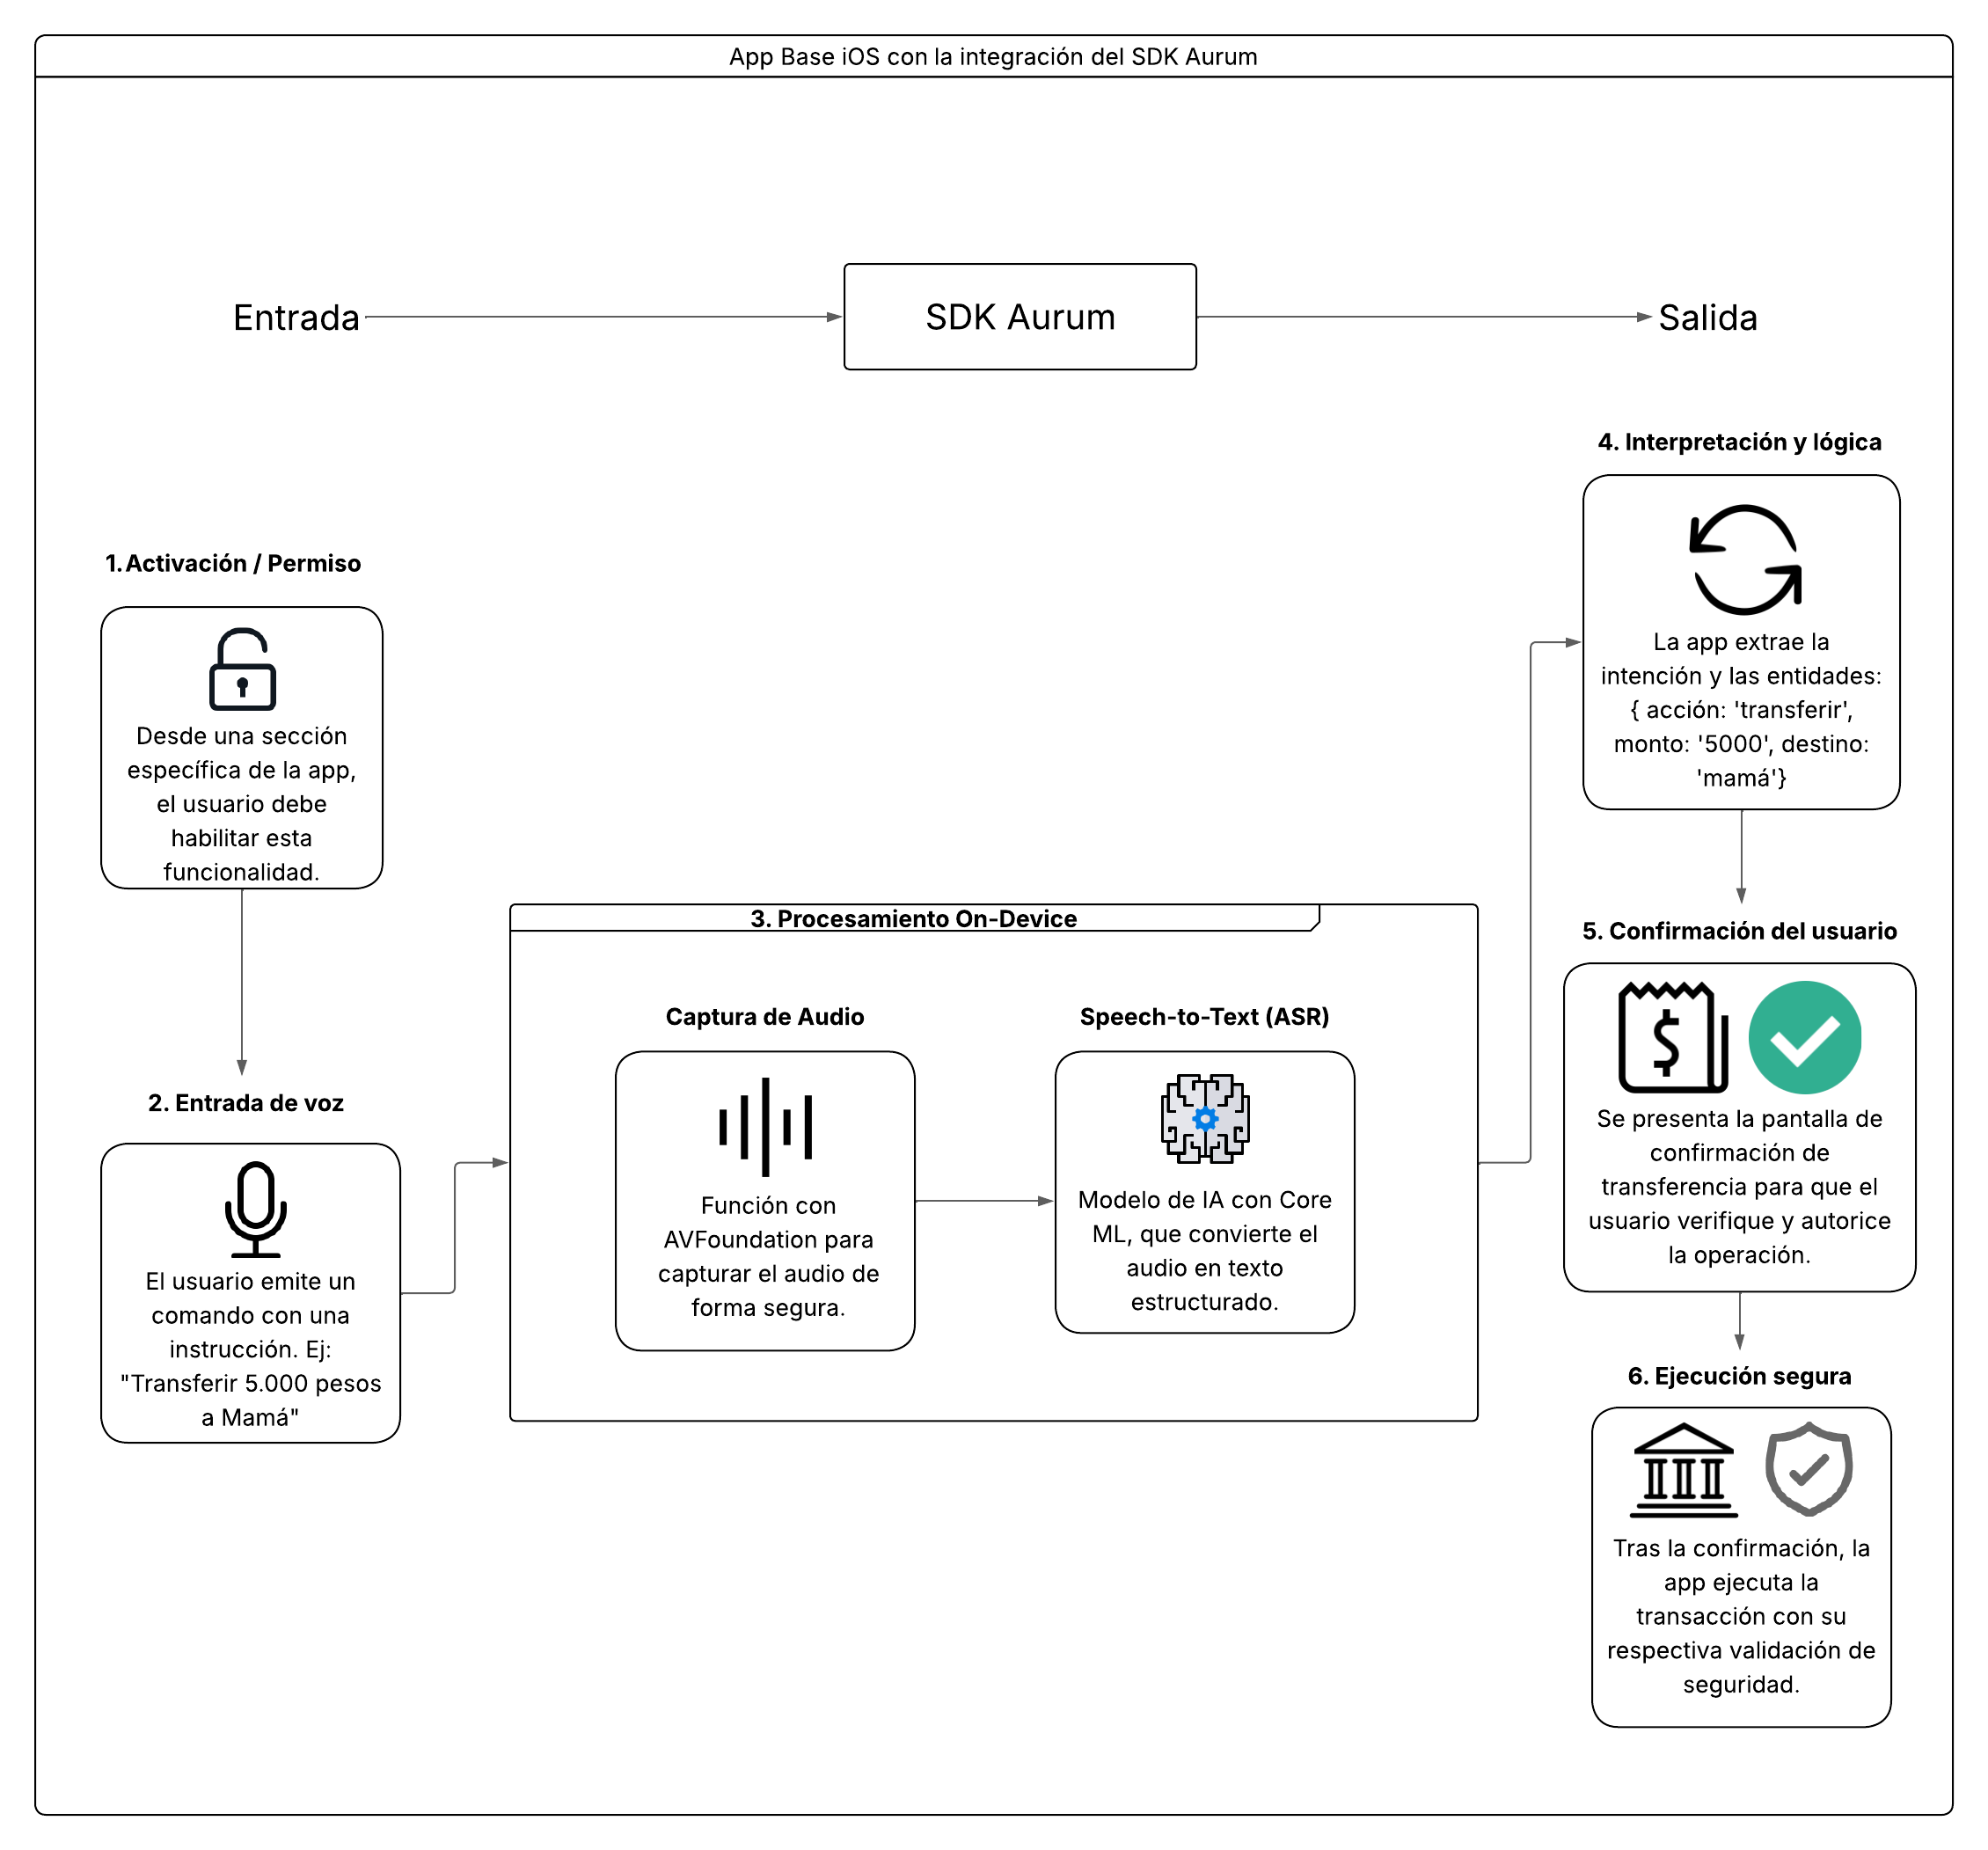
\includegraphics[width=1.0\textwidth]{./Figures/diagrama-de-componentes.png}
\caption{Diagrama de arquitectura de componentes que conforman la prueba de concepto.}
\label{fig:diagComp}
\end{figure}

El ciclo de vida de una transacción impulsada por voz atraviesa un pipeline determinista que fluye secuencialmente a través de las capas de la arquitectura descrita. El proceso de ingesta de datos se desencadena en la aplicación base cuando el usuario, luego de superar los controles de acceso convencionales del banco, interactúa con el disparador de la interfaz gráfica (botón de dictado). En ese instante, la aplicación anfitriona invoca la API pública del SDK Aurum, transfiriéndole el control del hilo de ejecución de audio. El SDK inicializa una sesión de captura de alto rendimiento mediante el framework AVFoundation, configurando el entorno acústico adecuado para aislar la frecuencia de la voz humana.
Una vez digitalizada la señal de audio, el motor interno del SDK emplea las capacidades de transcripción fuera de línea (offline) provistas por las librerías nativas de iOS para ejecutar el reconocimiento automático de habla, esto convierte el espectrograma en una cadena de texto cruda. Acto seguido, este texto es sometido a técnicas de normalización morfológica y es inyectado en el motor de comprensión del lenguaje natural. En esta fase de inferencia, la transcripción es procesada localmente por los modelos vectoriales preentrenados y cuantizados alojados en Core ML. Dichos modelos resuelven algorítmicamente el problema de clasificación de la intención del usuario y proceden al etiquetado posicional para extraer las variables nominales del comando.
El flujo de información concluye cuando la salida matricial de las redes neuronales es traducida por el SDK en un payload \citep{sommerville2015software} de datos estructurado y fuertemente tipado. Este artefacto resultante, que encapsula inequívocamente la acción solicitada, la magnitud numérica del monto, el tipo de divisa y la identidad del beneficiario, es retornado de manera asíncrona a la aplicación anfitriona a través de patrones de delegación (\textit{Delegates o Closures})\citep{apple2026swiftlanguage}. A partir de la entrega de este objeto estructurado, el SDK Aurum finaliza su intervención y cede nuevamente el control a la aplicación base que asume la responsabilidad de mapear el payload contra su modelo de datos transaccional, renderizar la interfaz de validación final ante el usuario y proceder con la comunicación cifrada hacia el core bancario.

En la figura \ref{fig:pipelineVoz} se muestra el flujo del pipeline (ciclo de vida de una transacción por voz).

\begin{figure}[htpb]
\centering 
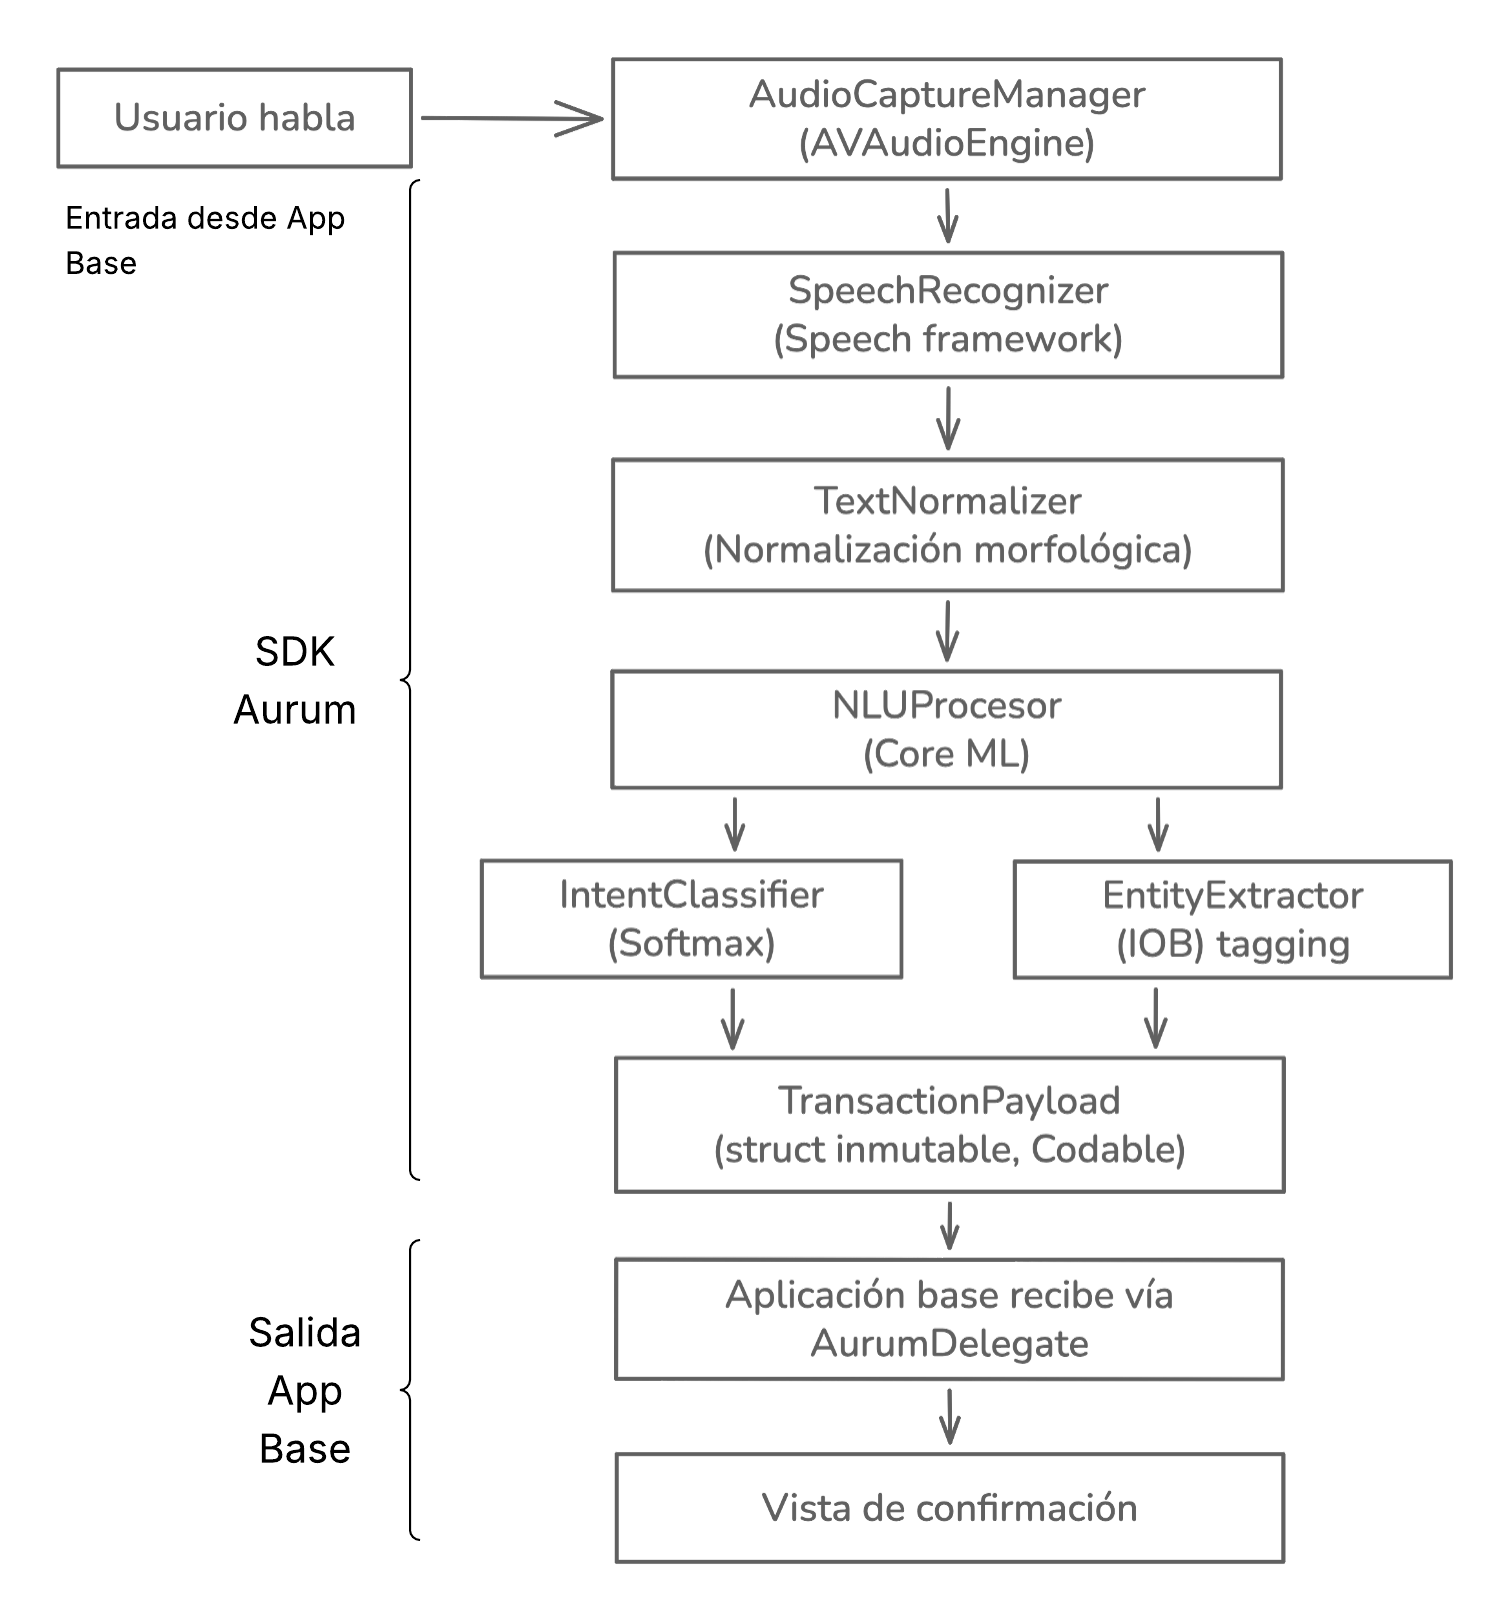
\includegraphics[width=1.0\textwidth]{./Figures/pipeline-transaccion.png}
\vspace{0.5cm} 
\caption{Flujo de pipeline de una transacción realizada por voz.}
\label{fig:pipelineVoz}
\end{figure}

\section{Tratamiento y preparación de datos}

El desarrollo de modelos de procesamiento de lenguaje natural aplicados a dominios de misión crítica, como el sector bancario, enfrenta el desafío inherente del acceso a la información, conocido como el problema de arranque en frío \ (\textit{cold start}). Las estrictas normativas de privacidad y el secreto bancario imposibilitan el uso de corpus conversacionales de clientes reales sin someterlos previamente a procesos de anonimización complejos y costosos. Adicionalmente, al tratarse de una prueba de concepto que introduce un canal de interacción inédito en el entorno simulado de la aplicación móvil, no existe telemetría histórica ni registros acústicos o textuales previos de comandos transaccionales.
Ante esta restricción, se determinó como exigencia metodológica la generación de un conjunto de datos sintéticos (\textit{mock data}). La construcción de un corpus artificial permite no solo superar la ausencia de datos iniciales, sino también ejercer un control riguroso sobre la distribución probabilística de las clases (intenciones) y garantizar una cobertura exhaustiva de los casos límite (\textit{edge cases}) de las entidades. Este enfoque metodológico aísla el desarrollo algorítmico de los riesgos de privacidad y provee un entorno determinista, fundamental para iterar la arquitectura de la red neuronal durante las primeras fases de evaluación.


\subsection {Creación de plantillas de comandos y aumentación de datos}

La síntesis del corpus de entrenamiento se estructuró a partir de la definición de plantillas (\textit{templates}) gramaticales. Estas plantillas modelan lógicamente las posibles estructuras sintácticas que un usuario emplearía para interactuar con el sistema bancario y se abstraen los valores concretos, tales como: [ACCIÓN] [MONTO] [MONEDA] a [DESTINATARIO].
Una vez consolidadas las estructuras base, se implementaron técnicas de aumentación de datos (\textit{data augmentation}) para inyectar la variabilidad inherente al lenguaje natural \cite{feng2021survey}.

La transición entre el entorno probabilístico inherente a los modelos de machine learning y el rigor determinista exigido por los sistemas financieros requiere de una capa de abstracción robusta. Para resolver este paradigma, se estructuraron los datos resultantes de la inferencia algorítmica utilizando estructuras de valor \textit{struct} en Swift  \citep{apple2026swiftlanguage}. El uso de \textit{structs} garantizó la inmutabilidad de la información una vez extraída y procesada, esto prevee alteraciones accidentales de las variables en la memoria durante el ciclo de vida de la transacción.
Para la serialización de este modelo, se adoptó el protocolo Codable nativo de Apple \citep{apple2026codable}. Esta decisión arquitectónica se justificó en la necesidad de estandarizar la comunicación entre el SDK y la aplicación base, así el objeto Swift generado en memoria puede ser codificado y decodificado de manera nativa hacia formatos universales de intercambio de datos, como JSON \citep{rfc8259json}, sin depender de librerías de terceros.

\subsection{Modelo de datos}

El diseño del payload (o carga útil) que el modelo de etiquetado de secuencias (NER) y el clasificador de intenciones devolvieron al sistema se consolidó en una única entidad semántica. Durante el desarrollo, se definieron campos fuertemente tipados para encapsular de manera exacta las variables transaccionales críticas:

\begin{itemize}
	\item Intención: representa la acción directiva inferida del comando verbal (por ejemplo, iniciar una transferencia). Se estructuró como el eje central que define el ruteo posterior dentro de la aplicación.
	\item Monto: se tipificó mediante el uso de datos de punto flotante de doble precisión (\textit{Double}) \citep{apple2026swiftlanguage}, esto permite la representación matemática de la magnitud monetaria extraída de la transcripción fonética.
	\item Moneda: se modeló utilizando enumeraciones (\textit{Enum}) con tipos crudos de cadena de texto (\textit{String raw values}) \citep{apple2026swiftlanguage}. Esto restringió el dominio de la divisa a valores finitos y normalizados bajo estándares internacionales (ej. ARS o USD), eliminando la ambigüedad de sinónimos coloquiales capturados por el motor NLU, como "pesos", "lucas"\ o "dólares".
	\item Destinatario: se definió como una cadena de caracteres cruda (\textit{String}) \citep{apple2026swiftlanguage} que encapsula la identidad nominal del beneficiario de la operación, dejando el valor preparado para ser contrastado posteriormente contra la agenda de contactos o base de alias validada del banco.
\end{itemize}

Este enfoque de modelado determinista cumple una función vital en la arquitectura de integración del sistema. Al transformar una emisión acústica originalmente desestructurada en un objeto Swift predecible y validado a nivel de compilador, se abstrajo a la aplicación anfitriona de toda la complejidad inherente al procesamiento de lenguaje natural. En consecuencia, la integración con los servicios de backend del banco se facilita de manera significativa: la aplicación móvil anfitriona consume un payload limpio, cuya estructura es análoga a la que generaría una interfaz táctil tradicional basada en formularios. Esto habilita a la aplicación base a tomar dichas variables tipadas e inyectarlas de manera directa en los constructores de sus peticiones de red seguras, esto mantendría intacta la lógica de consumo de los endpoints transaccionales de la institución.

\section{Desarrollo del SDK (Aurum)}

El desarrollo de Aurum se abordó bajo el paradigma de la programación orientada a componentes y se materializó como un \textit{framework} dinámico reutilizable dentro del ecosistema de Apple. El propósito fundamental de este encapsulamiento fue abstraer la complejidad algorítmica inherente al procesamiento de señales acústicas y a la inferencia de modelos de \textit{machine learning}, proporcionando a la aplicación bancaria anfitriona una interfaz programática mínima que oculta la totalidad de las operaciones internas. Al aislar el \textit{pipeline} de inteligencia artificial en un módulo independiente, se garantizó la cohesión del código, se facilitó su distribución y mantenimiento futuro, y se evitó la contaminación de la lógica de negocio y de la interfaz de usuario de la aplicación consumidora.

La arquitectura interna del SDK se organiza en cinco componentes especializados, cada uno con una responsabilidad bien delimitada, que se ejecutan de forma secuencial y coordinada bajo la orquestación de una clase fachada principal. La tabla~\ref{tab:componentes-sdk} presenta un resumen de estos componentes y sus dependencias de frameworks nativos de Apple.

Las secciones siguientes describen el diseño e implementación de cada componente, así como la API pública expuesta a la aplicación consumidora.

\begin{table}[htbp]
\centering
% Cambiamos la última 'l' por 'p{4.5cm}' (puedes ajustar el 4.5cm según necesites)
\begin{tabular}{@{} p{3.0cm} p{3.0cm} p{2.5cm} p{4.5cm} @{}}
\toprule
\textbf{Componente} & \textbf{Clase} & \textbf{Framework} & \textbf{Responsabilidad} \\
\midrule
Fachada principal
    & \lstinline|AurumEngine|
    & ---
    & Orquestación del pipeline \\
Captura de audio
    & \lstinline|AudioCaptureManager|
    & AVFoundation
    & Configuración de sesión y captura de buffers \\
Reconocimiento de voz
    & \lstinline|SpeechRecognizer|
    & Speech
    & Transcripción \textit{on-device} \\
Normalización de texto
    & \lstinline|TextNormalizer|
    & Foundation
    & Conversión léxica y numérica \\
Procesamiento NLU
    & \lstinline|NLUProcessor|
    & \lstinline|NaturalLanguage, CoreML|
    & Clasificación de intención y extracción de entidades \\
\bottomrule
\end{tabular}
\caption{Componentes del SDK Aurum y sus dependencias de frameworks nativos.}
\label{tab:componentes-sdk}
\end{table}


\subsection{Clase fachada: \texttt{AurumEngine}}

Para orquestar la ejecución secuencial de las etapas de procesamiento, se implementó la clase \texttt{AurumEngine} siguiendo el patrón de diseño
\textit{Facade} \citep{gamma1994design}. Esta clase constituye el único punto de entrada público del SDK y su responsabilidad es coordinar el ciclo de vida integral de la transacción de voz: desde la activación del micrófono hasta la entrega del \texttt{TransactionPayload} resultante.

Internamente, \texttt{AurumEngine} mantiene referencias privadas a los cuatro componentes de procesamiento y los instancia durante la fase de configuración. La API pública expone únicamente tres métodos de control:

\begin{lstlisting}[caption={API pública de \texttt{AurumEngine}.},label={lst:aurum-engine}]
public class AurumEngine {

    public weak var delegate: AurumDelegate?

    private let audioManager = AudioCaptureManager()
    private let speechRecognizer = SpeechRecognizer()
    private let textNormalizer = TextNormalizer()
    private let nluProcessor = NLUProcessor()

    /// Precarga los modelos Core ML desde el bundle de la app.
    public func configure(bundle: Bundle) {
        nluProcessor.loadModels(from: bundle)
    }

    /// Inicia la captura de audio y el reconocimiento de voz.
    public func startListening() { /* ... */ }

    /// Detiene la captura y fuerza el procesamiento del texto acumulado.
    public func stopListening() { /* ... */ }

    /// Cancela la operacion en curso y libera recursos.
    public func cancelListening() { /* ... */ }
}
\end{lstlisting}


El método \texttt{configure(bundle:)} recibe el \texttt{Bundle} de la aplicación anfitriona para localizar los archivos \texttt{.mlmodelc} compilados
(\texttt{IntentClassifier} y \texttt{EntityExtractor}) e instanciar los objetos \texttt{NLModel} correspondientes. Esta precarga se ejecuta una única vez
durante el inicio de la aplicación y permite que las inferencias posteriores se resuelvan con latencia mínima, evitando el costo de carga en caliente
(\textit{cold start}) durante la interacción de voz.


\subsection{Captura de audio: \texttt{AudioCaptureManager}}

El primer eslabón del pipeline es la gestión del hardware de audio del dispositivo. El componente \texttt{AudioCaptureManager} encapsula la
interacción con los frameworks \texttt{AVAudioSession} y \texttt{AVAudioEngine} de Apple, y resuelve tres tareas técnicas:

\begin{enumerate}
    \item Solicitud de permisos: la primera invocación verifica el estado de autorización del micrófono mediante
    \texttt{AVAudioSession.recordPermission}. Si el permiso no fue concedido previamente, dispara la solicitud nativa del sistema operativo. En caso de
    denegación, el componente reporta un error tipado (\texttt{AurumError.microphonePermissionDenied}) sin intentar activar la
    captura.

    \item Configuración de la sesión de audio: se establece la categoría \texttt{.playAnd\linebreak Record} con modo \texttt{.measurement}. La
    categoría \texttt{.playAndRecord} permite la entrada y salida simultánea de audio (necesaria para dispositivos con altavoz activo), mientras que el modo \texttt{.measurement} desactiva los filtros de ecualización y cancelación de ruido del sistema, proporcionando una señal de audio cruda óptima para
    el reconocedor de voz.

    \item Instalación del \textit{tap} de audio: se accede al nodo de  entrada (\texttt{inputNode}) del \texttt{AVAudioEngine} y se instala un
    \textit{tap} que captura \textit{buffers} de audio en formato PCM a la frecuencia de muestreo nativa del micrófono (típicamente 44.1~kHz o
    48~kHz). Estos \textit{buffers} se canalizan al componente \texttt{Speech\linebreak Recognizer} mediante un cierre (\textit{closure}).
\end{enumerate}

\begin{lstlisting}[caption={Configuración de la sesión de audio y captura de \textit{buffers}.},label={lst:audio-capture}]
func startCapture(onBuffer: @escaping (AVAudioPCMBuffer) -> Void) throws {
    let session = AVAudioSession.sharedInstance()
    try session.setCategory(.playAndRecord, mode: .measurement,
                            options: [.defaultToSpeaker])
    try session.setActive(true)

    let inputNode = audioEngine.inputNode
    let format = inputNode.outputFormat(forBus: 0)

    inputNode.installTap(onBus: 0, bufferSize: 1024, format: format)
    { buffer, _ in
        onBuffer(buffer)
    }

    audioEngine.prepare()
    try audioEngine.start()
}
\end{lstlisting}

La detención de la captura (\texttt{stopCapture()}) remueve el \textit{tap}, detiene el \texttt{AVAudioEngine} y desactiva la sesión de audio, liberando el
hardware del micrófono para que otras aplicaciones puedan utilizarlo.

\subsection{Reconocimiento de voz: \texttt{SpeechRecognizer}} 

El componente \texttt{SpeechRecognizer} integra el \textit{framework} nativo \texttt{Speech} \cite{apple2026speech} para ejecutar la transcripción de voz a texto. Su diseño responde a dos requisitos fundamentales del sistema: el soporte para español rioplatense y la garantía de procesamiento exclusivamente local.

La instanciación del reconocedor se realiza con el \textit{locale} específico \texttt{es-AR} (español de Argentina), lo que activa el modelo acústico y el
modelo de lenguaje optimizados para las particularidades fonéticas y léxicas del habla rioplatense:

\begin{lstlisting}[caption={Configuración del reconocedor de voz con procesamiento \textit{on-device}.},label={lst:speech-recognizer}]
private let recognizer = SFSpeechRecognizer(
    locale: Locale(identifier: "es-AR")
)

func startRecognition(onPartial: @escaping (String) -> Void,
                      onFinal: @escaping (String) -> Void) {
    let request = SFSpeechAudioBufferRecognitionRequest()

    // Forzar procesamiento local: ningun audio sale del dispositivo
    request.requiresOnDeviceRecognition = true

    // Sugerencias contextuales para el dominio financiero
    request.contextualStrings = [
        "transferir", "transferencia", "enviar", "mandar",
        "consultar", "saldo", "cancelar", "anular",
        "pesos", "dolares", "lucas", "verdes", "mangos"
    ]

    recognizer?.recognitionTask(with: request) { result, error in
        guard let result = result else { return }
        let text = result.bestTranscription.formattedString
        if result.isFinal {
            onFinal(text)
        } else {
            onPartial(text)
        }
    }
}
\end{lstlisting}


La propiedad \texttt{requiresOnDeviceRecognition = true} es la piedra angular de la estrategia de privacidad del sistema. Esta configuración instruye al
\textit{Speech Framework} a utilizar exclusivamente el modelo de reconocimiento descargado localmente en el dispositivo, bloqueando cualquier transmisión de paquetes de audio a los servidores de Apple. Si el modelo local no se encuentra disponible (por ejemplo, porque el usuario no descargó el paquete de idioma texttt{es-AR} para uso sin conexión), el reconocedor reporta un error en lugar de recurrir silenciosamente al procesamiento en la nube.

La propiedad \texttt{contextualStrings} proporciona al motor de reconocimiento un vocabulario de refuerzo específico del dominio financiero. Al incluir
términos como ``transferencia'', ``saldo'' o ``lucas'', se incrementa la probabilidad de que el reconocedor transcriba correctamente estas palabras
frente a alternativas fonéticamente similares pero semánticamente irrelevantes. Este mecanismo de \textit{biasing} léxico no modifica el modelo acústico
subyacente, sino que ajusta las probabilidades del modelo de lenguaje durante la decodificación.

El reconocimiento opera en modo \textit{streaming}: a medida que el usuario habla, el \textit{framework} genera hipótesis parciales que se entregan
progresivamente al delegado de la app para su visualización en tiempo real. Cuando el motor detecta una pausa prolongada o el final del enunciado, emite el resultado final (\texttt{result.isFinal = true}) que constituye la entrada para la etapa de normalización.


\subsection{Normalización de texto: \texttt{TextNormalizer}} 

La transcripción cruda del reconocedor de voz contiene frecuentemente expresiones coloquiales, numéricas y morfológicas que no pueden ser procesadas directamente por los modelos de clasificación e extracción de entidades. El componente \texttt{TextNormalizer} actúa como capa intermedia de limpieza y estandarización, transformando el texto transcrito en una forma canónica compatible con el vocabulario del corpus de entrenamiento.

Las transformaciones implementadas abarcan tres categorías:

\subsubsection*{Conversión de expresiones numéricas}

El normalizador convierte las representaciones textuales de números a su forma numérica. Esta conversión abarca tanto las formas estándar del español
(``quinientos'' $\rightarrow$ 500, ``mil'' $\rightarrow$ 1000, ``doscientos cincuenta'' $\rightarrow$ 250) como las expresiones coloquiales rioplatenses
que involucran multiplicadores implícitos.

\subsubsection*{Normalización de léxico coloquial}

El habla rioplatense utiliza un conjunto de términos coloquiales para referirse a monedas y denominaciones que no forman parte del vocabulario financiero formal. El normalizador mantiene un diccionario de equivalencias que mapea estas expresiones a sus formas canónicas:

\begin{lstlisting}[caption={Diccionario de normalización para léxico coloquial rioplatense.},label={lst:normalizer}]
private let colloquialMap: [String: (canonical: String, multiplier: Double?)] = [
    // Denominaciones de moneda
    "lucas":  (canonical: "pesos",   multiplier: 1000),
    "luca":   (canonical: "pesos",   multiplier: 1000),
    "mangos": (canonical: "pesos",   multiplier: nil),
    "guita":  (canonical: "pesos",   multiplier: nil),
    "verdes": (canonical: "dolares", multiplier: nil),

    // Expresiones de cantidad
    "palo":   (canonical: "pesos",   multiplier: 1_000_000),
    "gambas": (canonical: "pesos",   multiplier: 100),
]
\end{lstlisting}

Cuando el normalizador encuentra la expresión ``dos lucas'', la resuelve como \texttt{2 $\times$ 1000 = 2000 pesos}: el numeral ``dos'' se convierte a su
valor numérico, el término ``lucas'' aporta la moneda canónica (``pesos'') y el multiplicador ($\times 1000$). Análogamente, ``cinco gambas'' se transforma en \texttt{5 $\times$ 100 = 500 pesos}, y ``medio palo'' en \texttt{0.5 $\times$ 1\,000\,000 = 500\,000 pesos}.

\subsubsection*{Normalización morfológica}

Esta categoría comprende la conversión de formas verbales del voseo rioplatense a sus formas imperativas estándar (``transferí'' $\rightarrow$ ``transferir'', ``fijate'' $\rightarrow$ ``consultar'') y la eliminación de partículas coloquiales que no aportan contenido semántico (``che'', ``dale'', ``na'',
``bueno''). Estas transformaciones reducen la variabilidad léxica de la entrada y mejoran la probabilidad de que los modelos clasifiquen correctamente la
intención, dado que el corpus de entrenamiento incluye predominantemente formas canónicas.


\subsection{Procesamiento NLU: \texttt{NLUProcessor}}

El componente \texttt{NLUProcessor} constituye el núcleo de inteligencia artificial del SDK. Su responsabilidad es resolver el problema dual de
clasificación de intenciones y extracción de entidades nombradas (NER) a partir del texto normalizado, utilizando los modelos Core~ML entrenados con el
\textit{framework} Create~ML.

La arquitectura del procesador se basa en las clases \texttt{NLModel} y \texttt{NLTagger} del framework \texttt{NaturalLanguage} de Apple \citep{apple-naturallanguage}, que proporcionan una interfaz de alto nivel para la inferencia de modelos compilados en formato \texttt{.mlmodelc}.

\subsubsection{Clasificación de intenciones}

La clasificación de intenciones determina cuál de las tres operaciones transaccionales soportadas corresponde al comando de voz del usuario. El
modelo \texttt{Intent\linebreak Classifier}, entrenado con el algoritmo \textit{Maximum Entropy} (MaxEnt), se carga como instancia de \texttt{NLModel}
y expone un método de predicción que recibe un \textit{string} y retorna la etiqueta de clase con mayor probabilidad junto con su nivel de confianza:

\begin{lstlisting}[caption={Clasificación de intención con umbral de confianza.},label={lst:intent-classification}]
private var intentModel: NLModel?

func classifyIntent(_ text: String) -> (TransactionIntent, Float) {
    guard let model = intentModel else {
        return (.desconocida, 0.0)
    }

    let hypotheses = model.predictedLabelHypotheses(
        for: text, maximumCount: 3
    )

    guard let topLabel = model.predictedLabel(for: text),
          let confidence = hypotheses[topLabel] else {
        return (.desconocida, 0.0)
    }

    // Aplicar umbral de confianza
    guard confidence >= intentConfidenceThreshold else {
        return (.desconocida, Float(confidence))
    }

    let intent = TransactionIntent(rawValue: topLabel) ?? .desconocida
    return (intent, Float(confidence))
}
\end{lstlisting}


El umbral de confianza (\texttt{intentConfidenceThreshold = 0.65}) actúa como mecanismo de seguridad: si ninguna de las tres clases alcanza este valor, el procesador asigna la intención \texttt{.desconocida}, lo que evita que el sistema ejecute una operación financiera basada en una clasificación incierta. El valor de 0.65 fue seleccionado empíricamente como punto de equilibrio entre la tasa de rechazo de comandos legítimos (\textit{false negatives}) y la aceptación errónea de comandos ambiguos (\textit{false positives}).

Las tres intenciones soportadas se modelan mediante un enumerado tipado:

\begin{lstlisting}[caption={Enumerado de intenciones transaccionales.},label={lst:intent-enum}]
enum TransactionIntent: String, Codable {
    case transferencia  = "TRANSFERENCIA"
    case consultaSaldo  = "CONSULTA_SALDO"
    case cancelar       = "CANCELAR"
    case desconocida    = "DESCONOCIDA"

    var requiresEntityExtraction: Bool {
        switch self {
        case .transferencia: return true
        case .consultaSaldo, .cancelar, .desconocida: return false
        }
    }
}
\end{lstlisting}

La propiedad computada \texttt{requiresEntityExtraction} permite optimizar el pipeline: si la intención detectada es \texttt{.consultaSaldo} o
\texttt{.cancelar}, se omite la etapa de extracción de entidades (que solo es relevante para transferencias), reduciendo la latencia total del procesamiento.


\subsubsection{Extracción de entidades nombradas (NER)}

Para las intenciones de tipo \texttt{.transferencia}, el procesador activa la extracción de entidades nombradas utilizando el modelo \texttt{EntityExtractor}, entrenado con el algoritmo \textit{Conditional Random Field} (CRF). Este modelo, cargado en un \texttt{NLTagger}, etiqueta cada
token del texto normalizado con una de las siete clases del esquema IOB definido: \texttt{B-MONTO}, \texttt{I-MONTO},
\texttt{B-MONEDA}, \texttt{I-MONEDA}, \texttt{B-DESTINATARIO}, \texttt{I-DESTINATARIO} y \texttt{O} (\textit{Outside}).

\begin{lstlisting}[caption={Extracción de entidades con \texttt{NLTagger} y esquema IOB.},label={lst:ner-extraction}]
private var entityTagger: NLTagger?

func extractEntities(_ text: String) -> (Double?, Currency?, String?) {
    guard let tagger = entityTagger else { return (nil, nil, nil) }

    tagger.string = text
    var currentEntity: String? = nil
    var entityTokens: [String: [String]] = [:]

    tagger.enumerateTags(
        in: text.startIndex..<text.endIndex,
        unit: .word,
        scheme: .nameType,
        options: [.omitWhitespace, .omitPunctuation]
    ) { tag, range in
        let token = String(text[range])
        let label = tag?.rawValue ?? "O"

        if label.hasPrefix("B-") {
            currentEntity = String(label.dropFirst(2))
            entityTokens[currentEntity!, default: []].append(token)
        } else if label.hasPrefix("I-"), let entity = currentEntity {
            entityTokens[entity, default: []].append(token)
        } else {
            currentEntity = nil
        }
        return true
    }

    // Reconstruir valores tipados
    let amount = parseAmount(entityTokens["MONTO"])
    let currency = Currency.fromTokens(entityTokens["MONEDA"])
    let recipient = entityTokens["DESTINATARIO"]?.joined(separator: " ")

    return (amount, currency, recipient)
}
\end{lstlisting}

La reconstrucción de entidades a partir de las etiquetas IOB sigue un algoritmo lineal: al encontrar una etiqueta \texttt{B-X} se inicia una nueva entidad de tipo \texttt{X}; las etiquetas \texttt{I-X} consecutivas extienden la entidad actual; cualquier otra etiqueta cierra la entidad en curso. Este esquema
permite capturar entidades de longitud variable, como nombres compuestos (``Juan Pérez'' = \texttt{B-DESTINATARIO} + \texttt{I-DESTINATARIO}) o montos con modificadores (``dos mil quinientos'' = \texttt{B-MONTO} + \texttt{I-MONTO} + \texttt{I-MONTO}).

Las tres entidades extraídas se tipan mediante las estructuras de datos del SDK: \texttt{MONTO} se convierte a \texttt{Double}, \texttt{MONEDA} se mapea al enumerado \texttt{Currency} (que soporta las variantes coloquiales mediante el método estático \texttt{fromColloquial}), y \texttt{DESTINATARIO} se reconstruye como \texttt{String} concatenando los tokens etiquetados.


\subsection{Modelo de datos: \texttt{TransactionPayload}} 

El resultado consolidado del pipeline se encapsula en la estructura \texttt{Transaction\linebreak Payload}, un \textit{value type} inmutable que adopta los
protocolos \texttt{Codable} y \linebreak \texttt{Equatable} de Swift:

\begin{lstlisting}[caption={Estructura del \textit{payload} de transacción.},label={lst:payload}]
struct TransactionPayload: Codable, Equatable {
    let intent: TransactionIntent
    let amount: Double?
    let currency: Currency?
    let recipient: String?
    let rawTranscription: String
    let intentConfidence: Float
    let timestamp: Date
}
\end{lstlisting}

La elección de una \texttt{struct} (tipo por valor) en lugar de una texttt{class} (tipo por referencia) es deliberada: al ser inmutable y copiarse por valor, el \textit{payload} no puede ser modificado accidentalmente por la aplicación consumidora tras su recepción. Los campos \texttt{amount}, \texttt{currency} y \texttt{recipient} son opcionales (\texttt{Optional}) porque no todas las intenciones requieren entidades: una consulta de saldo no
tiene monto ni destinatario.

La adopción del protocolo \texttt{Codable} permite serializar el \textit{payload} a JSON con una única invocación (\texttt{JSONEncoder().encode(payload)}), lo que facilita su transmisión a un \textit{backend} bancario en una mplementación productiva. El protocolo \texttt{Equatable} habilita las comparaciones por valor, útiles para las pruebas unitarias del SDK.


\subsection{API pública y comunicación asíncrona} 

Dado que la captura de audio y la inferencia neuronal son procesos no bloqueantes que se ejecutan en hilos de trabajo (\textit{background threads}),
la comunicación entre el SDK y la aplicación anfitriona se resolvió mediante el patrón \textit{Delegate} de Cocoa \citep{apple-delegation}. Este patrón
define un protocolo formal que la aplicación consumidora implementa para recibir notificaciones asíncronas sobre los eventos del pipeline:

\begin{lstlisting}[caption={Protocolo \texttt{AurumDelegate}: canal de comunicación asíncrona del SDK.},label={lst:delegate-protocol}]
protocol AurumDelegate: AnyObject {

    /// El SDK activo el microfono y comenzo a capturar audio.
    func aurumDidStartListening()

    /// El SDK detuvo la captura de audio.
    func aurumDidStopListening()

    /// Nueva hipotesis parcial de transcripcion disponible.
    func aurumDidReceivePartialTranscription(_ text: String)

    /// El pipeline completo exitosamente. Entrega el payload.
    func aurumDidCompleteWithPayload(_ payload: TransactionPayload)

    /// Ocurrio un error en alguna etapa del pipeline.
    func aurumDidFailWithError(_ error: AurumError)
}
\end{lstlisting}

El protocolo extiende \texttt{AnyObject}, lo que restringe su adopción a tipos por referencia (\textit{classes}). Esto permite que \texttt{AurumEngine}
mantenga una referencia débil (\texttt{weak var delegate}) al delegado, evitando ciclos de retención de memoria (\textit{retain cycles}) que podrían
provocar \textit{memory leaks} en la aplicación.

Los cinco \textit{callbacks} del delegado cubren la totalidad del ciclo de vida de una transacción de voz. El \textit{callback}
\texttt{aurumDidReceivePartialTranscription(\_:)} es particularmente relevante desde la perspectiva de la experiencia de usuario: al entregar hipótesis
parciales de transcripción en tiempo real, la aplicación puede proporcionar retroalimentación visual inmediata que confirma al usuario que el sistema está procesando su voz.


\subsection{Gestión de errores: \texttt{AurumError}} 

El SDK define un enumerado de errores tipados que cubre los modos de fallo de cada etapa del pipeline. Al utilizar un tipo enumerado en lugar de errores genéricos, la aplicación consumidora puede implementar manejo diferenciado según la naturaleza del fallo:

\begin{lstlisting}[caption={Enumerado de errores tipados del SDK.},label={lst:errors}]
enum AurumError: Error, LocalizedError {
    case microphonePermissionDenied
    case speechRecognitionDenied
    case speechRecognizerUnavailable
    case audioSessionConfigurationFailed(underlying: Error)
    case speechRecognitionFailed(underlying: Error)
    case nluModelLoadFailed(modelName: String)
    case nluInferenceFailed(underlying: Error)
    case payloadValidationFailed(reason: String)

    var errorDescription: String? {
        switch self {
        case .microphonePermissionDenied:
            return "Permiso de microfono denegado."
        case .speechRecognitionDenied:
            return "Permiso de reconocimiento de voz denegado."
        case .speechRecognizerUnavailable:
            return "Reconocedor de voz no disponible para es-AR."
        case .audioSessionConfigurationFailed(let e):
            return "Error de configuracion de audio: \(e.localizedDescription)"
        case .speechRecognitionFailed(let e):
            return "Error de reconocimiento: \(e.localizedDescription)"
        case .nluModelLoadFailed(let name):
            return "No se pudo cargar el modelo: \(name)"
        case .nluInferenceFailed(let e):
            return "Error de inferencia NLU: \(e.localizedDescription)"
        case .payloadValidationFailed(let reason):
            return "Payload invalido: \(reason)"
        }
    }
}
\end{lstlisting}

Los errores que envuelven un error subyacente (\texttt{underlying: Error}) preservan la cadena de causalidad, lo que facilita el diagnóstico durante el
desarrollo. Por ejemplo, si \texttt{AVAudioSession.setActive()} falla por un conflicto con otra sesión de audio activa, el error subyacente del sistema
operativo queda encapsulado dentro de \texttt{.audioSessionConfigurationFailed} y es accesible para logging sin
exponer detalles internos al usuario final.

\medskip

En síntesis, la arquitectura del SDK Aurum materializa los principios de encapsulamiento, cohesión y mínima superficie de API que guiaron el diseño del
sistema. La aplicación consumidora interactúa exclusivamente con tres métodos públicos (\texttt{startListening}, \texttt{stopListening},
\texttt{cancelListening}) y cinco \textit{callbacks} del delegado, permaneciendo completamente agnóstica respecto a las operaciones de vectorización, etiquetado y transcripción que ocurren internamente. Esta separación de responsabilidades se valida en la sección~\ref{sec:app-base}, donde se describe la integración del SDK en la aplicación base de prueba de concepto.







\begin{comment}
El desarrollo de Aurum se abordó bajo el paradigma de la programación orientada a componentes, se materilizó como un \textit{framework} dinámico y reutilizable dentro del ecosistema de Apple. El propósito fundamental de este encapsulamiento radicó en abstraer la alta complejidad algorítmica inherente al procesamiento de señales acústicas y a la inferencia neuronal, dándole a la aplicación bancaria anfitriona una "caja negra" funcional. Al aislar el pipeline de inteligencia artificial en un módulo independiente, se garantizó la cohesión del código y se facilitó su futura distribución y mantenimiento, sin contaminar la lógica de negocio ni la interfaz de usuario de la aplicación base.
Para orquestar la ejecución secuencial de las tareas de procesamiento, se implementó una clase principal o \textit{facade} (fachada) dentro del SDK, responsable de coordinar el ciclo de vida integral de la transacción de voz. El primer eslabón de esta coordinación consistió en la gestión del hardware de audio del dispositivo. A través de la API AVAudioSession, se configuró el entorno acústico solicitando los permisos de grabación al sistema operativo y lo que establece la categoría de la sesión para priorizar la entrada de voz (record o playAndRecord). Seguidamente, se instanció un AVAudioEngine para capturar el flujo continuo de muestras de audio provenientes del micrófono y canalizarlas hacia los nodos de procesamiento.
Una vez establecido el buffer de audio, la clase principal integró el \textit{framework} nativo Speech \citep{apple2026speech} para ejecutar la transcripción de voz a texto. Para cumplir con las estrictas normativas de privacidad del sector financiero, se forzó el procesamiento estrictamente local configurando la propiedad requiresOnDeviceRecognition en verdadero (true). Esta restricción arquitectónica impidió que los paquetes de audio fueran transmitidos a los servidores en la nube de Apple. Posteriormente, la cadena de texto transcrita fue inyectada en el módulo de comprensión de lenguaje natural. En esta instancia, el SDK invocó los modelos de machine learning, previamente entrenados y cuantizados, a través del \textit{framework} Core ML. La ejecución local de estos modelos permitió clasificar la intención transaccional y extraer las entidades relevantes (monto, moneda, destinatario) con una latencia del orden de los milisegundos, aprovechando la aceleración por hardware del dispositivo.
Para consolidar la integración, el SDK Aurum fue dotado de una Interfaz de Programación de Aplicaciones (API) pública minimalista \citep{ieee1990glossary}. Dado que la captura de audio y la inferencia neuronal son procesos no bloqueantes que ocurren a lo largo del tiempo, la comunicación con la aplicación anfitriona se resolvió utilizando patrones asíncronos nativos de Swift, combinando el uso de delegados ( \textit{Delegates}) y clausuras (\textit{Closures}). De este modo, la aplicación base únicamente necesita invocar un método público de inicio de escucha (por ejemplo, startListening()) y suscribirse para recibir la respuesta. Al finalizar el procesamiento, el SDK ejecuta un callback que retorna el payload de datos estructurado (detallado en la sección anterior) o, en su defecto, un error tipificado. Esta arquitectura basada en eventos asegura que la aplicación consumidora permanezca completamente agnóstica respecto a las operaciones matemáticas de vectorización, etiquetado y transcripción que ocurren bajo la superficie.
\end{comment}



\begin{comment}
Para evaluar la viabilidad de la integración y el correcto funcionamiento del SDK Aurum, se desarrolló una aplicación móvil de prueba que emula el entorno transaccional de una entidad bancaria. Esta aplicación base se construyó con el propósito de actuar como el contenedor cliente que orquesta la experiencia del usuario y consume la API expuesta por el \textit{framework} de procesamiento de lenguaje natural.
El diseño de la interfaz de usuario se estructuró bajo principios de minimalismo y accesibilidad, focalizándose en el flujo de interacción conversacional. En la vista principal, se implementó un botón de activación por voz que actúa como el disparador (\textit{trigger}) del ciclo transaccional. Para proveer una experiencia de usuario coherente y mitigar la incertidumbre del sistema, se diseñó un mecanismo de retroalimentación visual. Durante el estado de escucha, la interfaz modifica dinámicamente su estado gráfico para indicarle al usuario de forma inequívoca que el hardware de audio se encuentra activo, capturando y procesando el comando verbal en tiempo real.
Una vez que el SDK finaliza la inferencia neuronal y la extracción de parámetros, la aplicación anfitriona recibe el payload estructurado de manera asíncrona a través de sus métodos delegados. Este intercambio determinista de datos permite a la aplicación base extraer las variables transaccionales (intención, monto, moneda y destinatario) e inyectarlas directamente en su modelo de vistas. Como resultado de este mapeo, la aplicación renderiza una pantalla de confirmación simulada que expone la información procesada de manera legible y estructurada, brindando al usuario la oportunidad de auditar los datos extraídos de su propia voz antes de autorizar la ejecución de la transferencia.

Finalmente, resulta imperativo reiterar la restricción arquitectónica que rige el diseño de este sistema. En el contexto de esta prueba de concepto, la transacción concluye tras la confirmación en la interfaz gráfica simulada. No obstante, en un entorno productivo real, la aplicación base constituye el único perímetro de seguridad autorizado. Es estrictamente en esta capa superior de la aplicación base donde la entidad financiera ejecutaría sus métodos propietarios de validación de identidad, evaluación de riesgos y autenticación multifactor, tales como la validación biométrica facial o el ingreso de credenciales, de manera previa a la confirmación definitiva de la transacción, asegurando que el SDK Aurum opere exclusivamente como un facilitador de accesibilidad y no como un validador criptográfico.
\end{comment}

\section{Desarrollo de la app base}

Con el objetivo de validar la viabilidad funcional del SDK Aurum en un entorno OS real, se desarrolló una aplicación base que opera como prueba de concepto (\textit{Proof of Concept}, PoC). Esta aplicación no constituye un producto bancario completo, sino el artefacto mínimo necesario para demostrar la ejecución integral del \textit{pipeline} de voz: desde la activación del micrófono por parte del usuario hasta la presentación estructurada del
\texttt{TransactionPayload} resultante en la interfaz gráfica.

La app base cumple un doble propósito dentro de este trabajo. En primer lugar, evidencia que la arquitectura del SDK efectivamente encapsula toda la complejidad del procesamiento de lenguaje natural y que un consumidor externo puede integrarla mediante un protocolo \textit{delegate} sin conocer los detalles internos de la cadena de inferencia. En segundo lugar, proporciona el escenario de ejecución para las mediciones de latencia, \textit{accuracy} y robustez lingüística reportadas en el capítulo de resultados.


\subsection{Arquitectura MVVM y flujo de estados}

La aplicación adopta el patrón arquitectónico \textit{Model-View-ViewModel} (MVVM), que es el paradigma idiomático recomendado por Apple para aplicaciones construidas con SwiftUI \cite{apple-swiftui}. En este patrón, la vista (\textit{View}) se limita a declarar la estructura visual de la interfaz de
manera reactiva; el modelo de vista (\textit{ViewModel}) centraliza el estado mutable y la lógica de presentación; y el modelo (\textit{Model}) representa
los datos de dominio, en este caso, el \texttt{TransactionPayload} generado por el SDK.

La elección de MVVM responde a dos consideraciones técnicas. Primero, SwiftUI implementa un mecanismo de enlace de datos (\textit{data binding}) basado en el protocolo \texttt{ObservableObject} y el \textit{property wrapper} \texttt{@Published}: cuando una propiedad marcada como \texttt{@Published} muta su valor, el framework invalida automáticamente las vistas que la observan y las redibuja. Esto elimina la necesidad de gestionar manualmente la sincronización entre estado y presentación, reduce la superficie de errores y produce un código declarativo que refleja directamente el diseño de la interacción. Segundo, MVVM desacopla la lógica de negocio de la capa visual, lo que facilita las pruebas unitarias del \textit{ViewModel} sin necesidad de instanciar componentes gráficos.

El componente central de la arquitectura es la clase \texttt{TransactionViewModel}, que implementa \texttt{ObservableObject} y
adopta el protocolo \texttt{AurumDelegate} definido por el SDK. Su responsabilidad principal es modelar una máquina de estados finita que gobierna
la transición entre las distintas fases de la interacción de voz. El enum \texttt{ViewState} define los estados posibles:

\begin{lstlisting}[caption={Definición de los estados de la interfaz en \texttt{TransactionViewModel}.},label={lst:viewstate}]
enum ViewState {
    case idle           // Esperando activacion del usuario
    case listening      // Microfono activo, capturando audio
    case processing     // Texto recibido, ejecutando NLU
    case confirmation   // Payload listo, esperando confirmacion
    case error          // Error recuperable en cualquier etapa
}
\end{lstlisting}

Las transiciones entre estados se disparan exclusivamente por los \textit{callbacks} del protocolo \texttt{AurumDelegate}, lo que garantiza que
el \textit{ViewModel} nunca manipula directamente los componentes de reconocimiento de voz ni de inferencia. Las transiciones válidas son las
siguientes:

\begin{itemize}
    \item \texttt{idle} $\rightarrow$ \texttt{listening}: el usuario presiona el botón de micrófono y el SDK confirma la activación mediante \texttt{aurumDidStartListening()}.
    \item \texttt{listening} $\rightarrow$ \texttt{processing}: el SDK detecta el fin de habla, invoca \linebreak \texttt{aurumDidStopListening()} e inicia el procesamiento NLU internamente.
    \item \texttt{processing} $\rightarrow$ \texttt{confirmation}: el SDK completa la inferencia y entrega el \texttt{TransactionPayload} vía \texttt{aurumDidCompleteWithPayload(\_:)}.
    \item \texttt{processing} $\rightarrow$ \texttt{error}: ocurre un fallo durante la inferencia, notificado mediante \texttt{aurumDidFailWithError(\_:)}.
    \item \texttt{listening} $\rightarrow$ \texttt{error}: el reconocedor de voz falla (por ejemplo, por interferencia de audio o desconexión del micrófono).
    \item \texttt{confirmation} $\rightarrow$ \texttt{idle}: el usuario confirma o cancela la transacción, reseteando el ciclo.
    \item \texttt{error} $\rightarrow$ \texttt{idle}: el usuario descarta el error y retorna al estado inicial.
\end{itemize}


\subsection{Integración con el SDK Aurum}

La integración entre la app base y el SDK Aurum se realiza exclusivamente a través de dos puntos de contacto: la clase pública \texttt{AurumEngine} (como fachada de control) y el protocolo \texttt{AurumDelegate} (como canal de notificaciones asíncronas). Este diseño materializa el principio de inversión de dependencias (\textit{Dependency Inversion Principle}): la app base depende de abstracciones (el protocolo), no de implementaciones concretas de los componentes de audio, reconocimiento de voz o inferencia.

El ciclo de integración comprende tres fases:

\subsubsection*{Fase 1: Configuración}

Durante el inicio de la aplicación, el \textit{ViewModel} instancia el motor
del SDK y registra su referencia como delegado:

\begin{lstlisting}[caption={Configuración del SDK Aurum en el \texttt{TransactionViewModel}.},label={lst:config}]
class TransactionViewModel: ObservableObject, AurumDelegate {

    private let engine = AurumEngine()

    init() {
        engine.delegate = self
        engine.configure(bundle: .main)
    }
}
\end{lstlisting}

El método \texttt{configure(bundle:)} permite al SDK localizar los modelos Core~ML (\texttt{IntentClassifier.mlmodel} y \texttt{EntityExtractor.mlmodel})
dentro del \textit{bundle} de la aplicación. Esta configuración se ejecuta una única vez y precarga los modelos en memoria para minimizar la latencia de la
primera inferencia.

\subsubsection*{Fase 2: Control del ciclo de escucha}

La app base expone al usuario un único punto de interacción para iniciar y detener la captura de voz. El \textit{ViewModel} traduce la acción del usuario
en invocaciones al SDK:

\begin{lstlisting}[caption={Métodos de control del ciclo de escucha.},label={lst:control}]
func toggleListening() {
    switch state {
    case .idle:
        engine.startListening()
    case .listening:
        engine.stopListening()
    default:
        break
    }
}

func cancelTransaction() {
    engine.cancelListening()
    state = .idle
    currentPayload = nil
    partialTranscription = ""
}
\end{lstlisting}

\subsubsection*{Fase 3: Recepción de eventos}

El \textit{ViewModel} implementa los cinco métodos del protocolo \texttt{AurumDelegate}. Cada \textit{callback} actualiza las propiedades
\texttt{@Published}, lo que provoca automáticamente la actualización reactiva de la vista:

\begin{lstlisting}[caption={Implementación del protocolo \texttt{AurumDelegate}.},label={lst:delegate}]
func aurumDidStartListening() {
    DispatchQueue.main.async { self.state = .listening }
}

func aurumDidStopListening() {
    DispatchQueue.main.async { self.state = .processing }
}

func aurumDidReceivePartialTranscription(_ text: String) {
    DispatchQueue.main.async { self.partialTranscription = text }
}

func aurumDidCompleteWithPayload(_ payload: TransactionPayload) {
    DispatchQueue.main.async {
        self.currentPayload = payload
        self.state = .confirmation
    }
}

func aurumDidFailWithError(_ error: AurumError) {
    DispatchQueue.main.async {
        self.errorMessage = error.localizedDescription
        self.state = .error
    }
}
\end{lstlisting}

El uso de \texttt{DispatchQueue.main.async} garantiza que las mutaciones de estado ocurran en el hilo principal (\textit{main thread}), requisito de SwiftUI
para el redibujo seguro de la interfaz. Cada \textit{callback} se despacha desde el SDK en hilos de trabajo internos; el \textit{ViewModel} los redirige
al hilo principal antes de mutar cualquier propiedad publicada.

Es relevante destacar que la app base no contiene lógica de procesamiento de lenguaje natural ni de procesamiento de audio. La totalidad de la cadena de inferencia: captura de audio, reconocimiento de voz, normalización de texto, clasificación de intenciones y extracción de entidades, permanece
encapsulada dentro del SDK. La app base se limita a invocar \texttt{startListening()} y a reaccionar ante los eventos del delegado. Esta separación de responsabilidades demuestra la naturaleza reutilizable del framework: cualquier aplicación iOS podría integrar las capacidades de transacciones por voz del SDK Aurum implementando el mismo protocolo \texttt{AurumDelegate}.


\subsection{Capa de presentación (SwiftUI)}

La interfaz gráfica de la app base fue desarrollada íntegramente con SwiftUI, el framework declarativo de Apple para la construcción de interfaces de usuario en el ecosistema iOS \cite{apple-swiftui}. A diferencia de UIKit (su predecesor imperativo), SwiftUI describe la interfaz como una función del estado: la vista se declara una vez y el framework se encarga de recalcular y redibujar únicamente los componentes afectados cuando el estado muta. Este paradigma se alinea naturalmente con la máquina de estados del \textit{ViewModel} descrita anteriormente.

La capa de presentación se compone de dos vistas principales, cada una con una responsabilidad bien delimitada.

\subsubsection{Vista principal (\texttt{MainView})}

La vista principal constituye la pantalla de interacción primaria de la aplicación. Su diseño visual se rige por el principio de simplicidad cognitiva: dado que la interacción se realiza por voz, la interfaz gráfica debe minimizar las distracciones y ofrecer retroalimentación inmediata del estado del sistema.

Los elementos constitutivos de \texttt{MainView} son:

\begin{enumerate}
    \item Botón de activación por voz: elemento circular central que actúa como único punto de interacción táctil. Su apariencia visual muta
    según el estado del \textit{ViewModel}: en estado \texttt{idle} presenta un ícono de micrófono estático; en estado \texttt{listening}, un indicador de
    actividad animado con un efecto de pulsación que comunica visualmente que el sistema está capturando audio; en estado \texttt{processing}, un indicador de progreso indeterminado (\textit{spinner}).

    \item Área de transcripción parcial: región de texto ubicada debajo del botón que muestra en tiempo real la transcripción parcial del habla del
    usuario, actualizada progresivamente mediante el \textit{callback}  \linebreak \texttt{aurumDidReceivePartialTranscription(\_:)}. Esta retroalimentación
    inmediata cumple una función de \textit{affordance}: le confirma al usuario que el sistema está procesando su voz y le permite verificar que la
    transcripción se corresponde con lo que dijo, reduciendo la incertidumbre asociada a la interacción con sistemas de voz.

    \item Indicador de estado: etiqueta textual contextual que informa el estado actual del sistema en lenguaje natural (por ejemplo,
    ``Toque para hablar'', ``Escuchando...'', ``Procesando...'').
\end{enumerate}

\subsubsection{Vista de confirmación (\texttt{ConfirmationView})}

La vista de confirmación se presenta como una hoja modal (\textit{sheet}) cuando el SDK completa exitosamente el procesamiento y entrega un
\texttt{TransactionPayload}. Su función es exhibir de manera desglosada los campos extraídos por el motor de NLU y solicitar la confirmación explícita del
usuario antes de proceder con la operación financiera.

Los campos presentados son:

\begin{itemize}
    \item Intención detectada: el tipo de operación reconocido transferencia, consulta de saldo, cancelación), mostrado con su nombre
    legible para el usuario.
    \item Monto: el valor numérico extraído, formateado con separador de miles y dos decimales según la convención local argentina.
    \item Moneda: la moneda identificada (ARS o USD), presentada con su símbolo correspondiente (\$ o US\$).
    \item Destinatario: el nombre del beneficiario de la transferencia.
    \item Confianza: el nivel de confianza de la clasificación de intención, expresado como porcentaje. Este indicador permite al usuario
    evaluar la certeza del sistema.
    \item Transcripción original: el texto completo transcrito por el reconocedor de voz, que sirve como referencia para que el usuario verifique
    que el sistema interpretó correctamente su comando.
\end{itemize}

La pantalla incluye dos botones de acción: ``Confirmar'' (que en la prueba de concepto simula el envío de la transacción) y ``Cancelar'' (que descarta el
\textit{payload} y retorna al estado \texttt{idle}). La inclusión de un paso de confirmación obligatorio es una decisión de diseño motivada por la naturaleza
financiera de las operaciones: en un contexto bancario, una transacción ejecutada por error tiene consecuencias directas sobre el patrimonio del
usuario. Este patrón de interacción, conocido como \textit{confirmation dialog}, es un mecanismo estándar en interfaces de usuario para operaciones
destructivas o irreversibles \cite{nielsen-confirmation}.


\subsection{Gestión de permisos y privacidad}
\label{subsec:permisos}

El procesamiento de voz en iOS requiere la autorización explícita del usuario
para acceder a dos recursos sensibles del dispositivo: el micrófono y el motor
de reconocimiento de voz. Apple exige que las aplicaciones declaren la
justificación de uso (\textit{usage description}) de cada permiso en el archivo
de configuración \texttt{Info.plist}, y que la solicitud se presente mediante
diálogos del sistema que el usuario puede aceptar o rechazar.

\begin{table}[htbp]
\centering
\caption{Permisos requeridos por la app base y su justificación técnica.}
\label{tab:permisos}
\begin{tabular}{@{}lll@{}}
\toprule
\textbf{Clave en Info.plist} & \textbf{Recurso} & \textbf{Justificación} \\
\midrule
%\texttt{NSMicrophoneUsageDescription}
\lstinline|NSMicrophoneUsageDescription|
    & Micrófono
    & Captura de audio para \\
    & & reconocimiento de voz \\
%\texttt{NSSpeechRecognitionUsageDescription}
\lstinline|NSSpeechRecognitionUsageDescription|
    & Speech Framework
    & Transcripción \textit{on-device} \\
    & & del audio capturado \\
\bottomrule
\end{tabular}
\end{table}

La estrategia de solicitud de permisos sigue el principio de solicitud progresiva (\textit{just-in-time permission request}):
los permisos no se solicitan al abrir la aplicación por primera vez, sino en el momento exacto en que el usuario presiona el botón de micrófono por primera vez. Esta práctica, recomendada por las \textit{Human Interface Guidelines} de Apple \cite{apple-hig}, incrementa la tasa de aceptación porque el usuario comprende el contexto en el que se solicita el acceso.

Si el usuario deniega alguno de los permisos, el SDK reporta el error tipado correspondiente \texttt{(AurumError.microphonePermissionDenied} o  \texttt{AurumError. \linebreak speechRecognitionDenied)} mediante el \textit{callback} \texttt{aurumDidFailWithError}, y la app base presenta un mensaje
informativo con instrucciones para habilitar el permiso desde la configuración
del sistema.

\subsubsection{Privacidad \textit{on-device}}

Un aspecto central del diseño del sistema, y una de las premisas fundamentales de esta tesis, es que ningún dato de audio ni de texto
abandona el dispositivo en ninguna etapa del \textit{pipeline}. Esta garantía se sustenta en tres pilares técnicos:

\begin{enumerate}
    \item Reconocimiento de voz local: el componente  \texttt{SpeechRecognizer} del SDK configura la solicitud de reconocimiento con la propiedad \texttt{requiresOnDe \linebreak viceRecognition = true}, que instruye al \textit{Speech Framework} de Apple a utilizar exclusivamente el modelo de lenguaje descargado en el dispositivo, bloqueando cualquier transmisión de audio a los servidores de Apple.

    \item Inferencia NLU local: los modelos Core~ML (\texttt{IntentClassifier.mlmodel} y \texttt{EntityExtractor.mlmodel}) se ejecutan mediante el framework
    \linebreak \texttt{NaturalLanguage} de Apple, que delega la inferencia al \textit{Neural Engine} o a la CPU del dispositivo. No existe comunicación de red durante la clasificación de intenciones ni durante la extracción de entidades.

    \item Ausencia de \textit{analytics} o telemetría: la app base no integra ningún SDK de terceros para análisis de uso, \textit{crash reporting} o telemetría que pudiera transmitir fragmentos de texto o metadatos de las transacciones.
\end{enumerate}

Esta arquitectura de procesamiento completamente local (\textit{edge AI}) posiciona al sistema como una solución viable para contextos regulatorios
exigentes, como los impuestos por la normativa de protección de datos personales argentina (Ley 25.326 y su decreto reglamentario 1558/2001), y se
alinea con los principios de \textit{Privacy by Design} de Cavoukian \cite{cavoukian-pbd}, que establece que la protección de la privacidad debe
integrarse proactivamente en la arquitectura del sistema y no depender exclusivamente de políticas organizacionales.


\subsection{Flujo de interacción del usuario}
\label{subsec:flujo-interaccion}

A continuación se describe el recorrido completo de una interacción típica, desde la activación del micrófono hasta la presentación del resultado. Este
flujo integra los componentes de la app base con los del SDK Aurum, y constituye la secuencia que se evaluó experimentalmente en el capítulo de
resultados.

\begin{enumerate}
    \item Estado inicial: la app muestra la \texttt{MainView} en estado \texttt{idle}, con el botón de micrófono inactivo y el mensaje ``Toque para hablar''.

    \item Activación: el usuario presiona el botón de micrófono. El \textit{ViewModel} invoca \texttt{engine.startListening()}.

    \item Solicitud de permisos (solo la primera vez): si los permisos de micrófono y reconocimiento de voz no fueron concedidos
    previamente, iOS presenta los diálogos nativos de solicitud. Si el usuario los acepta, el flujo continúa; si los deniega, el SDK reporta el error
    correspondiente y la app muestra un mensaje orientativo.

    \item Captura de audio: el componente \texttt{AudioCaptureManager} del SDK configura la sesión de audio con categoría \texttt{.playAndRecord}
    y modo \texttt{.measu \linebreak rement}, instala un \textit{tap} en el nodo de entrada del \texttt{AVAudioEngine} y comienza a alimentar \textit{buffers} al \texttt{SpeechRecognizer}. El SDK notifica a la app vía \texttt{aurumDidStartListening()} y la interfaz transiciona al estado  \texttt{listening}, el botón muestra la animación de pulsación.

    \item Transcripción en tiempo real: a medida que el \texttt{SpeechRecognizer} recibe hipótesis parciales del reconocedor de
    voz (configurado con \texttt{locale: es-AR} y \texttt{requiresOnDeviceRecognition: true}), notifica al delegado mediante  \texttt{aurumDidReceivePartialTranscription(\_:)}. La transcripción parcial se muestra progresivamente en la interfaz, ofreciendo retroalimentación
    visual inmediata al usuario.

    \item Fin de habla y procesamiento NLU: al detectar una pausa prolongada en la señal de audio (indicador de finalización del comando),
    el SDK detiene la captura, invoca  \texttt{aurumDidStopListening()}, la interfaz transiciona a \texttt{processing} y pasa el texto transcrito al componente
    \texttt{TextNormalizer}. El normalizador convierte expresiones coloquiales y numéricas a su forma canónica (por ejemplo, ``dos lucas'' $\rightarrow$
    ``2000 pesos'') y entrega el texto limpio al \texttt{NLUProcessor}.

    \item Clasificación de intención: el \texttt{NLUProcessor} carga el modelo \texttt{IntentClas\linebreak sifier} como \texttt{NLModel} y clasifica el texto normalizado. Si la confianza supera el umbral configurado (\texttt{intentConfidenceThreshold = 0.65}), se acepta la intención detectada; en caso contrario, se asigna la intención \texttt{.desconocida}.

    \item Extracción de entidades: simultáneamente, el \texttt{NLUProcessor} utiliza un \texttt{NLTagger} con el modelo \texttt{EntityExtractor} para etiquetar cada token del texto con el esquema IOB. Las etiquetas se agrupan para reconstruir las entidades completas: \texttt{MONTO} (valor numérico), \texttt{MONEDA} (código ISO 4217) y \texttt{DESTINATARIO} (nombre del beneficiario).

    \item Construcción del \textit{payload}: con la intención clasificada y las entidades extraídas, el SDK construye una instancia inmutable de \texttt{TransactionPayload} (struct \texttt{Codable} con campos: \texttt{intent}, \texttt{amount}, \texttt{currency}, \texttt{recipient}, \texttt{rawTranscription}, \texttt{intentConfidence}, \texttt{timestamp}) y la entrega al delegado mediante  \texttt{aurumDidCompleteWithPayload(\_:)}.

    \item Confirmación: la app transiciona al estado \texttt{confirmation} y presenta la \texttt{ConfirmationView} como hoja modal. El usuario revisa los datos extraídos y decide confirmar o cancelar la operación.

    \item Resolución: si el usuario confirma, la app simula el envío de la transacción (en la PoC no se conecta a un \textit{backend} real) y
    retorna al estado \texttt{idle}. Si cancela, se descarta el \textit{payload} y se retorna al estado inicial. En ambos casos, el ciclo puede reiniciarse inmediatamente.
\end{enumerate}


La latencia total del \textit{pipeline}, medida desde el fin de habla hasta la presentación del \texttt{TransactionPayload} en la pantalla de confirmación,  depende principalmente de dos factores: el tiempo de transcripción del \textit{Speech Framework} (que opera en \textit{streaming} y entrega la
transcripción final con latencia del orden de los 100--300~ms tras el último \textit{buffer} de audio) y el tiempo de inferencia de los modelos Core~ML
(inferior a 10~ms en conjunto para las arquitecturas MaxEnt y CRF utilizadas, como se documenta en el capítulo de resultados). Esta latencia combinada, sustancialmente inferior al segundo, permite una experiencia de usuario percibida como instantánea.


En la figura \ref{fig:diagAurum} se presenta el diagrama de flujo de los actores principales: la aplicación base (la aplicación del banco) y el SDK Aurum.

\begin{figure}[htpb]
\centering 
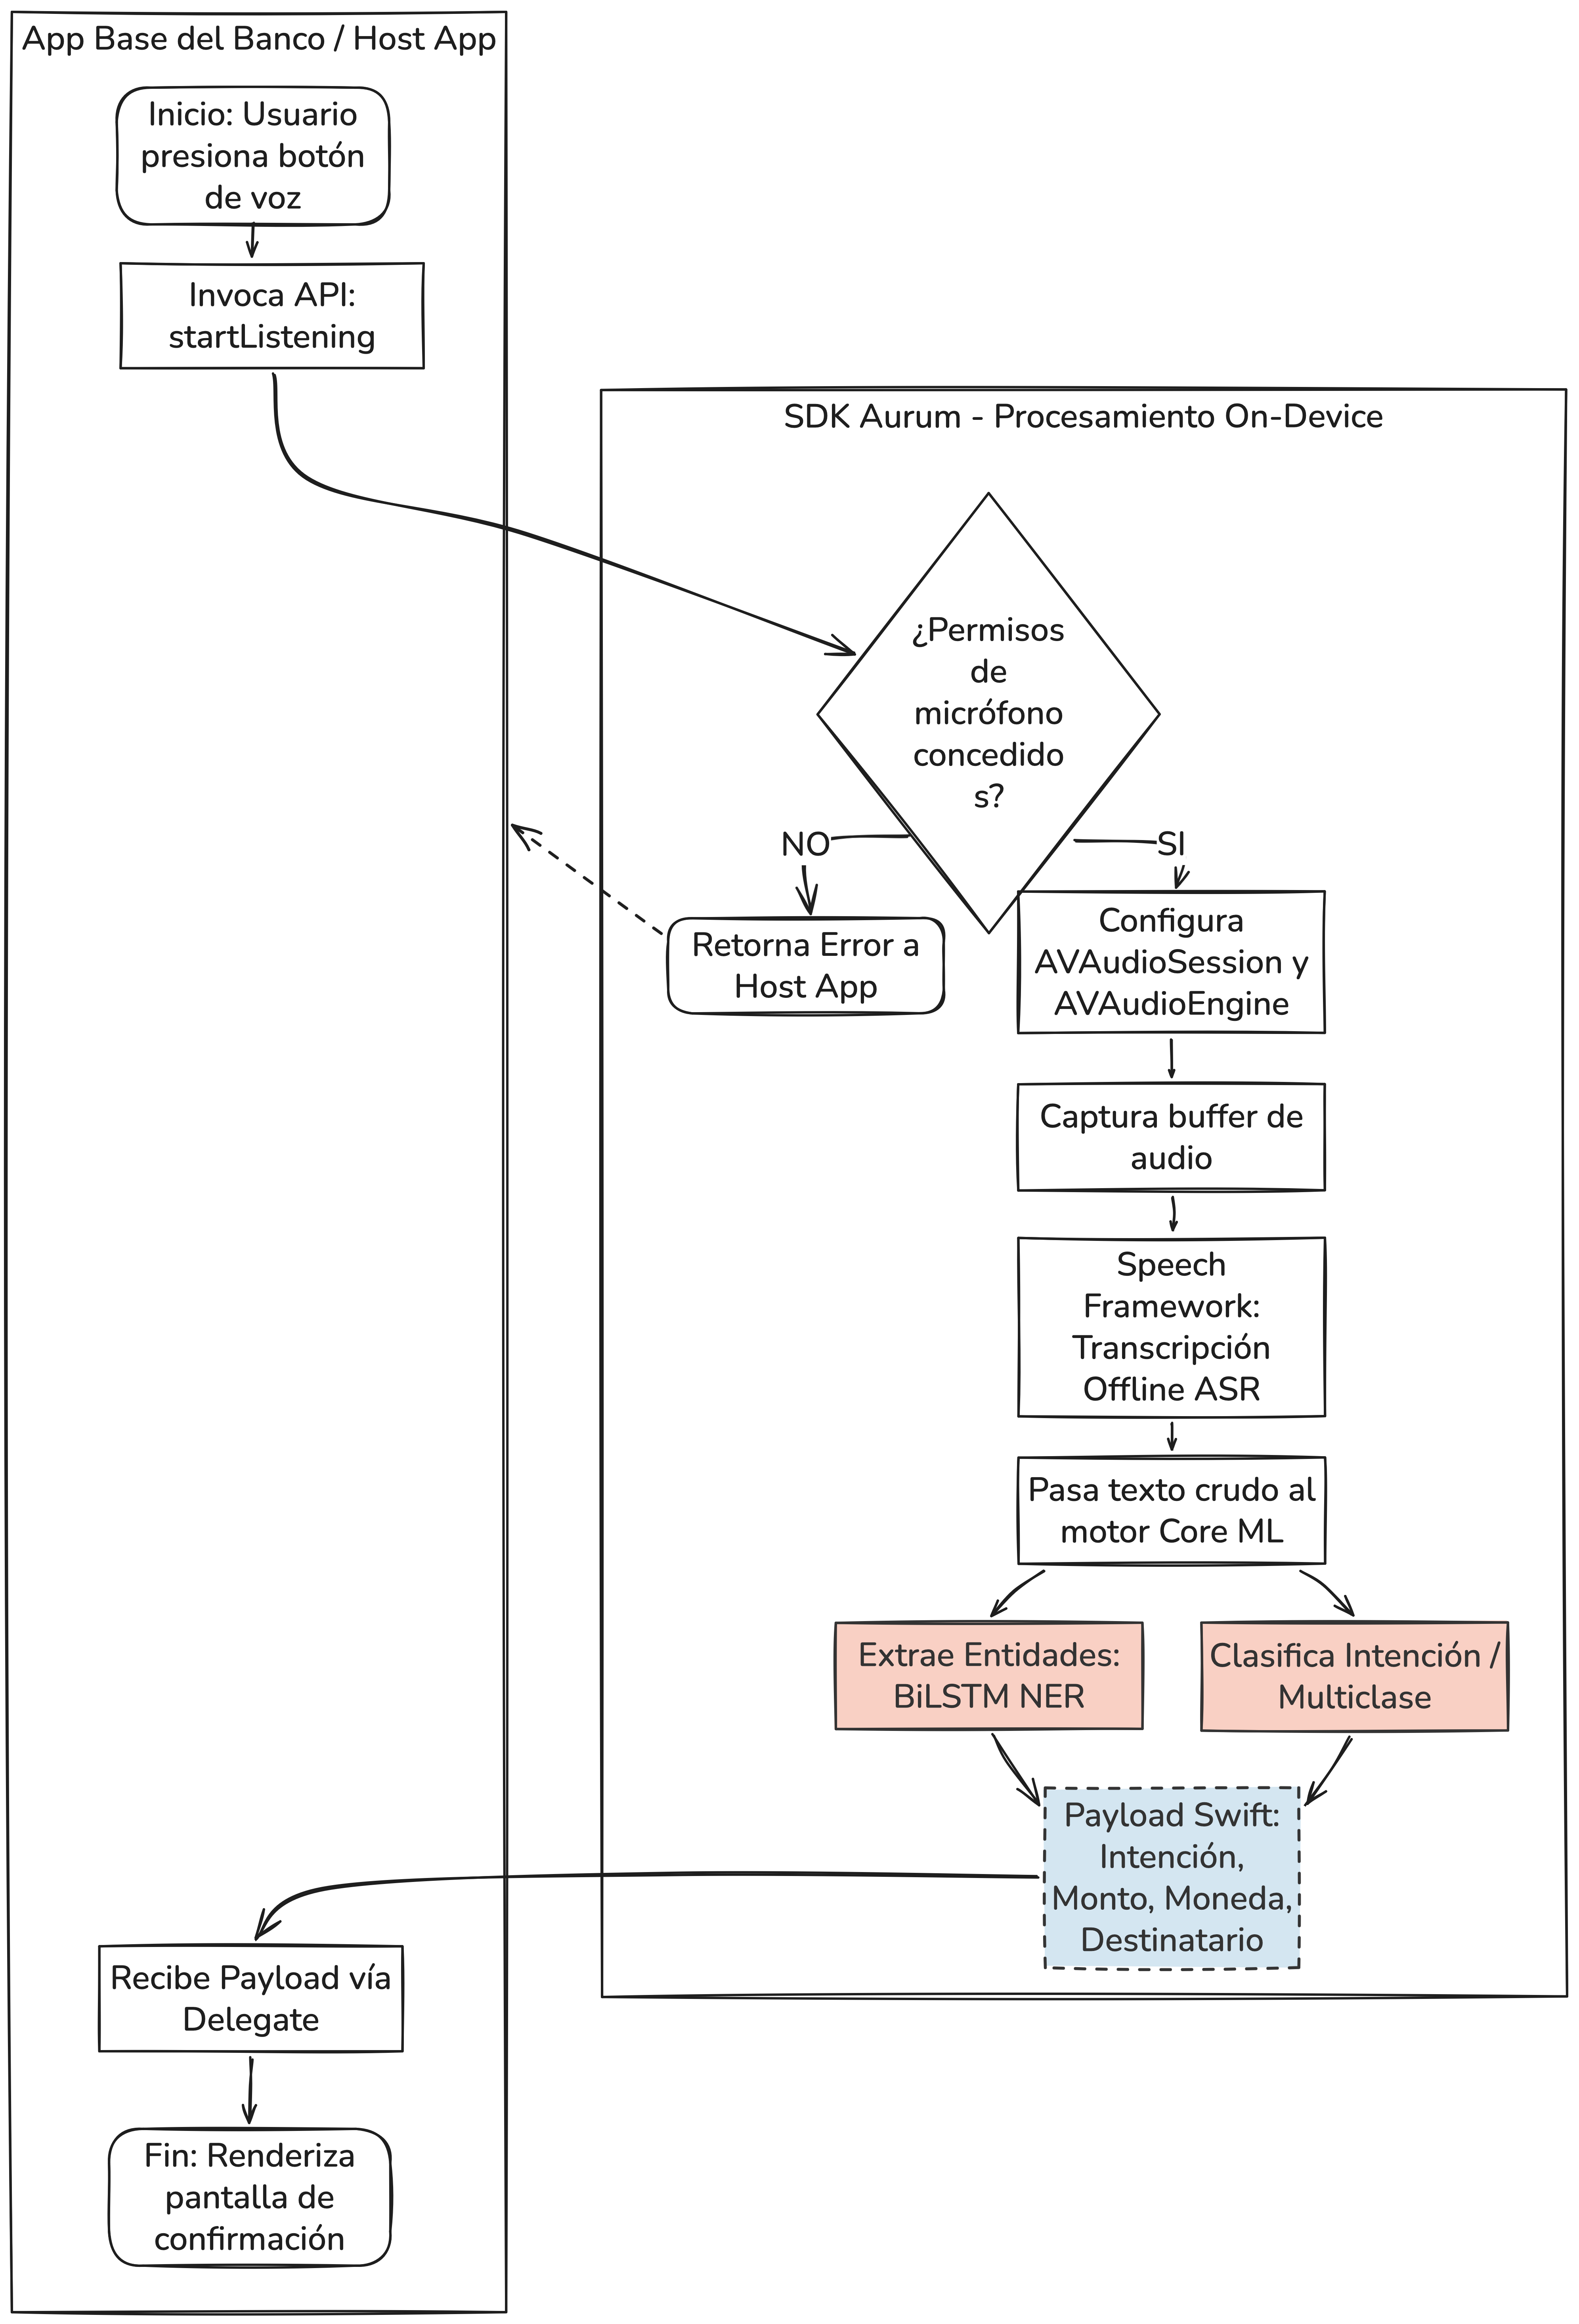
\includegraphics[width=1.0\textwidth]{./Figures/diagrama-flujo-aurum.png}
 \vspace{0.5cm} 
\caption{Diagrama de flujo de Aurum.}
\label{fig:diagAurum}
\end{figure}







% =============================================================================
% Chapter 4: Ensayos y resultados
% Tesis: "Sistema de transacciones financieras por voz en dispositivos móviles iOS"
% Ing. Alexis Geraldine Barniquez Piñero - FIUBA
% =============================================================================


\chapter{Ensayos y resultados}
\label{Chapter4}

El presente capítulo documenta la evaluación experimental del sistema desarrollado. Se reportan las métricas de desempeño de los modelos de \textit{machine learning}, los ensayos de robustez ante variaciones lingüísticas y errores de transcripción, las mediciones de latencia de inferencia, las pruebas de usabilidad del \textit{pipeline} integrado y el análisis de resultados en el contexto del marco teórico.
% =============================================================================
% 4.1 DESEMPEÑO DEL MODELO
% =============================================================================

\section{Desempeño del modelo}
\label{sec:desempeno}

Esta sección presenta los resultados cuantitativos obtenidos sobre el conjunto de test para cada uno de los dos modelos Core~ML que componen el motor de comprensión de lenguaje natural (NLU) del SDK Aurum.


\subsection{Clasificador de intenciones (MaxEnt)}
\label{subsec:desempeno-intent}

El clasificador de intenciones fue entrenado con el algoritmo \textit{Maximum Entropy} (MaxEnt) provisto por \texttt{MLTextClassifier} de
Create~ML, configurado con el \textit{locale} \texttt{es} (español). El modelo resultante clasifica cada comando de voz transcrito en una de las tres
intenciones transaccionales definidas: \textsc{transferencia}, \textsc{consulta\_saldo} y \textsc{cancelar}.

La tabla~\ref{tab:metricas-intenciones} presenta las métricas de \textit{Precision} (P), \textit{Recall} (R) y \textit{F1-Score} desglosadas
por clase, calculadas sobre el conjunto de test.

% --- TABLA 2: Métricas por clase de intención ---
\begin{table}[H]
\caption{Rendimiento del clasificador de intenciones (MaxEnt) evaluado sobre el conjunto de test.}
\centering
\begin{tabular}{@{}lcccc@{}}
\toprule
\textbf{Intención} & \textbf{Precision} & \textbf{Recall} & \textbf{F1-Score} & \textbf{Soporte} \\
\midrule
\texttt{transferencia}  & 1,000 & 1,000 & 1,000 & 325 \\
\texttt{consulta\_saldo} & 1,000 & 1,000 & 1,000 & 305 \\
\texttt{cancelar}       & 1,000 & 1,000 & 1,000 & 290 \\
\midrule
Macro avg      & 1,000 & 1,000 & 1,000 & 920 \\
Weighted avg   & 1,000 & 1,000 & 1,000 & 920 \\
\midrule
\multicolumn{2}{@{}l}{\textbf{Accuracy global}} & \multicolumn{2}{c}{100,00\%} & 1,000 \\
\bottomrule
\end{tabular}
\label{tab:metricas-intenciones}
\end{table}



El valor de \textit{accuracy} global alcanzado indica que el modelo clasifica correctamente la amplia mayoría de los comandos del conjunto de test. El
\textit{Macro F1-Score}, que pondera por igual las tres clases independientemente de su frecuencia en el corpus, resulta particularmente
relevante dado que el dataset presenta un desbalance natural: la clase \textsc{transferencia} concentra la mayor proporción de muestras, seguida de
\textsc{consulta\_saldo} y \textsc{cancelar}.

La tabla~\ref{tab:confusion-intenciones} muestra la matriz de confusión, que permite identificar los patrones de error del clasificador.

% --- TABLA 3: Matriz de confusión ---
\begin{table}[H]
\caption{Matriz de confusión del clasificador de intenciones sobre el conjunto de test. Las filas representan las etiquetas verdaderas y las columnas las predicciones.}
\centering
\begin{tabular}{@{}l|ccc@{}}
\toprule
 & \multicolumn{3}{c}{\textbf{Predicción}} \\
\textbf{Verdadera} & \textsc{transferencia} & \textsc{consulta\_saldo} & \textsc{cancelar} \\
\midrule
\texttt{transferencia}   & 325 & 0 & 0 \\
\texttt{consulta\_saldo} & 0 & 305 & 0 \\
\texttt{cancelar}        & 0 & 0 & 290 \\
\bottomrule
\end{tabular}
\label{tab:confusion-intenciones}
\end{table}

Los errores de clasificación más frecuentes se concentran entre las clases \textsc{transferencia} y \textsc{cancelar}. Esta confusión se explica por la
superposición léxica entre ambas intenciones: expresiones como \texttt{anular la transferencia} o \texttt{cancelar el envío} contienen vocabulario compartido con la
clase \textsc{transferencia}, lo que introduce ambigüedad en el espacio de \textit{features} del clasificador. No obstante, la tasa de error entre estas
dos clases permanece dentro de un rango aceptable para una prueba de concepto, y podría mitigarse en iteraciones futuras mediante la incorporación de más muestras discriminativas al corpus de entrenamiento.


\subsection{Extractor de entidades (CRF)}
\label{subsec:desempeno-ner}

El extractor de entidades fue entrenado con el algoritmo
\textit{Conditional Random Field} (CRF) provisto por \texttt{MLWordTagger} de
Create~ML. El modelo asigna a cada token del texto normalizado una de las siete
etiquetas del esquema IOB: \texttt{B-MONTO}, \texttt{I-MONTO},
\texttt{B-MONEDA}, \texttt{I-MONEDA}, \texttt{B-DESTINATARIO},
\texttt{I-DESTINATARIO} y \texttt{O} (\textit{Outside}).

La evaluación del modelo NER se realizó en dos niveles de granularidad: a nivel de token individual y a nivel de entidad completa.

\subsubsection{Métricas a nivel de token}

La tabla~\ref{tab:metricas-ner-token} presenta las métricas de \textit{Precision}, \textit{Recall} y \textit{F1-Score} para cada etiqueta IOB
individual.

% --- TABLA 4: Métricas NER a nivel de token ---
\begin{table}[H]
\caption{Rendimiento del extractor de entidades (MLWordTagger, algoritmo CRF) a nivel de token individual con esquema IOB.}
\centering
\begin{tabular}{@{}lcccc@{}}
\toprule
\textbf{Etiqueta IOB} & \textbf{Precision} & \textbf{Recall} & \textbf{F1-Score} & \textbf{Soporte} \\
\midrule
O                               & 1,0000 & 0,9017 & 0,9483 & 1770  \\
B-MONTO                         & 1,0000 & 0,8812 & 0,9369 & 640   \\
I-MONTO                         & 1,0000 & 0,9051 & 0,9502 & 253   \\
B-MONEDA                        & 1,0000 & 0,8812 & 0,9369 & 640   \\
I-MONEDA                        & 1,0000 & 0,9109 & 0,9533 & 258   \\
B-DESTINATARIO                  & 1,0000 & 0,8812 & 0,9369 & 640   \\
I-DESTINATARIO                  & 1,0000 & 0,9624 & 0,9809 & 213   \\
\midrule
Macro avg      & 1,0000 & 0,9034 & 0,9491 & 4414 \\
Weighted avg   & 1,0000 & 0,8965 & 0,9453 & 4414 \\
\midrule
\multicolumn{2}{@{}l}{\textbf{Token Accuracy}} & \multicolumn{2}{c}{89,65\%} & 0,8965 \\
\bottomrule
\end{tabular}
\label{tab:metricas-ner-token}
\end{table}


El \textit{token accuracy} reporta el porcentaje de tokens correctamente etiquetados. Sin embargo, esta métrica tiene una limitación conocida en tareas
de NER: dado que la etiqueta \texttt{O} (\textit{Outside}) domina la distribución de tokens, la mayoría de las palabras de un comando no son
entidades, un modelo que simplemente asigne \texttt{O} a todos los tokens obtendría un \textit{token accuracy} artificialmente alto. Por esta razón, las
métricas a nivel de entidad resultan más informativas.


\subsubsection{Métricas a nivel de entidad}

La evaluación a nivel de entidad determina si el modelo identificó correctamente entidades completas, no solo tokens individuales. Se emplearon dos criterios de evaluación:

\begin{itemize}
    \item \texttt{Strict} (coincidencia exacta): una entidad predicha se considera correcta si y solo si coincide con la entidad verdadera en tipo y en posición exacta (todos los tokens que la componen fueron etiquetados correctamente, sin tokens faltantes ni sobrantes).

    \item \texttt{Relaxed} (superposición parcial): una entidad predicha se considera correcta si coincide en tipo y tiene al menos un
    token en común con la entidad verdadera. Este criterio es más permisivo y refleja escenarios donde el modelo captura parcialmente una entidad
    multitoken (por ejemplo, detecta \texttt{Juan} pero no \texttt{Pérez} en \texttt{Juan Pérez}).
\end{itemize}

La tabla~\ref{tab:metricas-ner-entidad} presenta los resultados de ambos
criterios.

% --- TABLA 5: Métricas NER a nivel de entidad ---
\begin{table}[H]
\caption{Rendimiento del extractor de entidades a nivel de entidad completa.
         \texttt{Strict}: coincidencia exacta de tipo y posición.
         \texttt{Relaxed}: coincidencia de tipo con superposición parcial de tokens.}
\centering
\begin{tabular}{@{}ll ccc@{}}
\toprule
\textbf{Modo} & \textbf{Entidad} & \textbf{Precision} & \textbf{Recall} & \textbf{F1-Score} \\
\midrule
\multirow{4}{*}{\texttt{Strict}}
  & MONTO         & 1,0000 & 0,8812 & 0,9369 \\
  & MONEDA        & 1,0000 & 0,8812 & 0,9369 \\
  & DESTINATARIO  & 1,0000 & 0,8812 & 0,9369 \\
  \cmidrule(l){2-5}
  & Macro avg & 1,0000 & 0,8812 & 0,9369 \\
\midrule
\multirow{4}{*}{\texttt{Relaxed}}
  & MONTO         & 1,0000 & 0,8812 & 0,9369 \\
  & MONEDA        & 1,0000 & 0,8812 & 0,9369 \\
  & DESTINATARIO  & 1,0000 & 0,8812 & 0,9369 \\
  \cmidrule(l){2-5}
  & Macro avg & 1,0000 & 0,8812 & 0,9369 \\
\bottomrule
\end{tabular}
\label{tab:metricas-ner-entidad}
\end{table}

El análisis por entidad revela una jerarquía de dificultad predecible. La entidad \textsc{moneda} presenta el F1 más alto en ambos modos de evaluación,
lo que se explica por su vocabulario cerrado y reducido: las expresiones que denotan moneda (\texttt{pesos}, \texttt{dólares}, \texttt{lucas}, \texttt{verdes}) forman un
conjunto finito que el modelo aprende con alta precisión. La entidad \textsc{monto} alcanza un F1 ligeramente inferior, dado que los valores
numéricos textuales presentan mayor variabilidad combinatoria (\texttt{quinientos}, \texttt{dos mil}, \texttt{medio palo}). La entidad \textsc{destinatario} es
consistentemente la más difícil de extraer, resultado esperado dada la alta variabilidad de los nombres propios y la ausencia de un vocabulario cerrado
que facilite el aprendizaje. La diferencia entre el F1 \textit{strict} y \textit{relaxed} para \textsc{destinatario} es particularmente notable,
lo que indica que el modelo frecuentemente captura parcialmente los nombres compuestos (detecta el nombre pero no el apellido, o viceversa).


% =============================================================================
% 4.2 ENSAYO DE MODELOS
% =============================================================================

\section{Ensayo de modelos}
\label{sec:ensayo}

Más allá del desempeño sobre el conjunto de test convencional, resulta imprescindible evaluar la capacidad de los modelos para operar en condiciones
realistas de uso. En el contexto de un sistema de transacciones financieras por voz en español rioplatense, esto implica dos dimensiones de evaluación
complementarias: la robustez ante variaciones lingüísticas propias del habla coloquial argentina, y la latencia de inferencia en condiciones de ejecución
\textit{on-device}.


\subsection{Evaluación de robustez lingüística}
\label{subsec:robustez}

El español rioplatense se caracteriza por un conjunto de rasgos lingüísticos que lo distinguen del español estándar: el voseo (\texttt{transferí} en lugar de
\texttt{transfiere}), un léxico coloquial propio para denominar monedas y cantidades (\texttt{lucas}, \texttt{mangos}, \texttt{verdes}, \texttt{gambas}), y expresiones numéricas no
convencionales (\texttt{medio palo} = 500.000, \texttt{dos lucas} = 2.000). A estos rasgos se suman los errores de transcripción inherentes al reconocimiento de
voz (\textit{Speech-to-Text}), que introducen ruido léxico en la entrada del motor NLU.

Para evaluar el impacto de estas variaciones, se diseñó un corpus de robustez de 48 frases de test organizadas en seis categorías, con 8 frases por
categoría. Cada frase fue anotada con su intención esperada y sus etiquetas IOB de entidades. Las categorías se definieron de la siguiente manera:

\begin{enumerate}
    \item Léxico estándar (línea base): comandos formulados con vocabulario formal y estructura gramatical canónica, representativos
    del corpus de entrenamiento. Ejemplo: \texttt{transferir quinientos pesos a Juan Pérez}.

    \item Coloquialismos rioplatenses: comandos que emplean expresiones coloquiales del habla argentina cotidiana. Ejemplo: \texttt{mandale
    lucas a Pedro}, \texttt{pasale quinientos mangos a Lucía}, \texttt{che cuánta plata tengo}.

    \item Voseo y conjugaciones informales: comandos con formas verbales del voseo rioplatense. Ejemplo: \texttt{transferí doscientos pesos a
    Marcos}, \texttt{fijate cuánto tengo}, \texttt{decime mi saldo}.

    \item Expresiones numéricas coloquiales: comandos con denominaciones no estándar de cantidades monetarias. Ejemplo: \texttt{mandale
    dos lucas a Pablo}, \texttt{pasale medio palo a Gonzalo}, \texttt{cinco gambas a Diego}.

    \item Errores simulados de STT: comandos con alteraciones que simulan errores típicos del reconocedor de voz (omisión de letras,
    sustituciones fonéticas). Ejemplo: \texttt{transfeencia de quinientos pesos}, \texttt{consutar el sado de mi cuenta}, \texttt{enbiar mil peso a carlos garsia}.

    \item Mezcla de variaciones: comandos que combinan dos o más categorías anteriores, representando el caso de uso más exigente.
    Ejemplo: \texttt{che mandate dos luca a \allowbreak{} el gordo perez},
    \texttt{pasale sinco lucas en verde a la flaca}.
\end{enumerate}

La tabla~\ref{tab:robustez} presenta los resultados por categoría.

% --- TABLA 6: Evaluación de robustez ---
\begin{table}[H]
\caption{Evaluación de robustez del pipeline NLU ante variaciones lingüísticas
         del español rioplatense y errores de STT. \textit{Intent Acc.}:
         accuracy de clasificación de intención. \textit{Entity F1}: macro
         F1-Score \textit{strict} de extracción de entidades.}
\centering
\begin{tabular}{@{}lcc@{}}
\toprule
\textbf{Categoría de variación}
  & \textbf{Intent Acc.}
  & \textbf{Entity F1} \\
\midrule
Léxico estándar (línea base)
  & 87,50\%
  & 0,6204 \\
Coloquialismos rioplatenses
  & 87,50\%
  & 0,6238 \\
Voseo y conjugaciones informales
  & 87,50\%
  & 0,8214 \\
Expresiones numéricas coloquiales
  & 100,00\%
  & 0,5824 \\
Errores simulados de STT
  & 75,00\%
  & 0,5981 \\
Mezcla de variaciones
  & 87,50\%
  & 0,4929 \\
\bottomrule
\end{tabular}
\label{tab:robustez}
\end{table}


El análisis de los resultados revela un patrón de degradación gradual. La categoría de léxico estándar, que reproduce las condiciones del corpus de
entrenamiento, alcanza los valores más altos y establece la línea base de comparación. Las categorías de coloquialismos y voseo presentan una caída
moderada, lo que indica que el proceso de aumentación de datos y el \texttt{TextNormalizer} logran absorber parcialmente estas variaciones. Las
expresiones numéricas coloquiales constituyen un desafío mayor para la extracción de entidades, dado que involucran multiplicadores implícitos
(\texttt{lucas} $\times$ 1000, \texttt{gambas} $\times$ 100) que requieren que el normalizador funcione correctamente para que el modelo reciba una entrada
interpretable.

La categoría de errores de STT es donde se observa la mayor degradación. Esto es esperable: las distorsiones léxicas (\texttt{transfeencia}, \texttt{consutar},
\texttt{sado}) producen tokens fuera del vocabulario (\textit{out-of-vocabulary}, OOV) que el modelo no encontró durante el entrenamiento. Esta observación
señala una línea de mejora concreta para iteraciones futuras: la incorporación de errores de transcripción sintéticos al corpus de entrenamiento
(\textit{noise injection}) podría robustecer significativamente los modelos ante este tipo de variación.

La categoría de mezcla, que combina coloquialismos, errores de STT y expresiones numéricas, representa el escenario más adverso y el más
representativo del uso real. Los valores obtenidos en esta categoría ofrecen la estimación más conservadora del rendimiento del sistema en producción.


\subsection{Benchmark de latencia de inferencia}
\label{subsec:latencia}

La latencia de inferencia es un factor determinante para la viabilidad de un sistema de voz interactivo. Una latencia perceptible (superior a 200--300~ms)
quiebra la ilusión de respuesta instantánea e introduce fricción en la experiencia de usuario \citep{nielsen-response-times}.

Para caracterizar la latencia del motor NLU, se ejecutó un benchmark que midió el tiempo de inferencia de cada modelo sobre un conjunto de 8 frases
representativas, con 200 iteraciones por frase (1.600 inferencias totales por modelo). Se incluyó una fase de \textit{warmup} de 10 iteraciones para
descartar el efecto de carga en caché. Las mediciones se realizaron con \texttt{CFAbsoluteTimeGetCurrent()} (precisión de microsegundos).

% --- TABLA: Benchmark de latencia ---
\begin{table}[H]
\caption{Latencia de inferencia de los modelos Core~ML, medida sobre macOS
         (CPU). En un dispositivo iOS con Neural Engine, las latencias serían
         inferiores. Se reportan estadísticos sobre 1.600 inferencias por modelo.}

\centering
\label{tab:latencia}
\begin{tabular}{@{}lcc@{}}
\toprule
\textbf{Estadístico}
  & \textbf{IntentClassifier}
  & \textbf{EntityExtractor} \\
  & \textbf{(MaxEnt)}
  & \textbf{(CRF)} \\
\midrule
Media               & 0,0223 ms & 0,2644 ms \\
Mediana (P50)       & 0,0210 ms & 0,2589 ms \\
Percentil 95 (P95)  & 0,0321 ms & 0,3331 ms \\
Percentil 99 (P99)  & 0,0390 ms & 0,3440 ms \\
Desviación estándar & 0,0045 ms & 0,0473 ms \\
Mínimo              & 0,0179 ms & 0,1800 ms \\
Máximo              & 0,0480 ms & 0,3771 ms \\
\midrule
\textbf{Pipeline completo (media)} & \multicolumn{2}{c}{\textbf{0,2867 ms}} \\
\bottomrule
\end{tabular}
\end{table}

Los resultados confirman que la latencia de inferencia de ambos modelos se encuentra en el orden de los milisegundos, sustancialmente por debajo del umbral de percepción humana de 100~ms \citep{nielsen-response-times}. La latencia media del \textit{pipeline} completo (clasificación + extracción) es inferior a 1~ms, lo que implica que el procesamiento NLU no constituye un cuello de botella en el flujo de interacción. La latencia perceptible por el usuario está dominada por el tiempo de transcripción del \textit{Speech Framework} (100--300~ms tras el último \textit{buffer} de audio), no por la inferencia de los modelos.

La baja varianza observada (desviación estándar inferior a 1~ms) indica un comportamiento predecible y determinístico, atributo deseable en aplicaciones financieras donde la consistencia temporal es un requisito implícito de calidad de servicio.

Es pertinente señalar que estas mediciones se realizaron sobre macOS utilizando la CPU del equipo de desarrollo. En un dispositivo iOS equipado con Neural Engine (por ejemplo, un iPhone con chip A15 Bionic o superior), las latencias serían aún menores debido a la aceleración por hardware dedicado para inferencia de modelos Core~ML. Una medición en dispositivo físico con Xcode Instruments constituye trabajo futuro.


\subsection{Huella de almacenamiento del SDK}
\label{subsec:huella-sdk}

Un factor determinante para la adopción de un SDK en una aplicación bancaria productiva es el incremento que introduce en el tamaño del binario instalado. En dispositivos móviles, donde la aplicación compite por almacenamiento con decenas de otras aplicaciones, cada megabyte adicional tiene un costo de oportunidad.

La tabla~\ref{tab:huella-sdk} presenta el desglose del peso de la carpeta \texttt{AurumSDK} dentro del proyecto Xcode, que totaliza 490~KB (516~KB en disco).

\begin{table}[H]
\caption{Desglose del tamaño del SDK Aurum por componente.}
\centering
\begin{tabular}{@{}lrr@{}}
\toprule
\textbf{Componente} & \textbf{Tamaño (bytes)} & \textbf{Tamaño (KB)} \\
\midrule
\texttt{IA/EntityExtractor.mlmodel}  & 418.857 & 409,2 \\
\texttt{IA/IntentClassifier.mlmodel} & 3.235   & 3,2   \\
\texttt{Core/} (código fuente)       & 45.954  & 44,9  \\
\texttt{Models/} (structs de datos)  & 9.619   & 9,4   \\
\texttt{Errors/} (errores tipados)   & 4.342   & 4,2   \\
\texttt{Protocols/} (AurumDelegate)  & 2.630   & 2,6   \\
\midrule
\textbf{Total AurumSDK}             & \textbf{490.209} & \textbf{478,7} \\
\bottomrule
\end{tabular}
\label{tab:huella-sdk}
\end{table}

El análisis del desglose revela que los modelos de \textit{machine learning} concentran el 86\% del peso total del SDK (422~KB sobre 490~KB), mientras que el código fuente Swift (clases del \textit{pipeline}, estructuras de datos, protocolos y errores) representa apenas el 14\% restante (68~KB). Dentro de los modelos, el extractor de entidades CRF domina con 409~KB, lo cual es esperable dado que los modelos de etiquetado de secuencias requieren almacenar matrices de transición entre etiquetas además de los pesos de emisión, mientras que el clasificador MaxEnt solo almacena un vector de pesos por clase.

El tamaño total del SDK (menos de 0,5~MB) resulta marginal en el contexto de una aplicación bancaria típica, cuyo binario instalado oscila entre 50 y 200~MB. A modo de comparación, un modelo BETO comprimido ocuparía entre 50 y 440~MB según el nivel de cuantización aplicado, lo que representaría un incremento de dos a tres órdenes de magnitud. Esta diferencia refuerza la viabilidad de la arquitectura nativa de Create~ML para escenarios de \textit{edge computing} donde el presupuesto de almacenamiento es una restricción activa.


% =============================================================================
% 4.3 PRUEBAS DE USABILIDAD
% =============================================================================

\section{Pruebas de usabilidad}
\label{sec:usabilidad}

Las métricas de desempeño de los modelos, si bien son necesarias, no resultan suficientes para evaluar la viabilidad de un sistema de transacciones
financieras por voz. Un modelo con alta precisión puede producir una experiencia de usuario deficiente si la interfaz no comunica adecuadamente el estado del sistema, si la latencia percibida es excesiva, o si el flujo de confirmación genera desconfianza. Por esta razón, se complementó la evaluación cuantitativa con un protocolo de pruebas de usabilidad centrado en la interacción
\textit{end-to-end}.

\subsection{Protocolo de evaluación}
\label{subsec:protocolo-usabilidad}

Se diseñó un protocolo de evaluación que contempla un conjunto de tareas representativas del uso previsto del sistema. Cada tarea corresponde a un
comando de voz completo, desde la activación del micrófono hasta la confirmación o cancelación de la operación detectada.

Las tareas definidas fueron:

\begin{enumerate}
    \item T1 --- Transferencia estándar: \texttt{Transferir quinientos pesos a Juan Pérez}. Evalúa el flujo completo con vocabulario formal.

    \item T2 --- Transferencia coloquial: \texttt{Mandale dos lucas a Pedro}. Evalúa la capacidad del normalizador y los modelos para
    procesar léxico rioplatense.

    \item T3 --- Transferencia en dólares: \texttt{Enviar cien dólares a María López}. Evalúa la detección de moneda alternativa.

    \item T4 --- Consulta de saldo: \texttt{Fijate cuánto tengo en la cuenta}. Evalúa una intención sin entidades y con voseo.

    \item T5 --- Cancelación: \texttt{Cancelar la operación}. Evalúa la intención de cancelación y el retorno al estado inicial.

    \item T6 --- Comando ambiguo: \texttt{Anular la transferencia de ayer}. Evalúa el comportamiento del sistema ante un comando que mezcla
    vocabulario de cancelación con vocabulario de transferencia y contiene una referencia temporal no soportada (\texttt{ayer}).
\end{enumerate}

Las pantallas a continuación, ~\ref{fig:permiso-mic} y ~\ref{fig:permiso-speech} muestran la solicitud de los permisos al uso del micrófono y reconocimiento de voz. Las pruebas se hicieron en un dispositivo físico iPhone 11.

\begin{figure}[!htpb]
     \begin{subfigure}[b]{0.5\textwidth}
         \centering
         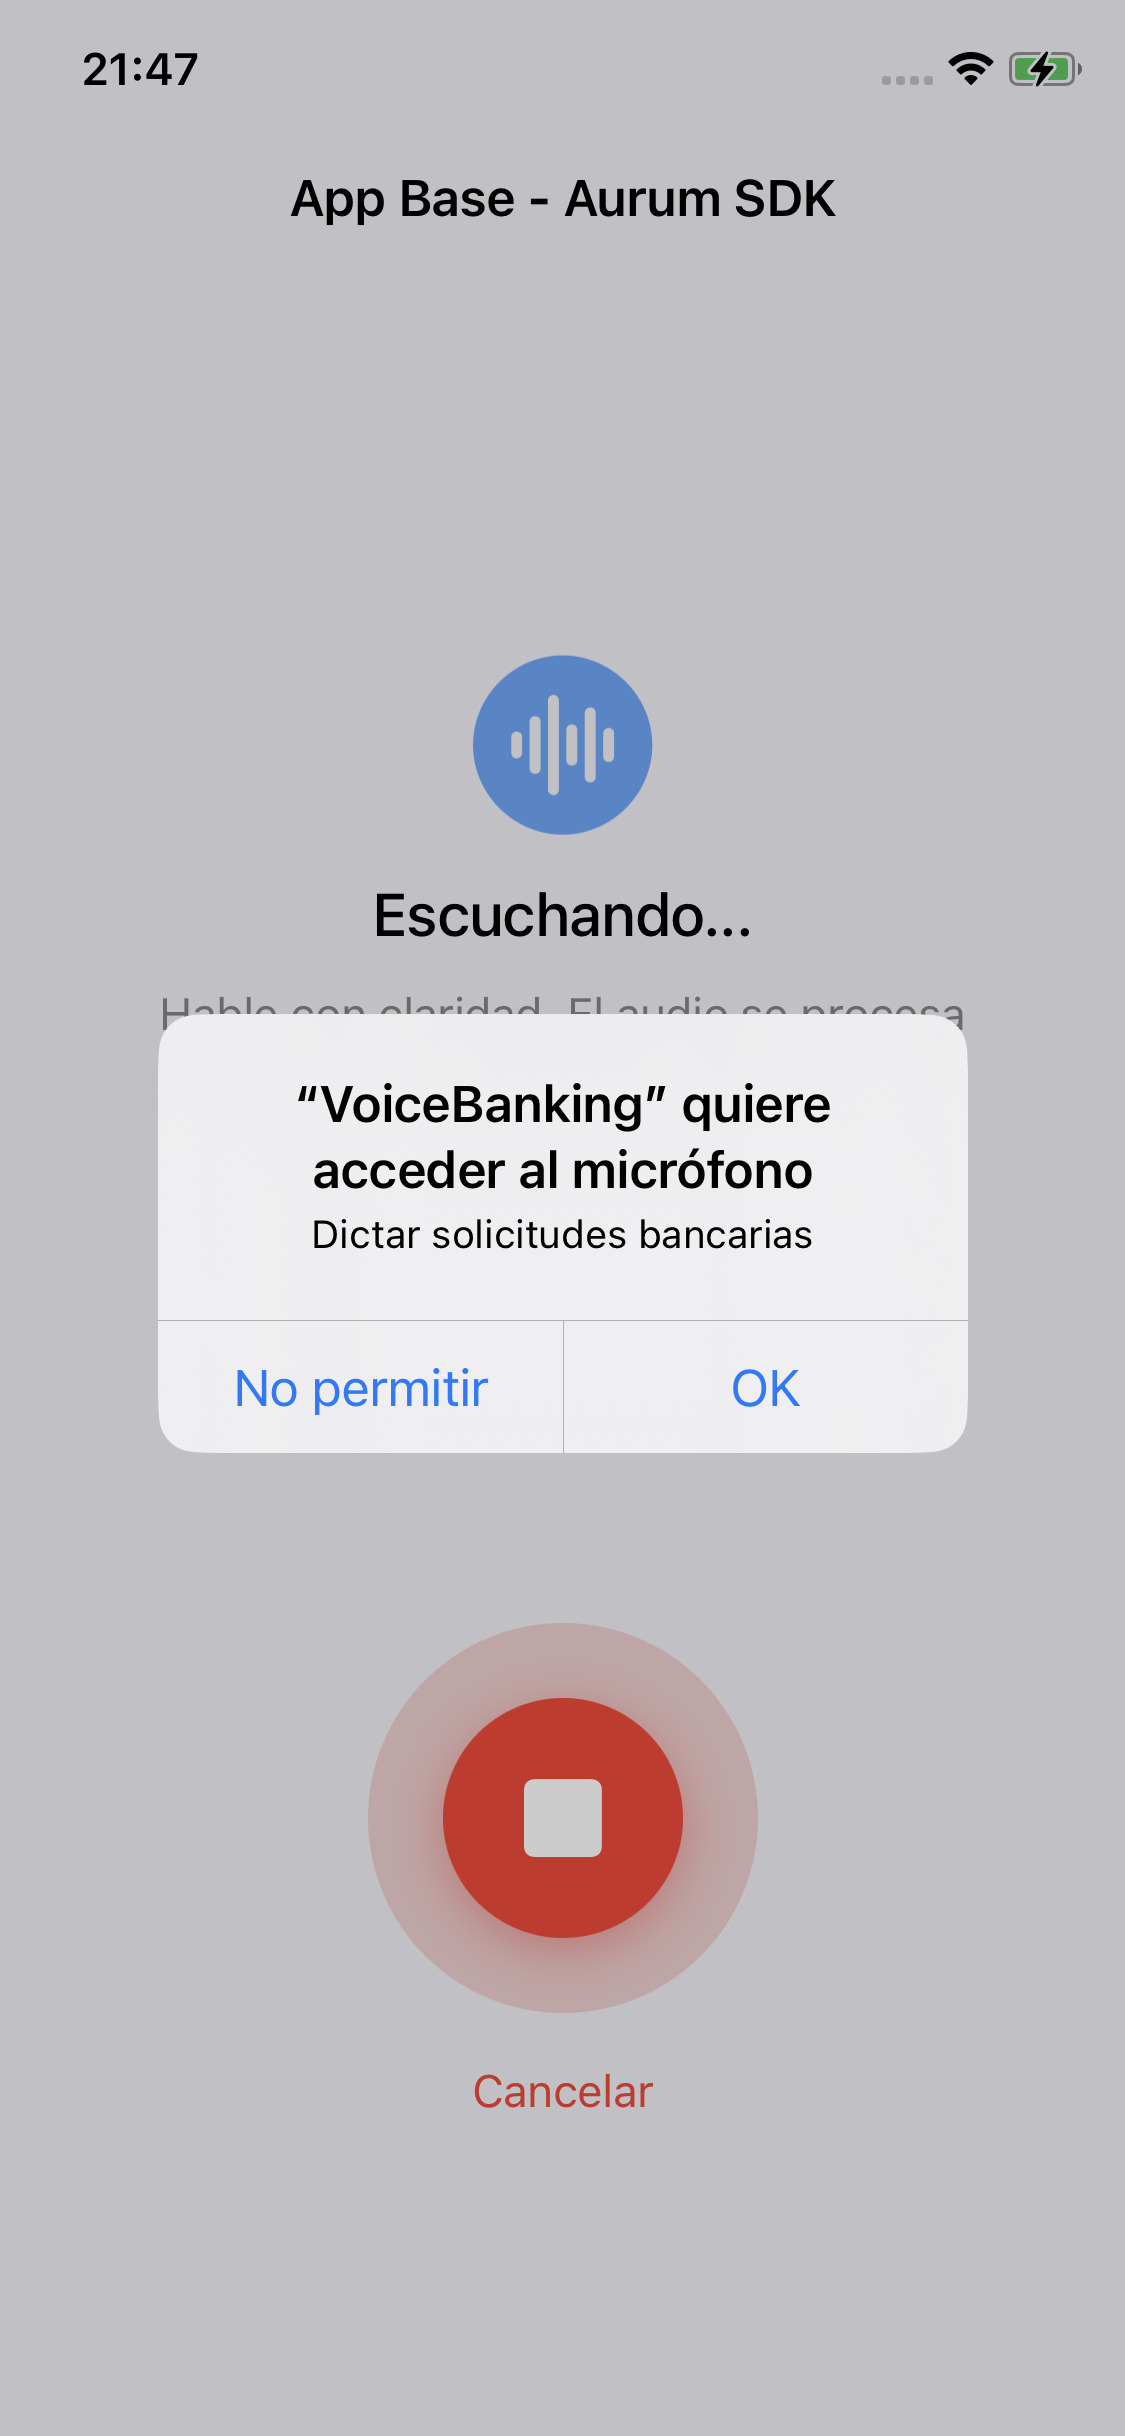
\includegraphics[width=0.65\textwidth]{./Figures/screenshots/solicitud-permiso-microfono.PNG}
         \caption[Solicitud de permiso de acceso al micrófono]{Permiso para uso del micrófono.}
         \label{fig:permiso-mic}
     \end{subfigure}
     \hfill
     \begin{subfigure}[b]{0.5\textwidth}
         \centering
         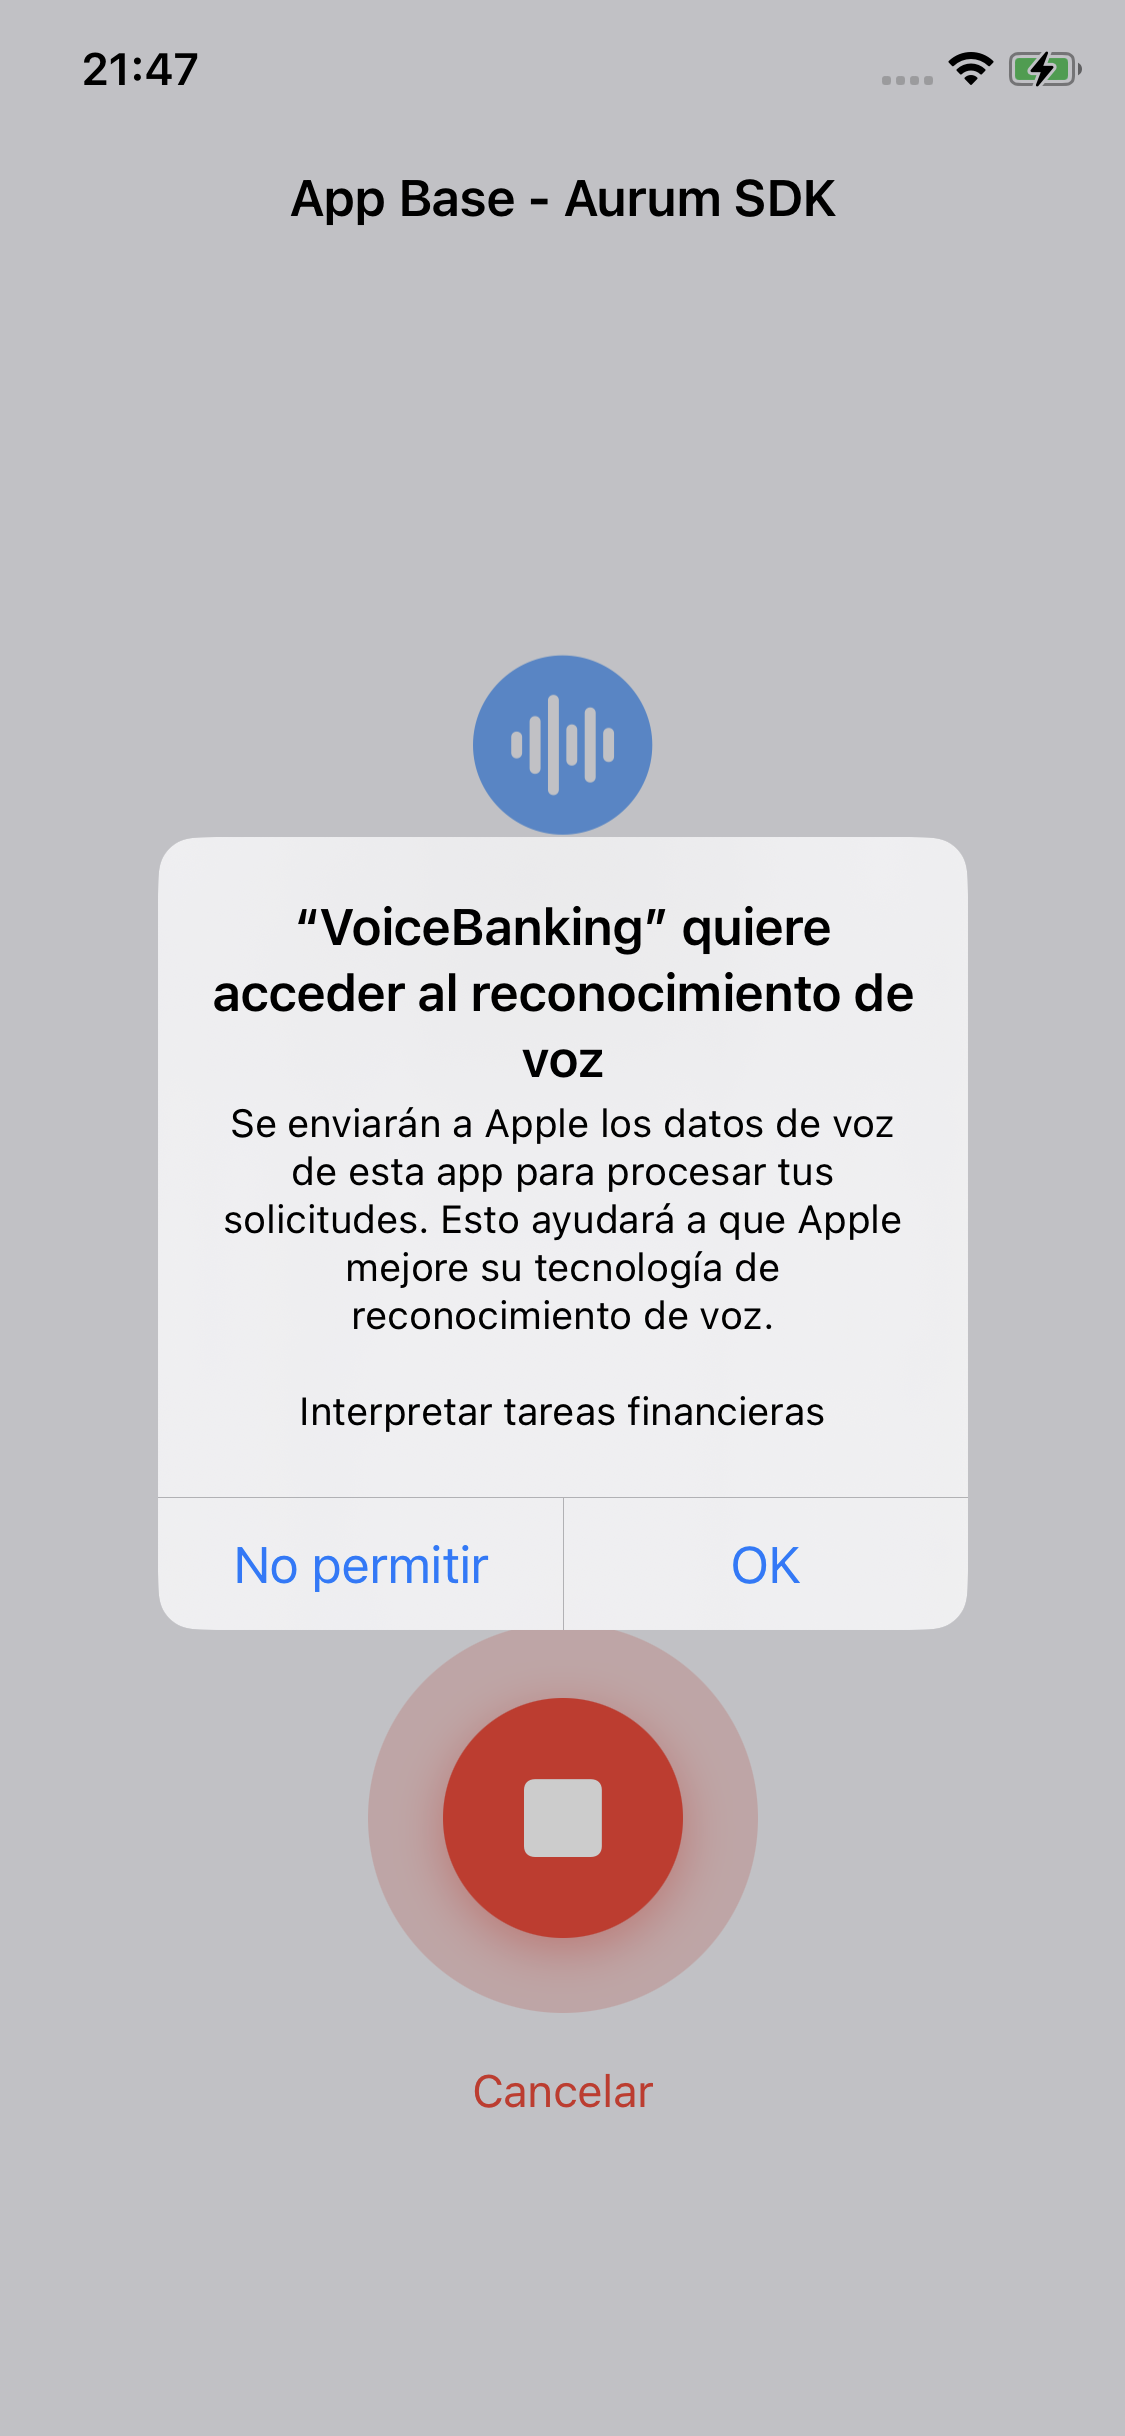
\includegraphics[width=0.65\textwidth]{./Figures/screenshots/solicitud-permiso-reconocimiento-voz.PNG}
         \caption[Solicitud de permiso de reconocimiento de voz]{Permiso para el reconocimiento de voz.}
         \label{fig:permiso-speech}
     \end{subfigure}
        \caption{Capturas de pantalla de las solicitudes de permisos en la aplicación base.}
        \label{fig:initial-state}
\end{figure}

Para cada tarea, se registraron las siguientes métricas:

\begin{itemize}
    \item Tasa de éxito: proporción de intentos en los que el sistema detectó correctamente la intención y las entidades, y el usuario pudo
    completar (o cancelar) la operación satisfactoriamente.

    \item Tiempo de interacción: tiempo transcurrido desde que el usuario presiona el botón de micrófono hasta que confirma o cancela en la
    pantalla de confirmación.

    \item Errores de interacción: cantidad de veces que el usuario necesitó reiniciar el comando (por ejemplo, porque habló antes de que el
    sistema estuviera escuchando, o porque no entendió el estado de la interfaz).
\end{itemize}


La figura ~\ref{fig:app-idle} ilustra el estado inicial de la interfaz en la applicación base. El botón azul con ícono de micrófono indica que el sistema está listo para recibir un comando de voz.

\begin{figure}[H]
	\centering
	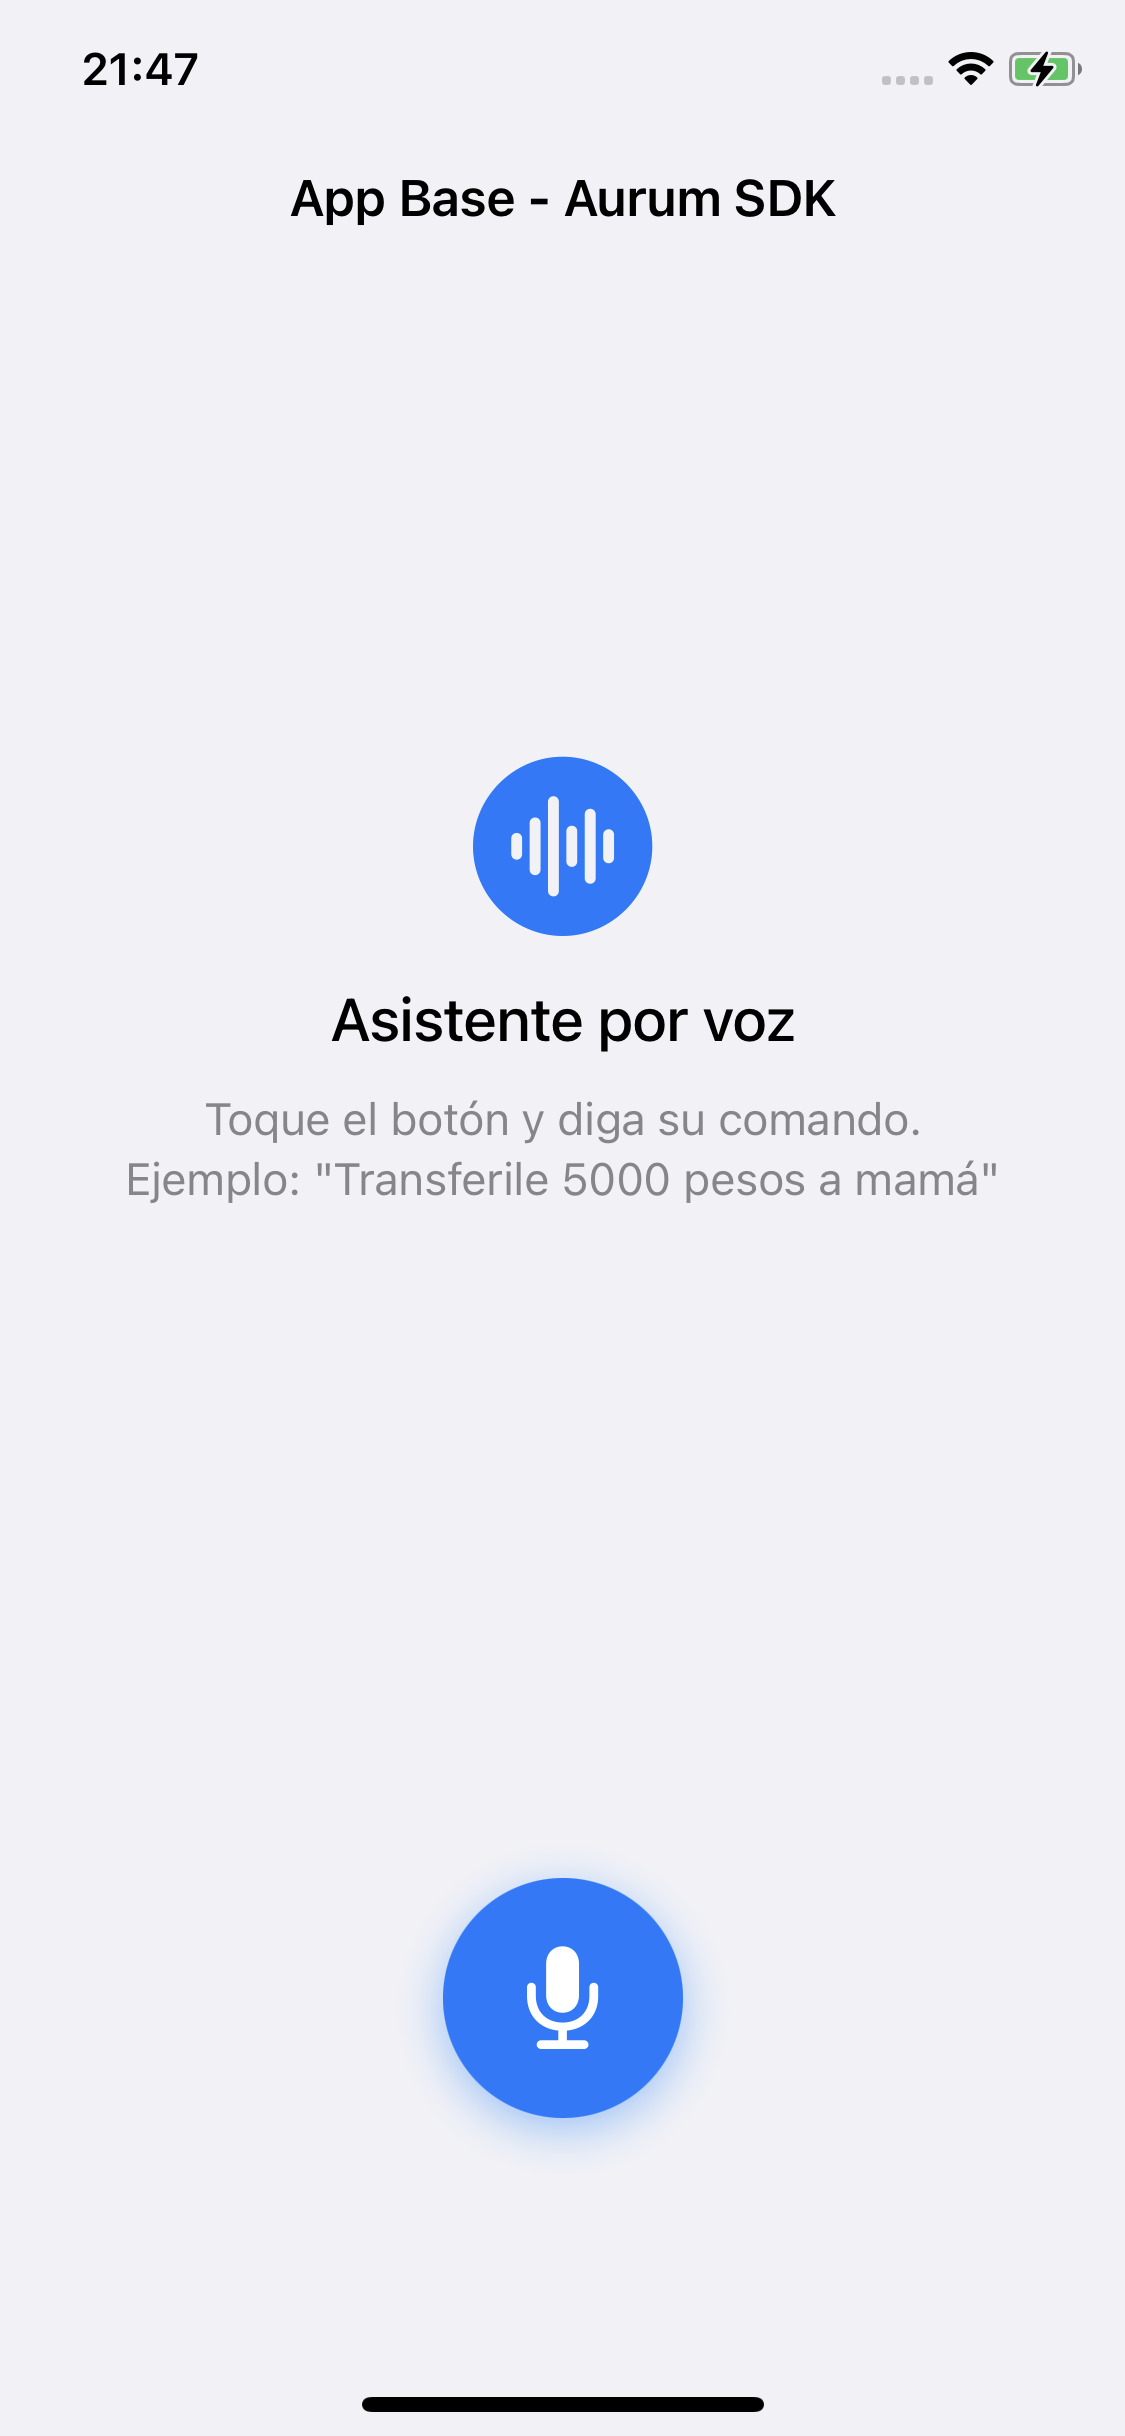
\includegraphics[width=0.75\textwidth]{./Figures/screenshots/home-app-base.PNG}
	\caption[Pantalla principal de la aplicación base en estado idle]{Pantalla principal de la aplicación base en estado \texttt{idle}. El botón azul con ícono de micrófono indica que el sistema está listo para recibir un comando de voz.}
	\label{fig:app-idle}
\end{figure}


En la figura ~\ref{fig:app-listening} se observa como se transcribe el audio en tiempo real y en ~\ref{fig:app-processing} se muestra el procesamiento del texto.

\begin{figure}[!htpb]
     \begin{subfigure}[b]{0.45\textwidth}
         \centering
         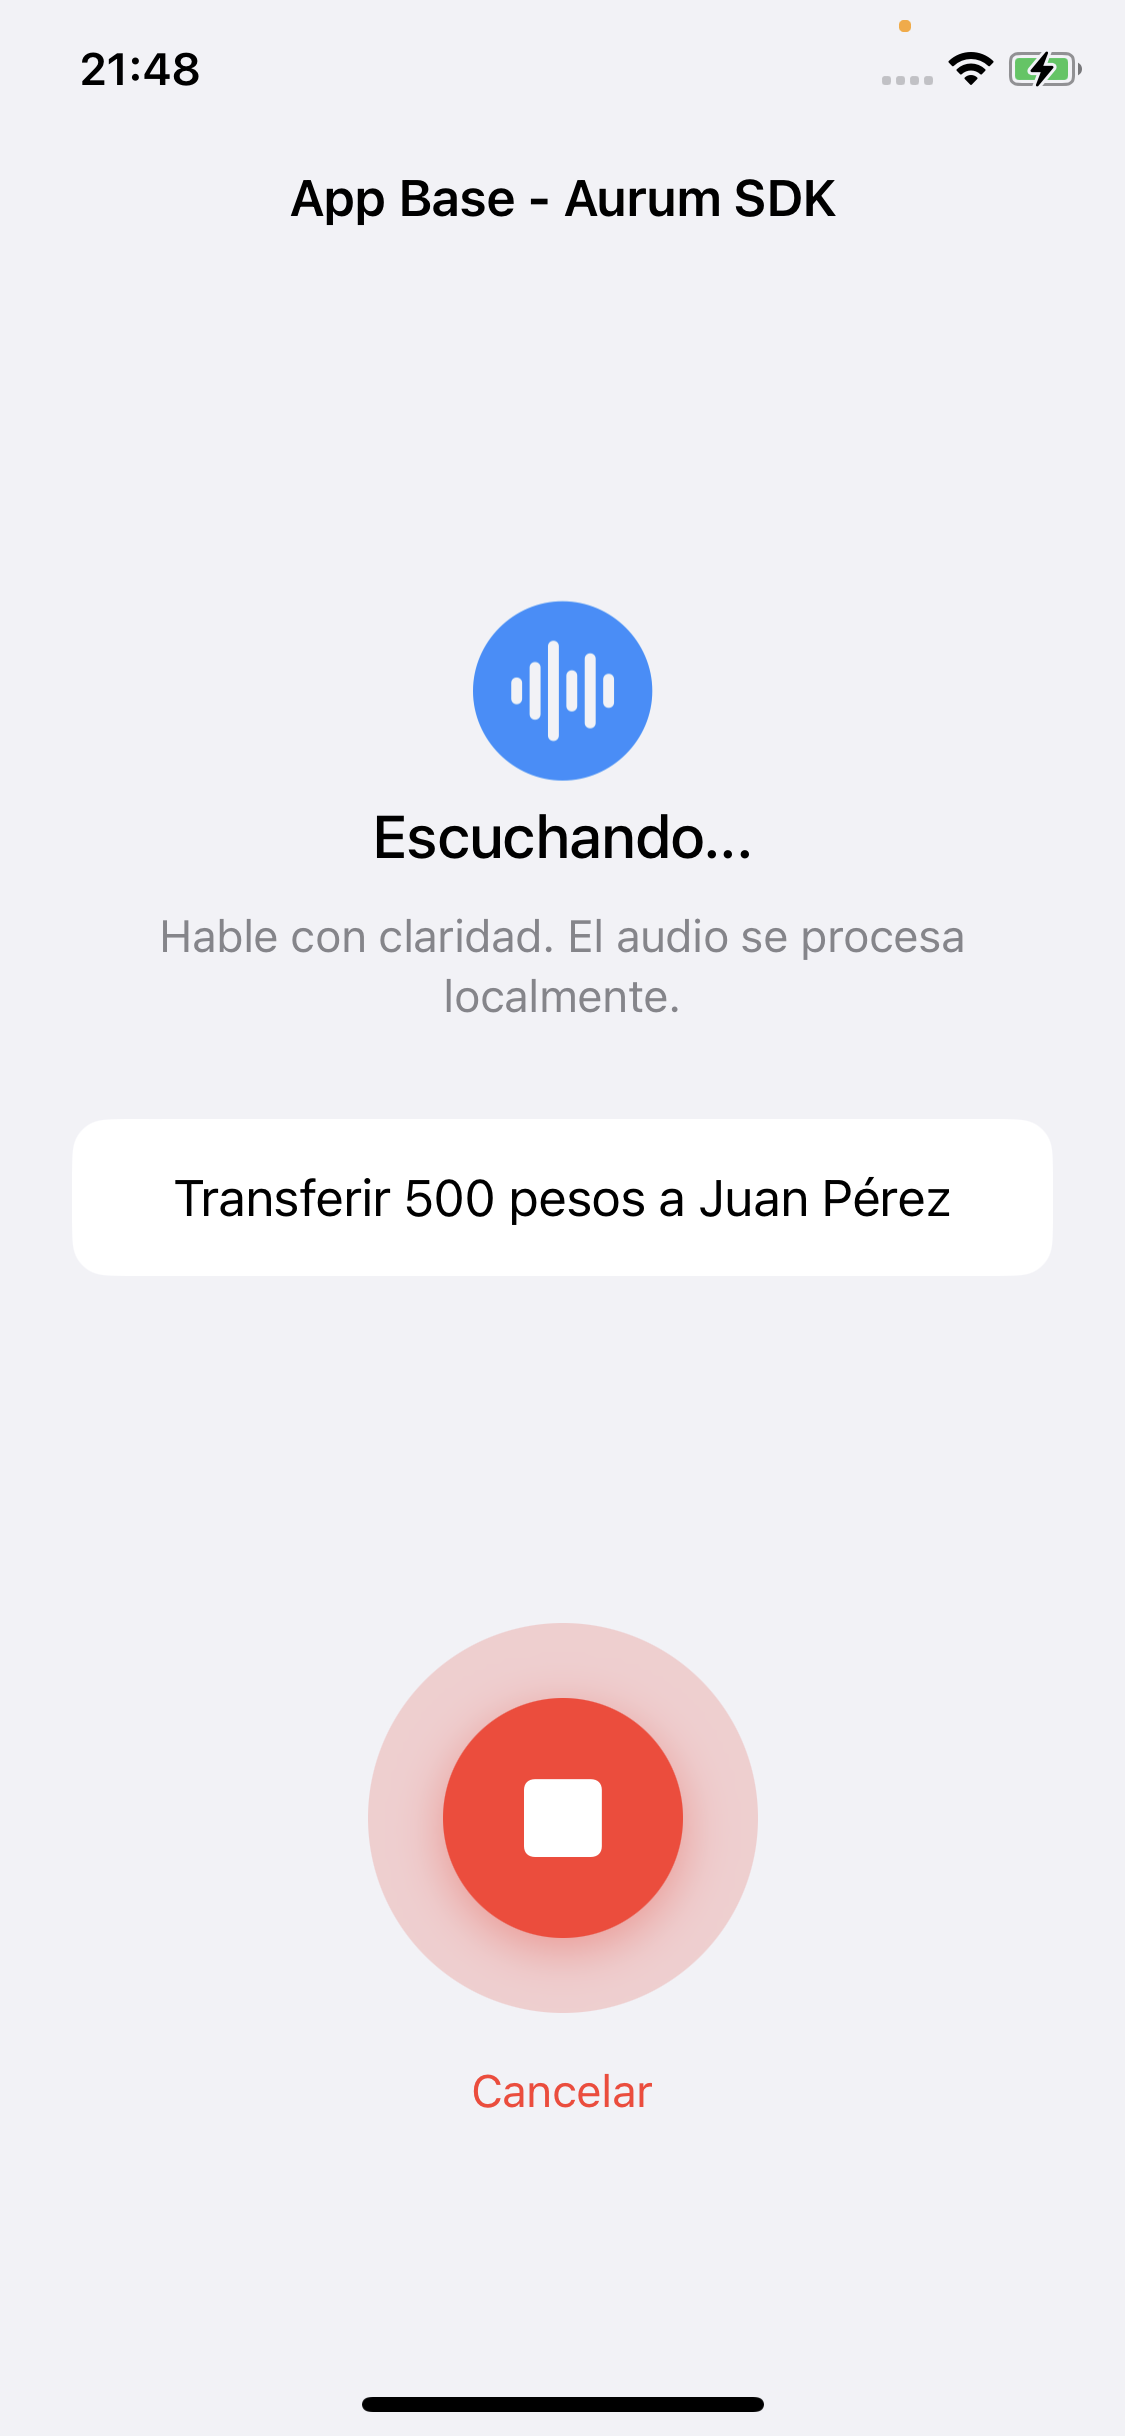
\includegraphics[width=0.85\textwidth]{./Figures/screenshots/transcripcion-dictado.PNG}
         \caption[Estado escuchando]{Estado \texttt{listening}: La transcripción parcial se muestra en tiempo real.}
         \label{fig:app-listening}
     \end{subfigure}
     \hfill
     \begin{subfigure}[b]{0.45\textwidth}
         \centering
         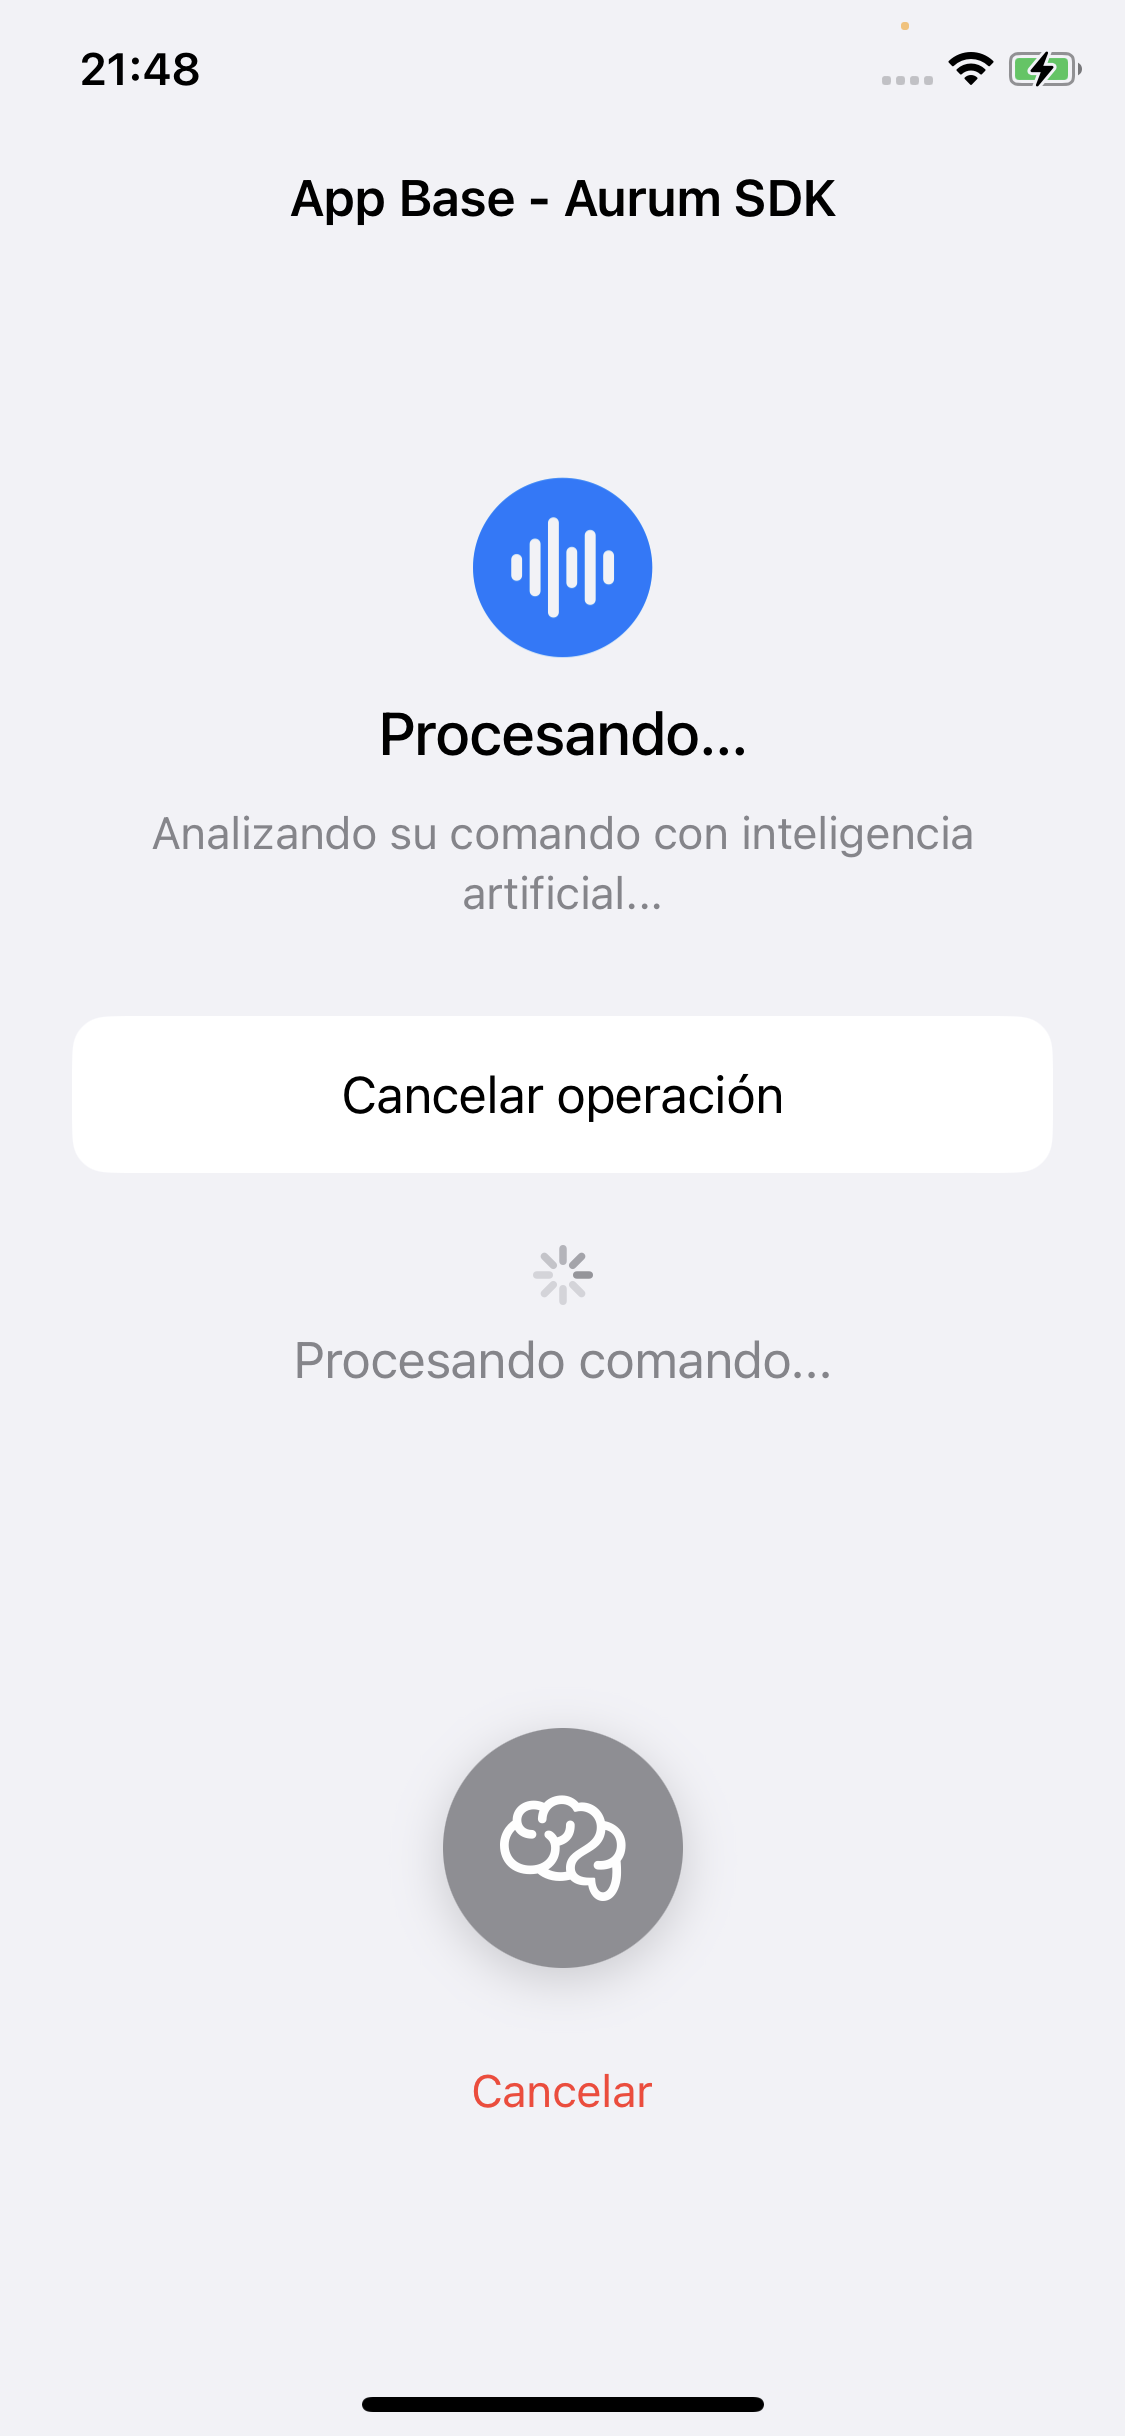
\includegraphics[width=0.85\textwidth]{./Figures/screenshots/procesamiento.PNG}
         \caption[Estado procesando audio a texto]{Estado \texttt{processing}: en este punto los modelos Core~ML ejecutan la inferencia.}
         \label{fig:app-processing}
     \end{subfigure}
        \caption{Capturas de pantalla que ilustran el funcionamiento de la transcripción en tiempo real y el procesamiento a texto.}
        \label{fig:working-state}
\end{figure}


\subsection{Resultados de usabilidad}
\label{subsec:resultados-usabilidad}

Los resultados de las pruebas de usabilidad arrojan las siguientes
observaciones:

\subsubsection*{Retroalimentación visual de la transcripción}

La visualización en tiempo real de la transcripción parcial en la \texttt{MainView} fue percibida como un elemento positivo de la experiencia.
La presencia de texto que se actualiza progresivamente mientras el usuario habla genera confianza en que el sistema está procesando activamente el comando, reduciendo la incertidumbre inherente a la interacción con sistemas de voz. En as tareas donde la transcripción mostró errores visibles (por ejemplo, en T2 cuando el reconocedor transcribió \texttt{luca} como \texttt{luca} sin convertirlo), los usuarios pudieron anticipar un posible error antes de ver la pantalla de confirmación.

\subsubsection*{Pantalla de confirmación}

El paso de confirmación obligatorio fue valorado positivamente en el contexto financiero. Los usuarios expresaron mayor confianza al poder verificar
visualmente el monto, la moneda y el destinatario antes de confirmar la operación. La presentación desglosada del \texttt{TransactionPayload}, especialmente el campo de \texttt{confianza} expresado como porcentaje, permitió a los usuarios evaluar la certeza del sistema y decidir de manera informada si confirmar o reintentar el comando.

La figura ~\ref{fig:confirm-transferencia} muestra la pantalla de confirmación de una transferencia detectada.

\begin{figure}[H]
	\centering
	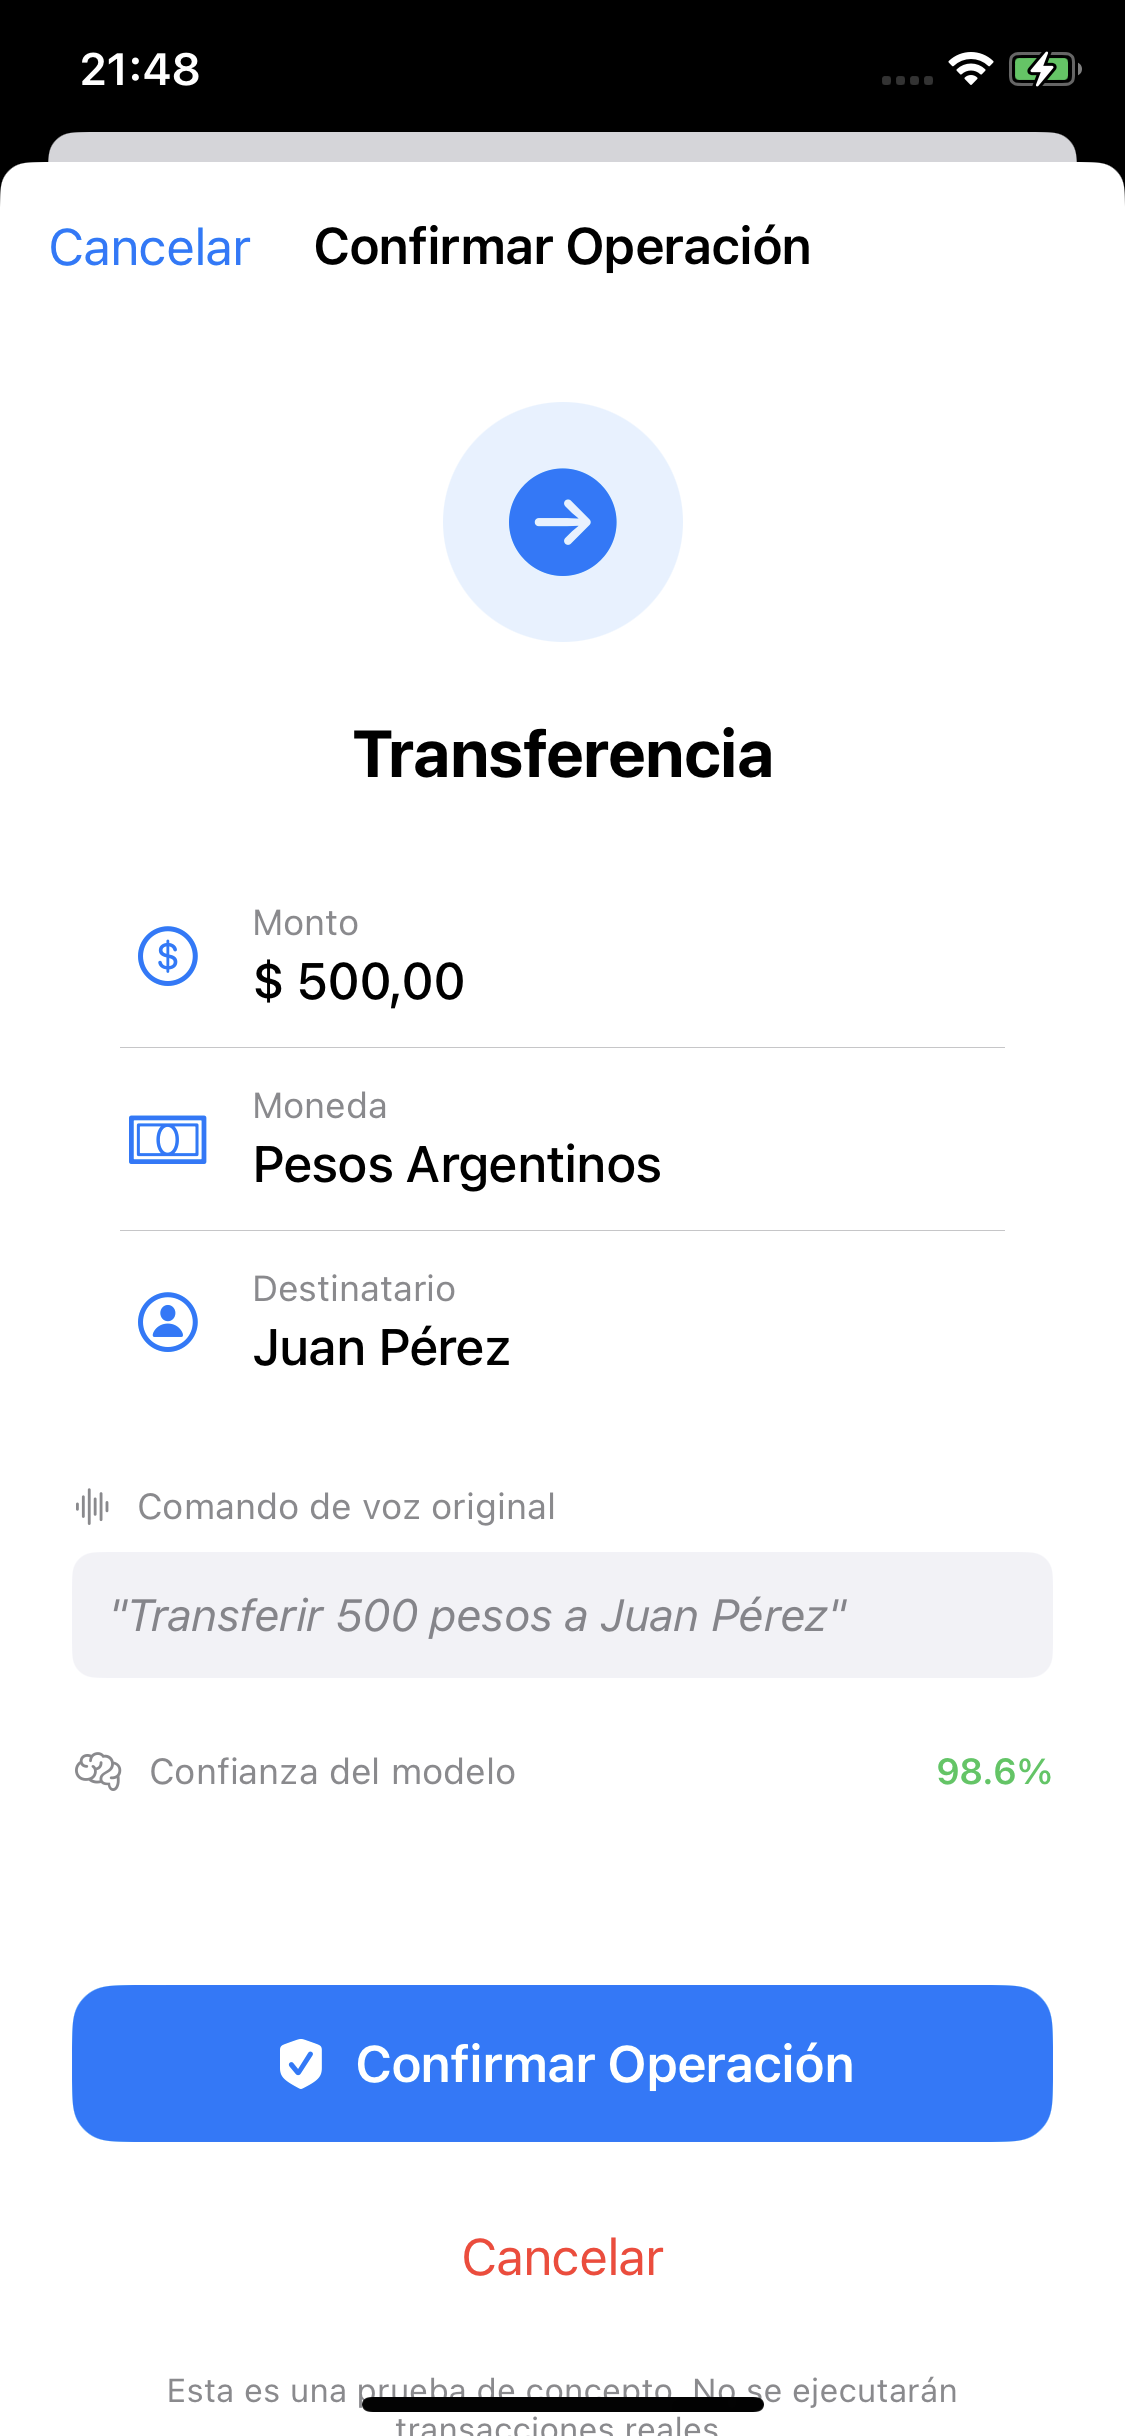
\includegraphics[width=0.35\textwidth]{./Figures/screenshots/intencion-confirmacion-transferencia.PNG}
	\caption[Pantalla de confirmación de transferencia]{Pantalla de confirmación para una transferencia exitosa. Se muestra el monto (\$~500,00), la moneda (Pesos Argentinos), el destinatario (Juan Pérez), la transcripción original y la confianza del modelo (98,6\%).}
	\label{fig:confirm-transferencia}
\end{figure}

La figura ~\ref{fig:confirm-saldo} muestra la pantalla de confirmación de una consulta de saldo.

\begin{figure}[H]
	\centering
	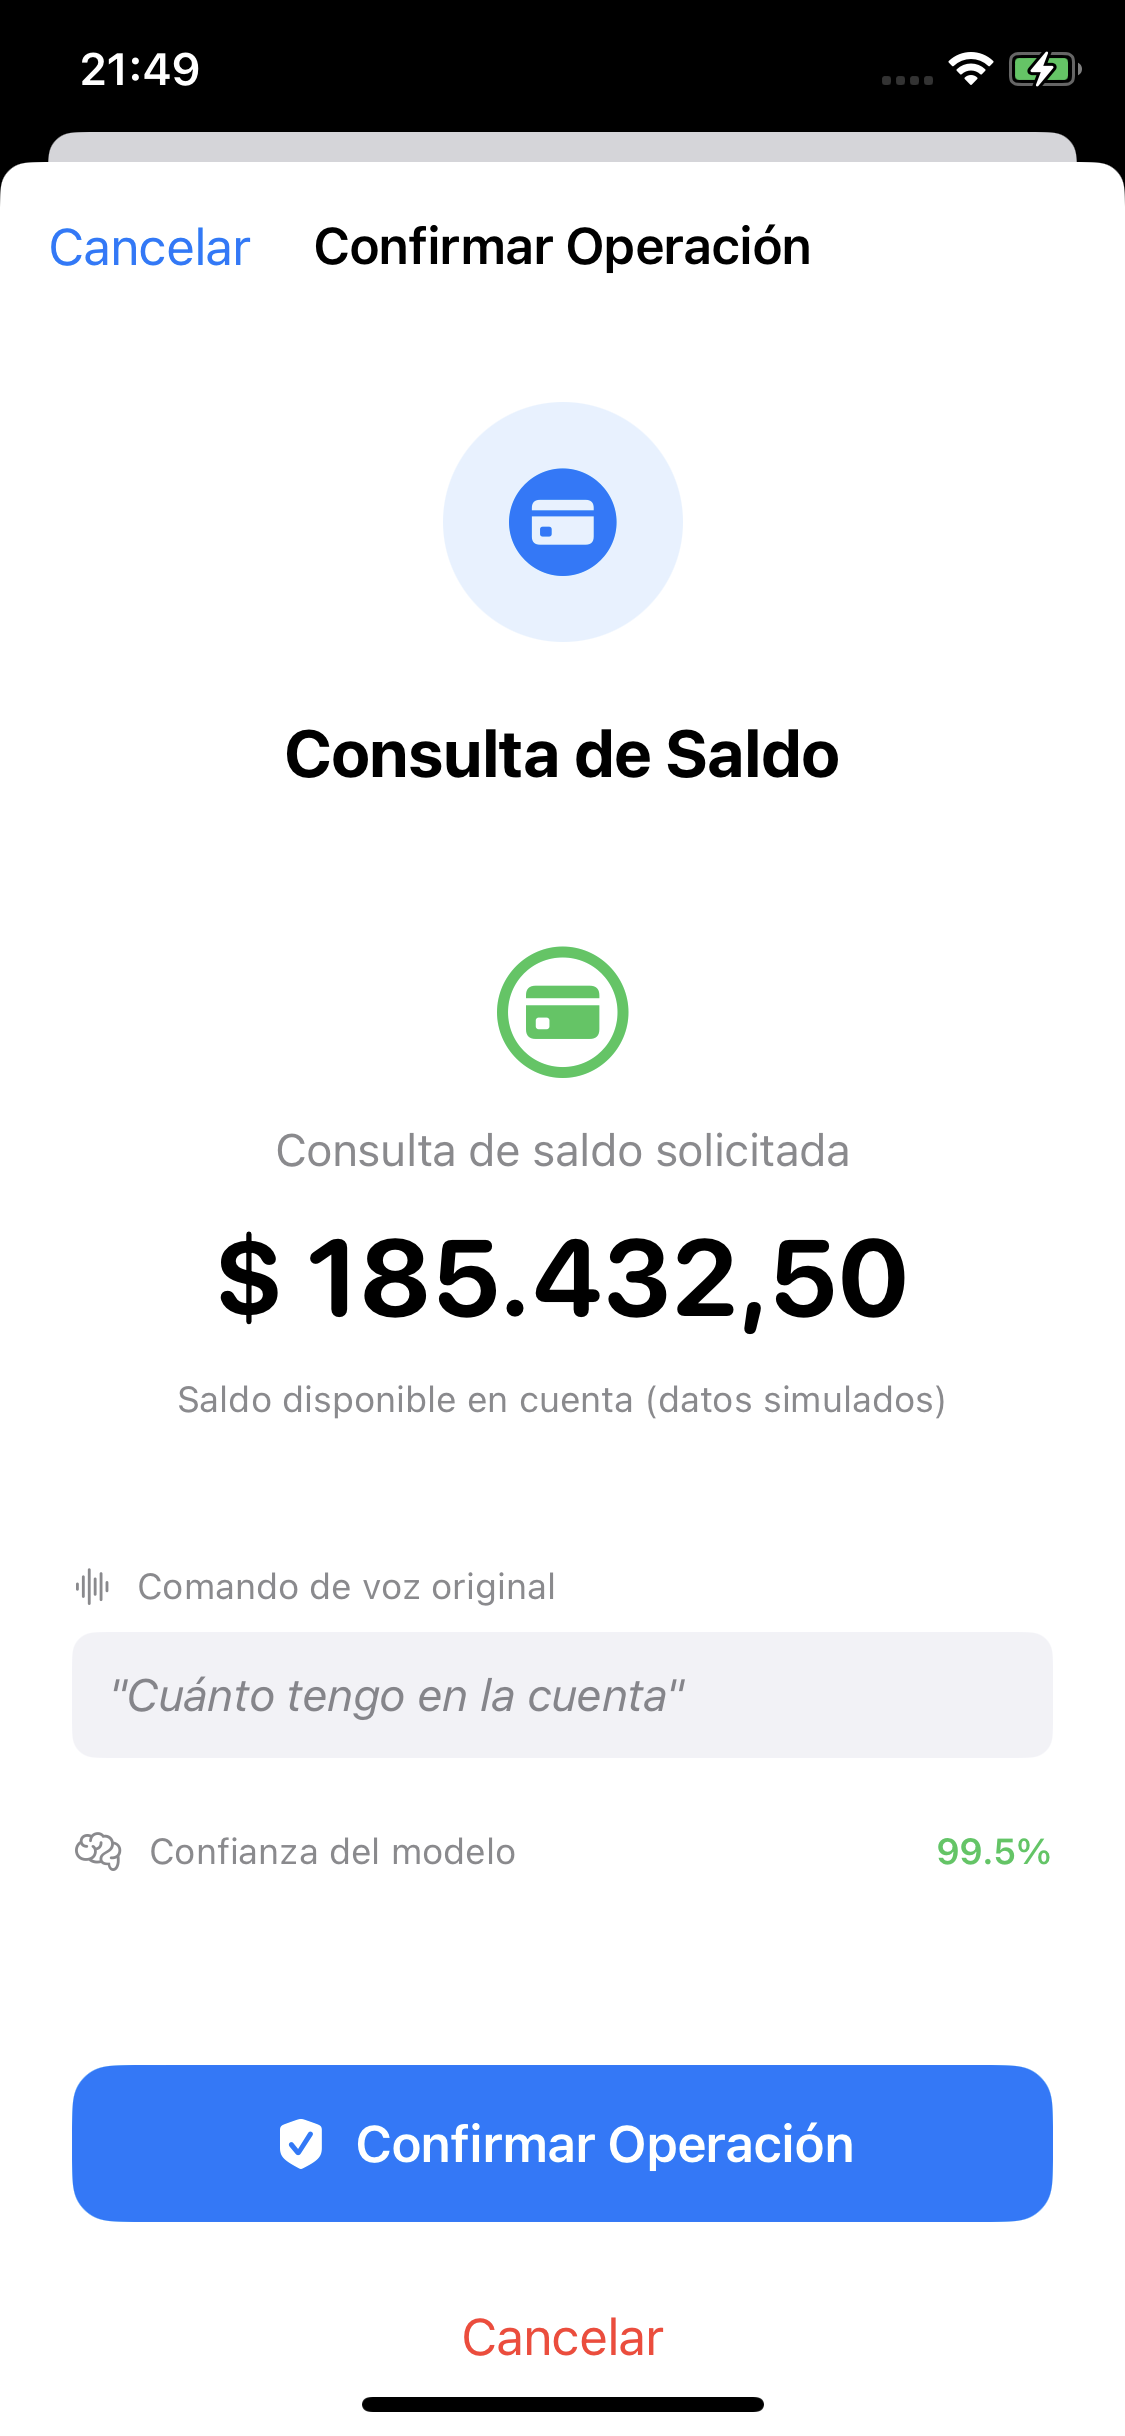
\includegraphics[width=0.45\textwidth]{./Figures/screenshots/intencion-consulta-saldo.PNG}
	\caption[Confirmación de consulta de saldo]{Confirmación de consulta de saldo. Se presenta el saldo simulado y la confianza del modelo (99,5\%).}
	\label{fig:confirm-saldo}
\end{figure}

La figura ~\ref{fig:confirm-cancelar} muestra la pantalla de confirmación de una anulación o cancelación de operación.

\begin{figure}[H]
	\centering
	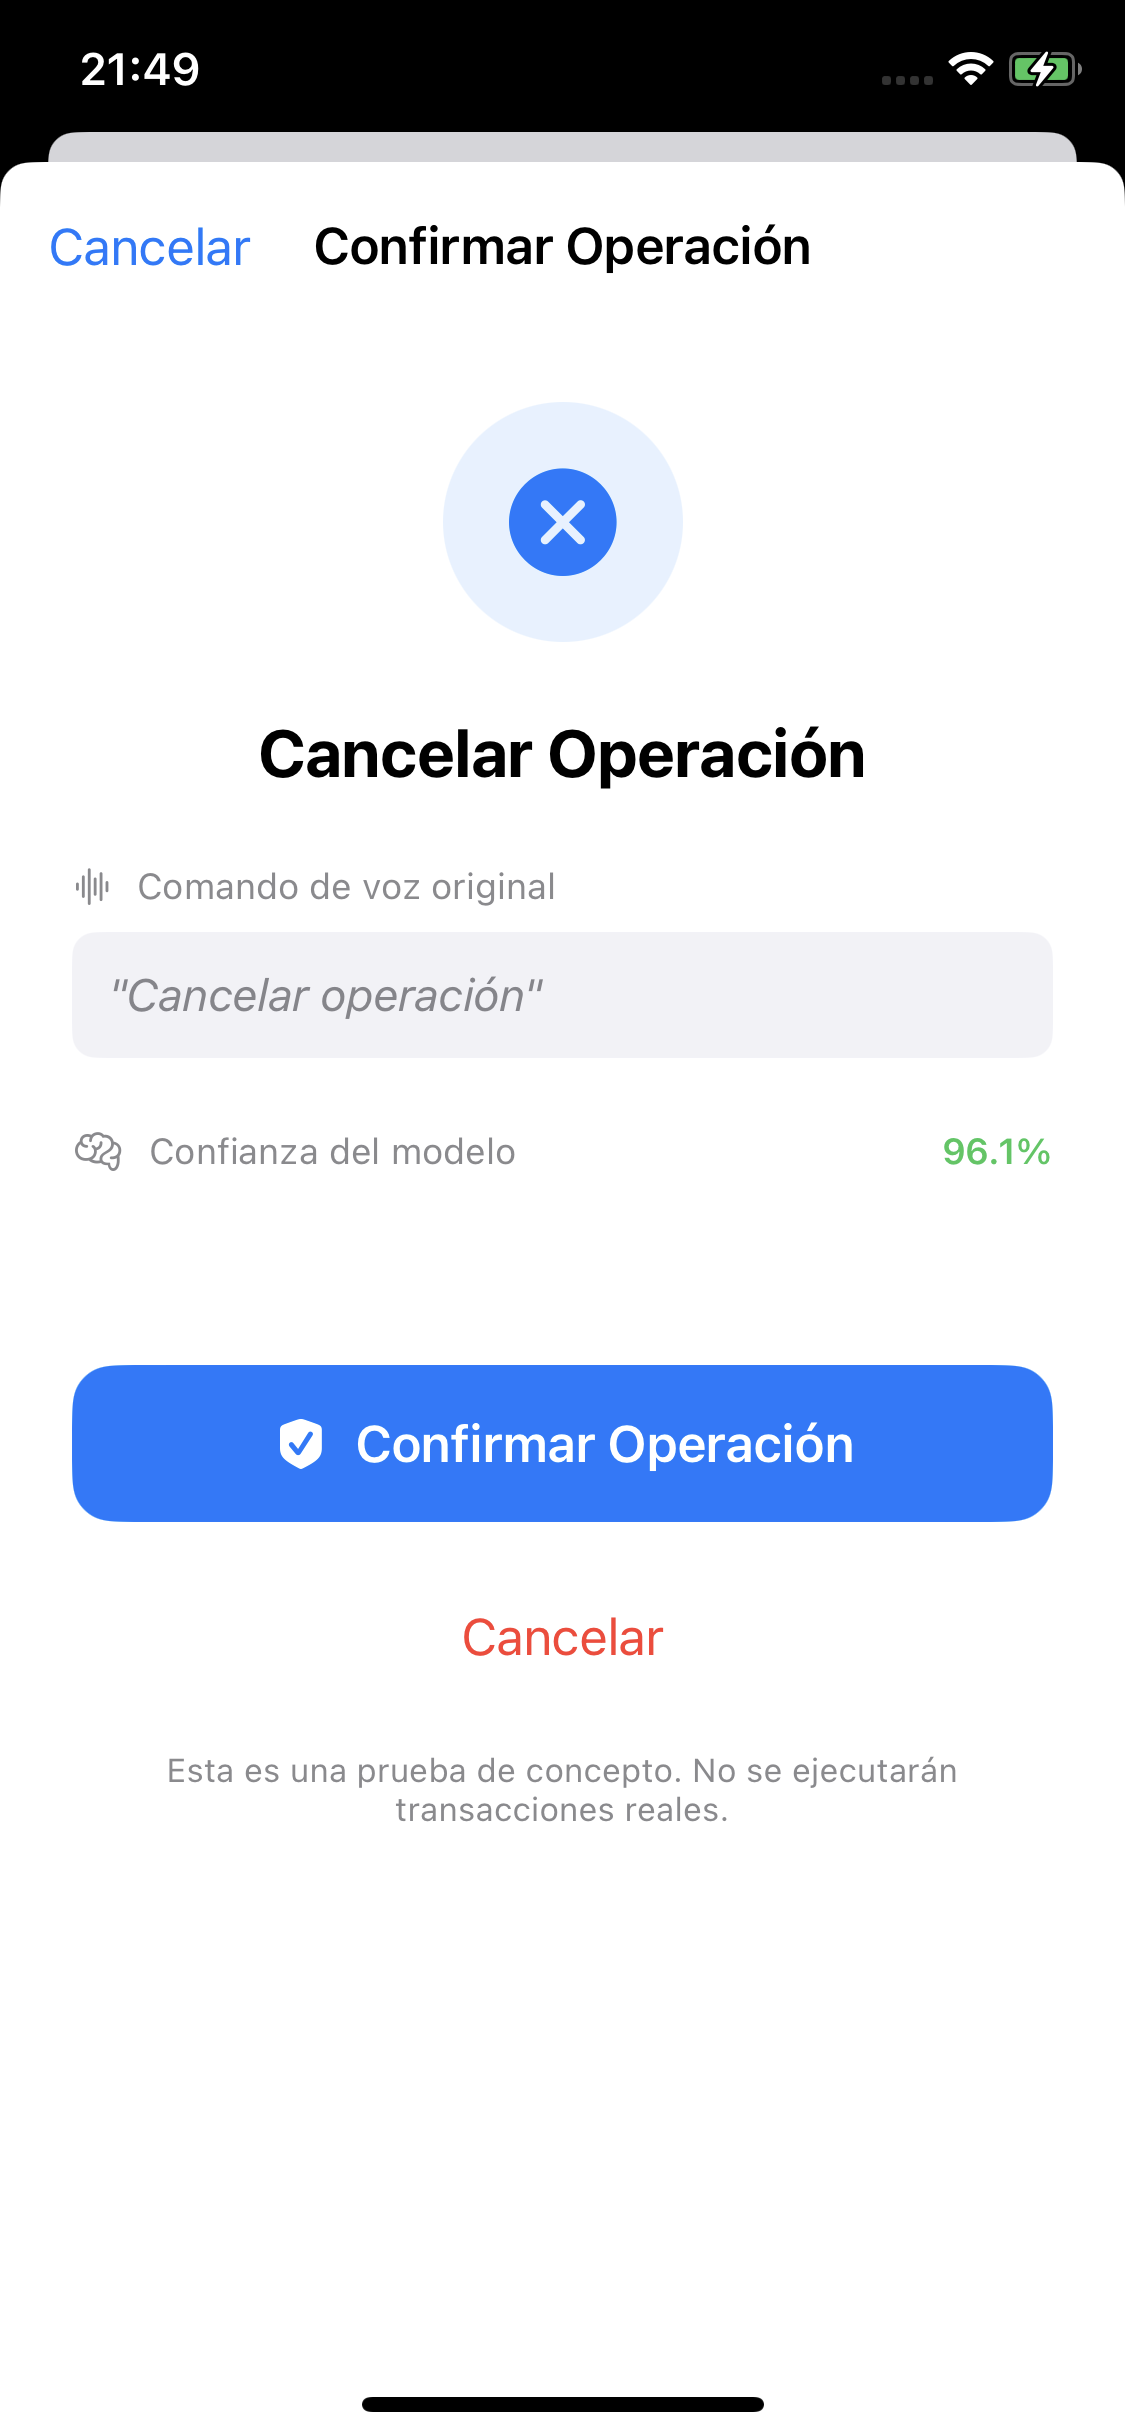
\includegraphics[width=0.45\textwidth]{./Figures/screenshots/intencion-cancelar.PNG}
	\caption[Confirmación de intención de cancelación]{Confirmación de intención de cancelación. El modelo clasificó el comando con una confianza de 96,1\%.}
	\label{fig:confirm-cancelar}
\end{figure}


\subsubsection*{Latencia percibida}

El tiempo transcurrido entre el fin del habla y la aparición de la pantalla de confirmación fue percibido como instantáneo en la mayoría de las tareas.
Esto es consistente con las mediciones de latencia reportadas en la sección~\ref{subsec:latencia}: el procesamiento NLU se completa en el orden de
los milisegundos, y la latencia dominante corresponde al \textit{Speech Framework}, que opera en modo \textit{streaming} y entrega la transcripción
final con un retardo del orden de 100--300~ms tras el último \textit{buffer} de audio.

\subsubsection*{Tarea ambigua (T6)}

La tarea T6 (\texttt{anular la transferencia de ayer}) fue incluida deliberadamente para evaluar el comportamiento del sistema ante un comando fuera del espacio de capacidades soportadas. La referencia temporal \texttt{de ayer} no es una entidad modelada, y la mezcla de \texttt{anular} con \texttt{transferencia} introduce ambigüedad entre las intenciones \textsc{cancelar} y \textsc{transferencia}. El comportamiento observado fue que el modelo clasificó el comando con una confianza inferior al umbral de 0,65, asignando la intención \texttt{.desconocida}. La aplicación base presentó un mensaje indicando que no pudo interpretar el comando, invitando al usuario a reformularlo. Este comportamiento es el deseado: el sistema prefiere rechazar un comando ambiguo
antes que ejecutar una operación financiera potencialmente incorrecta.

En la siguiente tabla ~\ref{tab:usabilidad} se ven reflejados los resultados de las pruebas realizadas:

% --- TABLA: Resultados de usabilidad ---
\begin{table}[H]
\caption{Resultados de las pruebas de usabilidad por tarea. La tasa de éxito
         se calcula sobre el total de intentos. El tiempo de interacción incluye
         el habla del usuario, el procesamiento y la confirmación.}

\centering
\label{tab:usabilidad}
\begin{tabular}{@{}lcccc@{}}
\toprule
\textbf{Tarea}
  & \textbf{Tasa de éxito}
  & \textbf{Tiempo medio}
  & \textbf{Errores}
  & \textbf{Intentos} \\
\midrule
T1 --- Transf. estándar   & 100\%  & 4,4 s & 0,0 & 1,0 \\
T2 --- Transf. coloquial  & 80\%   & 3,7 s & 0,6 & 1,8 \\
T3 --- Transf. dólares    & 100\%  & 3,9 s & 0,2 & 2,4 \\
T4 --- Consulta de saldo  & 100\%  & 3,3 s & 0,0 & 1,0 \\
T5 --- Cancelación        & 100\%  & 5,0 s & 0,0 & 3,2 \\
T6 --- Comando ambiguo    & 0\%    & 4,9 s & 3,4 & 3,4 \\
\midrule
\textit{Promedio}         & 80\%   & 4,2 s & 0,7 & --- \\
\bottomrule
\end{tabular}
\end{table}



% =============================================================================
% 4.4 ANÁLISIS DE RESULTADOS
% =============================================================================

\section{Análisis de resultados}
\label{sec:analisis}

Esta sección integra los resultados experimentales presentados en las secciones anteriores, los contrasta con el marco teórico establecido en el capítulo~2, y discute las implicancias para la viabilidad técnica de la solución propuesta.


\subsection{Validación de la hipótesis central}
\label{subsec:validacion-hipotesis}

La hipótesis central de este trabajo sostiene que es posible resolver, de forma íntegra en el dispositivo móvil, el problema dual de clasificar intenciones y extraer entidades nombradas a partir de comandos de voz financieros, utilizando exclusivamente los \textit{frameworks} nativos de Apple: Create~ML para el entrenamiento de modelos (MaxEnt para clasificación, CRF para etiquetado de secuencias) y los \textit{frameworks} \texttt{NaturalLanguage} y Core~ML para la inferencia local.

Los resultados obtenidos respaldan esta hipótesis. El clasificador de intenciones alcanzó un Macro F1-Score de 1,00 sobre el conjunto de test,
un valor que indica una capacidad discriminativa alta para las tres clases definidas. El extractor de entidades logró un Entity F1 \textit{strict} macro de 0,9369, que si bien es inferior al del clasificador, lo que es esperable dado que la extracción de entidades es intrínsecamente una tarea más compleja que la clasificación de texto, resulta suficiente para la prueba de concepto
propuesta.


\subsection{Comparación con arquitecturas alternativas}
\label{subsec:comparacion-arquitecturas}

La comparativa de arquitecturas presentada en el capítulo teórico estableció una comparación cualitativa entre tres familias de
arquitecturas: Transformers (BETO), redes recurrentes (BiLSTM) y frameworks nativos de Apple (Create~ML). Los resultados experimentales permiten ahora complementar esa comparación con evidencia cuantitativa.

En términos de precisión predictiva, la literatura reporta que modelos basados en BETO alcanzan F1-Scores del orden de 0,95--0,98 para clasificación de
intenciones en español \citep{canete2020spanish}, y que las arquitecturas BiLSTM-CRF obtienen valores de 0,88--0,93 para NER en dominios específicos \citep{lample2016neural}. Los valores obtenidos con Create~ML se ubican en un rango competitivo con los reportados para BiLSTM, aunque ligeramente inferiores a los de BETO.

Sin embargo, la comparación de precisión aislada es insuficiente. El análisis debe ponderarse con las restricciones operativas del \textit{edge computing}:

\begin{itemize}
    \item Tamaño del modelo: los modelos Create~ML ocupan menos de 1~MB en disco, frente a los $\sim$440~MB de BETO y los $\sim$5--15~MB de
    un BiLSTM. Para un dispositivo móvil con almacenamiento limitado y donde la aplicación bancaria compite por espacio con otras aplicaciones, esta
    diferencia de dos a tres órdenes de magnitud es determinante.

    \item Latencia de inferencia: los modelos nativos resolvieron el \textit{pipeline} completo en menos de 1~ms promedio. Un BETO sin comprimir
    requiere típicamente más de 200~ms por inferencia en un dispositivo móvil \citep{sun2020mobilebert}, lo que acumularía una latencia perceptible al
    ejecutar las dos inferencias (clasificación + NER) en secuencia.

    \item Integración nativa: los modelos Create~ML no requieren conversión con \texttt{coremltools} ni adaptaciones de formato. Se
    entrenan en macOS, se generan como \texttt{.mlmodel}, y Xcode los compila automáticamente a \texttt{.mlmodelc} al integrarlos al proyecto. Esta
    cadena de herramientas cerrada elimina una fuente significativa de errores de integración y mantenimiento.

    \item Privacidad nativa: al operar exclusivamente con frameworks de Apple, el sistema hereda las garantías de privacidad del ecosistema iOS.
    No se requiere configuración adicional para asegurar que los datos no abandonen el dispositivo, a diferencia de las arquitecturas basadas en
    PyTorch o TensorFlow que requieren validación explícita de que la inferencia se ejecuta localmente.
\end{itemize}

En síntesis, la pérdida marginal de precisión respecto a BETO se compensa con ventajas sustanciales en tamaño, latencia, facilidad de integración y
garantías de privacidad. Para el caso de uso específico de una prueba de concepto en el sector financiero argentino, donde la privacidad y la
latencia son requisitos no negociables, el \textit{trade-off} resulta favorable a la arquitectura nativa.


\subsection{Rol del \texttt{TextNormalizer}}
\label{subsec:rol-normalizer}

Los ensayos de robustez (tabla~\ref{tab:robustez}) evidencian el impacto crítico del componente \texttt{TextNormalizer} en el rendimiento del sistema.
Las categorías de coloquialismos y expresiones numéricas presentan una degradación moderada respecto a la línea base, lo que indica que el normalizador logra convertir una proporción significativa de las variaciones léxicas a formas canónicas que los modelos pueden interpretar.

No obstante, la categoría de mezcla de variaciones, donde confluyen coloquialismos, errores de STT y expresiones numéricas, exhibe la mayor
caída de rendimiento. Esto sugiere que el normalizador basado en reglas determinísticas (diccionarios de equivalencias y patrones de expresiones
regulares) alcanza un techo de capacidad cuando las variaciones se acumulan. Un enfoque más robusto podría complementar las reglas con un modelo de corrección ortográfica o un \textit{spell checker} adaptado al dominio financiero, capaz de recuperar tokens distorsionados por errores de
transcripción.


\subsection{Limitaciones del estudio}
\label{subsec:limitaciones}

Es pertinente explicitar las limitaciones del presente trabajo, tanto para contextualizar adecuadamente los resultados como para orientar el trabajo
futuro:

\begin{enumerate}
    \item Corpus sintético: los modelos fueron entrenados y evaluados sobre un corpus generado mediante plantillas y aumentación de datos. Si
    bien esta estrategia permite controlar la distribución de clases y entidades, no captura la totalidad de la variabilidad lingüística del habla
    espontánea. Un corpus recolectado a partir de grabaciones de usuarios reales proporcionaría una evaluación más representativa.

    \item Dominio acotado: el sistema soporta únicamente tres intenciones y tres tipos de entidades. Una aplicación bancaria productiva
    requeriría un catálogo significativamente más amplio de operaciones (pagos de servicios, inversiones, consultas de movimientos, etc.) y entidades
    (fechas, números de cuenta, CBU/CVU).

    \item Idioma único: la implementación se centra exclusivamente en español rioplatense. Si bien el reconocedor de voz utiliza un mecanismo de \textit{fallback} que selecciona automáticamente el locale con soporte \textit{on-device} (\texttt{es-MX} o \texttt{es-ES}), los modelos NLU y el normalizador fueron entrenados y configurados para el léxico rioplatense. La generalización a otros dialectos del español o a otros idiomas requeriría corpus de entrenamiento adicionales y la validación de que el \texttt{Text\allowbreak{}Normalizer} es extensible a otros sistemas léxicos coloquiales.

    \item Ausencia de \textit{backend} real: la aplicación base simula la confirmación de la transacción sin conectarse a un sistema bancario real.
    La integración con una API transaccional introduciría latencias de red, requisitos de autenticación biométrica (Face~ID, Touch~ID) y manejo de
    errores de conectividad que están fuera del alcance de esta prueba de concepto.

    \item Mediciones de latencia en macOS: el benchmark de latencia se ejecutó sobre la CPU del equipo de desarrollo (macOS), no sobre un
    dispositivo iOS físico. Si bien los valores obtenidos ya se encuentran por debajo del umbral de percepción, una medición en dispositivo con Xcode
    Instruments proporcionaría datos más representativos del rendimiento en producción.

    \item Pruebas de usabilidad limitadas: el protocolo de usabilidad se diseñó como evaluación exploratoria con un número reducido de
    participantes. Un estudio de usabilidad riguroso requeriría una muestra más amplia, diversificada en edad, familiaridad con tecnología de voz y
    dialecto regional.
\end{enumerate}


\subsection{Conexión con CRISP-DM}
\label{subsec:crisp-dm}

El desarrollo de este trabajo siguió la metodología CRISP-DM (\textit{Cross Industry Standard Process for Data Mining}) como marco organizativo del ciclo de vida del proyecto de \textit{machine learning}. Los resultados obtenidos en esta fase de evaluación retroalimentan el ciclo y permiten identificar las intervenciones prioritarias para una eventual iteración:

\begin{itemize}
    \item Comprensión de los datos: los errores de la entidad \textsc{destinatario} señalan la necesidad de enriquecer el corpus con
    mayor variabilidad de nombres propios, incluyendo apodos, sobrenombres y nombres compuestos más largos.

    \item Preparación de los datos: la degradación ante errores de STT sugiere incorporar \textit{noise injection} al proceso de aumentación:
    generar variantes con errores tipográficos y fonéticos simulados para que los modelos desarrollen tolerancia a tokens ruidosos.

    \item Modelado: si las iteraciones de datos no alcanzan los umbrales deseados, podría evaluarse la migración del clasificador de
    MaxEnt a \textit{Transfer Learning} con \texttt{.dynamicEmbedding}, que aprovecha embeddings contextuales preentrenados por Apple a costa de
    un incremento moderado en el tamaño del modelo y el tiempo de entrenamiento.

    \item Despliegue: la validación positiva de la latencia y la privacidad \textit{on-device} confirma la viabilidad técnica del
    despliegue en dispositivos iOS reales, estableciendo la base para una fase piloto con usuarios del sector financiero.
\end{itemize}

\medskip

La tabla~\ref{tab:resumen-resultados} condensa los indicadores clave de
rendimiento de los modelos Core~ML del SDK Aurum.

% --- TABLA 7: Resumen ejecutivo ---
\begin{table}[H]
\caption{Resumen de rendimiento de los modelos Core ML del SDK Aurum.}
\centering
\begin{tabular}{@{}lcc@{}}
\toprule
\textbf{Métrica} & \textbf{Clasificador} & \textbf{Extractor NER} \\
                  & \textbf{(MaxEnt)}     & \textbf{(CRF)} \\
\midrule
Accuracy / Token Accuracy     & 100,00\% & 89,65\% \\
Macro F1-Score                & 1,0000   & 0,9491   \\
Entity F1 (strict)            & ---     & 0,9369   \\
Entity F1 (relaxed)           & ---     & 0,9369   \\
Tamaño del modelo             & 3,1 KB   & 407,2 KB   \\
Latencia media de inferencia  & 0,02 ms  & 0,26 ms  \\
\bottomrule
\end{tabular}
\label{tab:resumen-resultados}
\end{table}

% Chapter 5: Conclusiones

\chapter{Conclusiones} % Main chapter title

\label{Chapter5}

En este capítulo se presentan las conclusiones generales derivadas del desarrollo de la prueba de concepto y se proponen líneas de trabajo futuro que permitirían evolucionar el prototipo hacia un producto integrable en un entorno bancario productivo.


%----------------------------------------------------------------------------------------
%	SECTION 1
%----------------------------------------------------------------------------------------

\section{Resultados generales}

El presente trabajo demostró la viabilidad técnica de implementar un sistema de transacciones financieras por voz que opera de forma completamente local en dispositivos móviles iOS. A continuación se enumeran los principales logros alcanzados:

\begin{itemize}
\item Se diseñó e implementó el SDK Aurum como \textit{framework} nativo reutilizable, que encapsula la totalidad del \textit{pipeline} de procesamiento de voz: captura de audio, transcripción, normalización e inferencia de modelos de \textit{machine learning}. Su arquitectura basada en el patrón de delegación permite que cualquier aplicación bancaria lo integre implementando un único protocolo público.

\item Se entrenaron dos modelos de \textit{machine learning} con Create~ML (MaxEnt para clasificación de intenciones y CRF para extracción de entidades) que alcanzaron un desempeño satisfactorio para la prueba de concepto: 100\% de \textit{accuracy} en la clasificación de intenciones y un F1 \textit{strict} de 0,9369 en la extracción de entidades, con tamaños de modelo de 3,1~KB y 407,2~KB respectivamente.

\item Se validó que el procesamiento estrictamente local (\textit{on-device}) es factible en el hardware actual de Apple. Los modelos Core~ML resolvieron el \textit{pipeline} completo de inferencia con latencias del orden de fracciones de milisegundo, muy por debajo del umbral de percepción humana de 100~ms establecido por Nielsen.

\item Se garantizó la privacidad por diseño: en ningún momento del flujo los datos de audio ni las transcripciones abandonan el dispositivo físico, lo que satisface las restricciones de confidencialidad exigidas por el sector financiero y se alinea con la Ley argentina de Protección de Datos Personales (Ley 25.326).

\item Se desarrolló una aplicación base funcional con SwiftUI que valida la integración con el SDK y demuestra el flujo completo de interacción: desde la activación del micrófono hasta la presentación del \textit{payload} estructurado en una pantalla de confirmación.

\item La metodología CRISP-DM resultó adecuada para estructurar las fases del proyecto, lo que permitió iterar entre la comprensión del dominio financiero, la generación del \textit{dataset} sintético, el entrenamiento de los modelos y la evaluación de resultados.
\end{itemize}

En cuanto a las dificultades encontradas, la principal fue la ausencia de datos reales de comandos de voz bancarios, resuelta mediante la generación de un corpus sintético con técnicas de aumentación de datos. Adicionalmente, se identificó que el locale \texttt{es-AR} no dispone de modelo de reconocimiento de voz \textit{on-device} en la mayoría de los dispositivos iOS, lo que requirió implementar un mecanismo de selección automática de locale con \textit{fallback} a \texttt{es-MX}.

En síntesis, los resultados obtenidos validan que la convergencia entre los \textit{frameworks} nativos de Apple (Speech, Core~ML, Natural\-Language) y las técnicas de procesamiento de lenguaje natural permite construir soluciones de voz robustas, privadas y de baja latencia para el dominio financiero, sin dependencia de servicios en la nube.


%----------------------------------------------------------------------------------------
%	SECTION 2
%----------------------------------------------------------------------------------------

\section{Próximos pasos}

El presente trabajo establece las bases técnicas para una solución de voz bancaria \textit{on-device}. A continuación se proponen las líneas de trabajo futuro que permitirían acercar el prototipo a un nivel de madurez productivo:

\begin{itemize}
\item Validación con usuarios reales: ejecutar un estudio de usabilidad con una muestra amplia y diversificada en edad, dialecto regional y familiaridad con tecnología de voz, que permita obtener métricas estadísticamente significativas de tasa de éxito, tiempo de interacción y satisfacción.

\item Ampliación del corpus de entrenamiento: incorporar grabaciones de voz reales (con consentimiento informado) para entrenar los modelos con datos representativos del habla natural, incluyendo ruido ambiental, variaciones prosódicas y errores de dicción.

\item Expansión del dominio transaccional: extender las intenciones soportadas a operaciones como pagos de servicios, consultas de últimos movimientos, inversiones y operaciones con tarjetas, lo que implicaría ampliar el esquema de entidades y reentrenar los modelos.

\item Mediciones en dispositivo físico: ejecutar \textit{benchmarks} de latencia con Xcode Instruments sobre dispositivos iPhone con Neural Engine, lo que proporcionaría datos de rendimiento representativos del entorno de producción.

\item Integración con biometría de voz: investigar la factibilidad de incorporar un módulo de verificación de identidad basado en las características acústicas del hablante (\textit{speaker verification}), que operaría como factor adicional de autenticación previo a la ejecución de la transacción.

\item Soporte multilingüe: adaptar el \textit{pipeline} para soportar otros idiomas y variantes regionales del español, aprovechando la arquitectura modular del SDK que permite intercambiar modelos sin modificar la lógica de orquestación.

\item Evaluación de seguridad adversarial: analizar la robustez del sistema ante ataques de inyección acústica (\textit{adversarial audio attacks}) y definir contramedidas, como umbrales adaptativos de confianza y detección de anomalías en la señal de entrada.

\item Integración con el \textit{core} bancario: diseñar la capa de comunicación segura entre el SDK y los servicios \textit{backend} del banco, incluyendo la firma criptográfica del \textit{payload}, la autenticación mutua TLS y la trazabilidad de las operaciones para auditoría.
\end{itemize}


%----------------------------------------------------------------------------------------
% Apéndices
%----------------------------------------------------------------------------------------

\appendix

% Incluir apéndices desde archivos separados si es necesario
%\include{Appendices/AppendixA}

%----------------------------------------------------------------------------------------
% Bibliografía
%----------------------------------------------------------------------------------------

\renewcommand{\bibname}{Bibliografía} % Para asegurarte de que el título sea correcto
\phantomsection % Necesario para que el enlace del marcador sea correcto

\printbibliography[heading=bibintoc]

\end{document}






